\documentclass[aspectratio=169,11pt]{beamer}

\newcommand{\currentpart}{4}
% ============================================================================
% Quantitative Research -- shared preamble for all five slide decks
%
% Every deck starts with
%     \documentclass[aspectratio=169,11pt]{beamer}
%     % ============================================================================
% Quantitative Research -- shared preamble for all five slide decks
%
% Every deck starts with
%     \documentclass[aspectratio=169,11pt]{beamer}
%     % ============================================================================
% Quantitative Research -- shared preamble for all five slide decks
%
% Every deck starts with
%     \documentclass[aspectratio=169,11pt]{beamer}
%     \input{../common/preamble.tex}
%     \newcommand{\currentpart}{<k>}
% so that layout, colours, boxes and code listings are identical everywhere.
% ============================================================================

% ======================== Packages ========================
\usepackage[utf8]{inputenc}
\usepackage[T1]{fontenc}
\usepackage[english]{babel}
\usepackage{graphicx}
\usepackage{booktabs}
\usepackage{amsmath,amssymb,amsfonts}
\usepackage{mathtools}
\usepackage{xcolor}
\usepackage{colortbl}
\usepackage{array}
\usepackage{multicol}
\usepackage{verbatim}          % provides the comment environment
\usepackage{tikz}
\usepackage{pgfplots}
\pgfplotsset{compat=1.18}
\usetikzlibrary{arrows.meta,positioning,fit,backgrounds,shapes.geometric,calc,decorations.pathreplacing}
\usepackage{listings}
\usepackage{hyperref}
\usepackage{pgfpages}          % notes on a second screen (only if enabled)

% ======================== Speaker notes (talk-tracks) ========================
% The decks compile WITHOUT notes by default. To get a version with the
% talk-tracks, uncomment exactly ONE of the lines below and recompile:
% \setbeameroption{show notes}                          % notes as separate pages
% \setbeameroption{show notes on second screen=right}   % slides left, notes right

% ======================== Math fonts ========================
% Beamer typesets text in sans serif; make \mathrm and \mathbf match it
% (otherwise SE, TP, RSS print in serif and \mathbf falls back to non-bold).
\renewcommand{\bfdefault}{bx}   % CM sans has bold extended (bx) only
\DeclareMathAlphabet{\mathrm}{T1}{cmss}{m}{n}
\DeclareMathAlphabet{\mathbf}{T1}{cmss}{bx}{n}
\SetMathAlphabet{\mathrm}{bold}{T1}{cmss}{bx}{n}
\SetMathAlphabet{\mathbf}{bold}{T1}{cmss}{bx}{n}
\SetSymbolFont{operators}{bold}{OT1}{cmss}{bx}{n}
% Beamer re-declares \mathrm at \begin{document}; re-apply the sans-serif version
\AtBeginDocument{\SetMathAlphabet{\mathrm}{normal}{T1}{cmss}{m}{n}%
                 \SetMathAlphabet{\mathrm}{bold}{T1}{cmss}{bx}{n}}

% ======================== Colour palette (matched to plots / Madrid) ========
\definecolor{hsbiblau}{HTML}{3333B2}
\definecolor{hsbiblaudunkel}{HTML}{1C1C6E}
\definecolor{hsbiorange}{HTML}{E69F00}
\definecolor{hsbigrau}{HTML}{9A9A9A}
\definecolor{hsbirot}{HTML}{C0392B}
\definecolor{hsbigruen}{HTML}{2E8B57}
\definecolor{hsbiviolett}{HTML}{8C3CA0}   % 4th comparison colour (e.g. candidate lines)

% ======================== Theme ========================
\usetheme{Madrid}
\usecolortheme{default}
\setbeamertemplate{navigation symbols}{}
\setbeamertemplate{blocks}[rounded][shadow=false]
\setbeamerfont{section in head/foot}{size=\tiny}

% Horizontal section navigation bar in the headline
\setbeamertemplate{headline}{%
  \leavevmode%
  \hbox{%
    \begin{beamercolorbox}[wd=\paperwidth,ht=2.5ex,dp=1.125ex]{section in head/foot}%
      \scriptsize\insertsectionnavigationhorizontal{\paperwidth}{}{\hskip0pt plus1filll}%
    \end{beamercolorbox}%
  }%
}

% Footline: lecture part, current section (if any) and slide number
\newcommand{\footsection}{%
  \setbox0=\hbox{\insertsection}%
  \ifdim\wd0>0pt\ \textbar\ \insertsection\fi}
\setbeamertemplate{footline}{%
  \leavevmode%
  \hbox{%
  \begin{beamercolorbox}[wd=\paperwidth,ht=2.5ex,dp=1.125ex]{author in head/foot}%
    \hspace*{2em}Part~\currentpart\footsection\hfill\insertframenumber{}/\inserttotalframenumber\hspace*{2em}%
  \end{beamercolorbox}%
  }%
}

% Automatic section overview slide. Decks with many sections define
%   \newcommand{\overviewleft}{1-4}\newcommand{\overviewright}{5-8}
% before \begin{document} to get a two-column overview.
\newcommand{\overviewtoc}[1]{%
  \tableofcontents[currentsection,sectionstyle=show/shaded,
                   subsectionstyle=show/show/hide,sections={#1}]}
\newcommand{\sectionoverview}{%
  \ifdefined\overviewleft
    \begin{columns}[T]
      \column{0.49\textwidth}\overviewtoc{\overviewleft}
      \column{0.49\textwidth}\overviewtoc{\overviewright}
    \end{columns}%
  \else
    \tableofcontents[currentsection,sectionstyle=show/shaded,
                     subsectionstyle=show/show/hide]%
  \fi}
\AtBeginSection[]{%
  \begin{frame}{Overview}
    \scriptsize
    \sectionoverview
  \end{frame}%
}

% ======================== Python listing style ========================
\lstdefinestyle{Pystyle}{
  language=Python,
  basicstyle=\ttfamily\footnotesize,
  keywordstyle=\color{hsbiblau},
  commentstyle=\color{hsbigrau}\itshape,
  stringstyle=\color{teal},
  showstringspaces=false,
  literate={~}{{$\sim$}}1
           {–}{{--}}1 {—}{{---}}1 {ä}{{\"a}}1 {ö}{{\"o}}1 {ü}{{\"u}}1
           {Ä}{{\"A}}1 {Ö}{{\"O}}1 {Ü}{{\"U}}1 {ß}{{\ss}}1 {é}{{\'e}}1,
  upquote=true,
  columns=fixed, basewidth=0.5em
}
% Plain style for printed Python output (fixed columns keep tables aligned)
\lstdefinestyle{Pyout}{
  language={},
  basicstyle=\ttfamily\scriptsize,
  keywordstyle={}, commentstyle={}, stringstyle={},
  columns=fixed, keepspaces=true, basewidth=0.52em,
  showstringspaces=false,
  upquote=true,
  literate={~}{{$\sim$}}1 {–}{{--}}1 {—}{{---}}1 {‘}{{`}}1 {’}{{'}}1,
}
\lstset{style=Pystyle}

% ======================== Custom commands / styles ========================
\newcommand{\kernaussage}[1]{\begin{alertblock}{Key takeaway}#1\end{alertblock}}
\newcommand{\inworten}[1]{{\small\textbf{\textcolor{hsbiblaudunkel}{In words:}}~#1}}
\newcommand{\guidingquestion}[1]{\begin{exampleblock}{Guiding question}#1\end{exampleblock}}
\newcommand{\appendixnote}[1]{\par\vfill\vspace{-1.6ex}\hfill{\scriptsize\itshape\textcolor{hsbiblau}{$\rightarrow$ Appendix: #1}}\par\vspace{-1ex}}
\newcommand{\sourcenote}[1]{\vfill\hfill{\tiny\itshape\color{gray}Source: #1}\par}

% Companion notebooks (Jupyter / Google Colab). Every deck defines
%     \newcommand{\notebookpath}{Part_k_<Topic>/Part_k_<Topic>.ipynb}
% \trynotebook{<notebook section>} prints a small clickable pointer at the
% bottom right of a frame that opens the deck's notebook in Google Colab
% (the same notebook lies next to the .tex file for local Jupyter use).
\newcommand{\colaburl}{https://colab.research.google.com/github/ChrisW09/Quantitative-Research-Methods/blob/main/}
\newcommand{\trynotebook}[1]{\par\vfill\vspace{-1.6ex}\hfill{\scriptsize\href{\colaburl\notebookpath}{\textcolor{hsbiorange!85!black}{$\blacktriangleright$\ \textbf{Try it yourself:} notebook, #1 \ -- open in Colab}}}\par\vspace{-1ex}}

% Reusable TikZ styles for concept diagrams
\tikzset{
  flowbox/.style={rounded corners, draw=hsbiblaudunkel, very thick,
                  fill=hsbiblau!10, align=center, inner sep=5pt, minimum height=8mm},
  flowboxo/.style={rounded corners, draw=hsbiorange!85!black, very thick,
                   fill=hsbiorange!18, align=center, inner sep=5pt, minimum height=8mm},
  flowboxg/.style={rounded corners, draw=hsbigrau!90!black, very thick,
                   fill=hsbigrau!15, align=center, inner sep=5pt, minimum height=8mm},
  flowarr/.style={-{Latex[length=2.6mm,width=2mm]}, line width=1pt, draw=hsbiblaudunkel},
}

% ======================== Course overview (same slide in every deck) ========
% \courseoverview highlights the part given by \currentpart.
\newcommand{\cpart}[2]{%
  \ifnum\currentpart=#1\relax
    \textcolor{hsbiblau}{\textbf{#2}}%
  \else
    #2%
  \fi}
\newcommand{\courseoverview}{%
\begin{frame}{The lecture at a glance}
  \begin{center}
    \small\renewcommand{\arraystretch}{1.15}
    \begin{tabular}{@{}l l >{\raggedright\arraybackslash}p{9.2cm}@{}}
      \toprule
      & \textbf{Part} & \textbf{Content} \\
      \midrule
      \ifnum\currentpart=1 $\blacktriangleright$\fi & \cpart{1}{1 -- Descriptive Statistics}
        & \cpart{1}{Basic concepts, levels of measurement, frequencies, measures of central tendency and dispersion} \\
      \ifnum\currentpart=2 $\blacktriangleright$\fi & \cpart{2}{2 -- Graphical Representations}
        & \cpart{2}{Empirical CDF, histogram, boxplot} \\
      \ifnum\currentpart=3 $\blacktriangleright$\fi & \cpart{3}{3 -- Statistical Inference}
        & \cpart{3}{Normal distribution and CLT, confidence intervals, sample size, hypothesis tests, $p$-values, one-sided tests, types of error} \\
      \ifnum\currentpart=4 $\blacktriangleright$\fi & \cpart{4}{4 -- Regression}
        & \cpart{4}{Correlation, least squares, goodness of fit, inference for regression, multiple regression (appendix: residual analysis)} \\
      \ifnum\currentpart=5 $\blacktriangleright$\fi & \cpart{5}{5 -- Classification}
        & \cpart{5}{Conditional probability, logistic regression, classification rules, confusion matrix, base rates, ROC/AUC, Bayes classifiers} \\
      \bottomrule
    \end{tabular}
  \end{center}
  \begin{center}
    \footnotesize All analyses are carried out in \textbf{Python} (NumPy,
    pandas, SciPy, statsmodels, matplotlib); every deck comes with a Python
    script that reproduces its numbers and a Jupyter notebook with all
    examples and exercises -- also in Google Colab.
  \end{center}
\end{frame}}

% ======================== Title information (shared) ========================
\title{Quantitative Research}
\author{Prof.\ Dr.\ Christoph Weisser}
\institute{}
\date{}   % must stay explicitly empty -- otherwise Beamer prints today's date

\graphicspath{{images/}}

%     \newcommand{\currentpart}{<k>}
% so that layout, colours, boxes and code listings are identical everywhere.
% ============================================================================

% ======================== Packages ========================
\usepackage[utf8]{inputenc}
\usepackage[T1]{fontenc}
\usepackage[english]{babel}
\usepackage{graphicx}
\usepackage{booktabs}
\usepackage{amsmath,amssymb,amsfonts}
\usepackage{mathtools}
\usepackage{xcolor}
\usepackage{colortbl}
\usepackage{array}
\usepackage{multicol}
\usepackage{verbatim}          % provides the comment environment
\usepackage{tikz}
\usepackage{pgfplots}
\pgfplotsset{compat=1.18}
\usetikzlibrary{arrows.meta,positioning,fit,backgrounds,shapes.geometric,calc,decorations.pathreplacing}
\usepackage{listings}
\usepackage{hyperref}
\usepackage{pgfpages}          % notes on a second screen (only if enabled)

% ======================== Speaker notes (talk-tracks) ========================
% The decks compile WITHOUT notes by default. To get a version with the
% talk-tracks, uncomment exactly ONE of the lines below and recompile:
% \setbeameroption{show notes}                          % notes as separate pages
% \setbeameroption{show notes on second screen=right}   % slides left, notes right

% ======================== Math fonts ========================
% Beamer typesets text in sans serif; make \mathrm and \mathbf match it
% (otherwise SE, TP, RSS print in serif and \mathbf falls back to non-bold).
\renewcommand{\bfdefault}{bx}   % CM sans has bold extended (bx) only
\DeclareMathAlphabet{\mathrm}{T1}{cmss}{m}{n}
\DeclareMathAlphabet{\mathbf}{T1}{cmss}{bx}{n}
\SetMathAlphabet{\mathrm}{bold}{T1}{cmss}{bx}{n}
\SetMathAlphabet{\mathbf}{bold}{T1}{cmss}{bx}{n}
\SetSymbolFont{operators}{bold}{OT1}{cmss}{bx}{n}
% Beamer re-declares \mathrm at \begin{document}; re-apply the sans-serif version
\AtBeginDocument{\SetMathAlphabet{\mathrm}{normal}{T1}{cmss}{m}{n}%
                 \SetMathAlphabet{\mathrm}{bold}{T1}{cmss}{bx}{n}}

% ======================== Colour palette (matched to plots / Madrid) ========
\definecolor{hsbiblau}{HTML}{3333B2}
\definecolor{hsbiblaudunkel}{HTML}{1C1C6E}
\definecolor{hsbiorange}{HTML}{E69F00}
\definecolor{hsbigrau}{HTML}{9A9A9A}
\definecolor{hsbirot}{HTML}{C0392B}
\definecolor{hsbigruen}{HTML}{2E8B57}
\definecolor{hsbiviolett}{HTML}{8C3CA0}   % 4th comparison colour (e.g. candidate lines)

% ======================== Theme ========================
\usetheme{Madrid}
\usecolortheme{default}
\setbeamertemplate{navigation symbols}{}
\setbeamertemplate{blocks}[rounded][shadow=false]
\setbeamerfont{section in head/foot}{size=\tiny}

% Horizontal section navigation bar in the headline
\setbeamertemplate{headline}{%
  \leavevmode%
  \hbox{%
    \begin{beamercolorbox}[wd=\paperwidth,ht=2.5ex,dp=1.125ex]{section in head/foot}%
      \scriptsize\insertsectionnavigationhorizontal{\paperwidth}{}{\hskip0pt plus1filll}%
    \end{beamercolorbox}%
  }%
}

% Footline: lecture part, current section (if any) and slide number
\newcommand{\footsection}{%
  \setbox0=\hbox{\insertsection}%
  \ifdim\wd0>0pt\ \textbar\ \insertsection\fi}
\setbeamertemplate{footline}{%
  \leavevmode%
  \hbox{%
  \begin{beamercolorbox}[wd=\paperwidth,ht=2.5ex,dp=1.125ex]{author in head/foot}%
    \hspace*{2em}Part~\currentpart\footsection\hfill\insertframenumber{}/\inserttotalframenumber\hspace*{2em}%
  \end{beamercolorbox}%
  }%
}

% Automatic section overview slide. Decks with many sections define
%   \newcommand{\overviewleft}{1-4}\newcommand{\overviewright}{5-8}
% before \begin{document} to get a two-column overview.
\newcommand{\overviewtoc}[1]{%
  \tableofcontents[currentsection,sectionstyle=show/shaded,
                   subsectionstyle=show/show/hide,sections={#1}]}
\newcommand{\sectionoverview}{%
  \ifdefined\overviewleft
    \begin{columns}[T]
      \column{0.49\textwidth}\overviewtoc{\overviewleft}
      \column{0.49\textwidth}\overviewtoc{\overviewright}
    \end{columns}%
  \else
    \tableofcontents[currentsection,sectionstyle=show/shaded,
                     subsectionstyle=show/show/hide]%
  \fi}
\AtBeginSection[]{%
  \begin{frame}{Overview}
    \scriptsize
    \sectionoverview
  \end{frame}%
}

% ======================== Python listing style ========================
\lstdefinestyle{Pystyle}{
  language=Python,
  basicstyle=\ttfamily\footnotesize,
  keywordstyle=\color{hsbiblau},
  commentstyle=\color{hsbigrau}\itshape,
  stringstyle=\color{teal},
  showstringspaces=false,
  literate={~}{{$\sim$}}1
           {–}{{--}}1 {—}{{---}}1 {ä}{{\"a}}1 {ö}{{\"o}}1 {ü}{{\"u}}1
           {Ä}{{\"A}}1 {Ö}{{\"O}}1 {Ü}{{\"U}}1 {ß}{{\ss}}1 {é}{{\'e}}1,
  upquote=true,
  columns=fixed, basewidth=0.5em
}
% Plain style for printed Python output (fixed columns keep tables aligned)
\lstdefinestyle{Pyout}{
  language={},
  basicstyle=\ttfamily\scriptsize,
  keywordstyle={}, commentstyle={}, stringstyle={},
  columns=fixed, keepspaces=true, basewidth=0.52em,
  showstringspaces=false,
  upquote=true,
  literate={~}{{$\sim$}}1 {–}{{--}}1 {—}{{---}}1 {‘}{{`}}1 {’}{{'}}1,
}
\lstset{style=Pystyle}

% ======================== Custom commands / styles ========================
\newcommand{\kernaussage}[1]{\begin{alertblock}{Key takeaway}#1\end{alertblock}}
\newcommand{\inworten}[1]{{\small\textbf{\textcolor{hsbiblaudunkel}{In words:}}~#1}}
\newcommand{\guidingquestion}[1]{\begin{exampleblock}{Guiding question}#1\end{exampleblock}}
\newcommand{\appendixnote}[1]{\par\vfill\vspace{-1.6ex}\hfill{\scriptsize\itshape\textcolor{hsbiblau}{$\rightarrow$ Appendix: #1}}\par\vspace{-1ex}}
\newcommand{\sourcenote}[1]{\vfill\hfill{\tiny\itshape\color{gray}Source: #1}\par}

% Companion notebooks (Jupyter / Google Colab). Every deck defines
%     \newcommand{\notebookpath}{Part_k_<Topic>/Part_k_<Topic>.ipynb}
% \trynotebook{<notebook section>} prints a small clickable pointer at the
% bottom right of a frame that opens the deck's notebook in Google Colab
% (the same notebook lies next to the .tex file for local Jupyter use).
\newcommand{\colaburl}{https://colab.research.google.com/github/ChrisW09/Quantitative-Research-Methods/blob/main/}
\newcommand{\trynotebook}[1]{\par\vfill\vspace{-1.6ex}\hfill{\scriptsize\href{\colaburl\notebookpath}{\textcolor{hsbiorange!85!black}{$\blacktriangleright$\ \textbf{Try it yourself:} notebook, #1 \ -- open in Colab}}}\par\vspace{-1ex}}

% Reusable TikZ styles for concept diagrams
\tikzset{
  flowbox/.style={rounded corners, draw=hsbiblaudunkel, very thick,
                  fill=hsbiblau!10, align=center, inner sep=5pt, minimum height=8mm},
  flowboxo/.style={rounded corners, draw=hsbiorange!85!black, very thick,
                   fill=hsbiorange!18, align=center, inner sep=5pt, minimum height=8mm},
  flowboxg/.style={rounded corners, draw=hsbigrau!90!black, very thick,
                   fill=hsbigrau!15, align=center, inner sep=5pt, minimum height=8mm},
  flowarr/.style={-{Latex[length=2.6mm,width=2mm]}, line width=1pt, draw=hsbiblaudunkel},
}

% ======================== Course overview (same slide in every deck) ========
% \courseoverview highlights the part given by \currentpart.
\newcommand{\cpart}[2]{%
  \ifnum\currentpart=#1\relax
    \textcolor{hsbiblau}{\textbf{#2}}%
  \else
    #2%
  \fi}
\newcommand{\courseoverview}{%
\begin{frame}{The lecture at a glance}
  \begin{center}
    \small\renewcommand{\arraystretch}{1.15}
    \begin{tabular}{@{}l l >{\raggedright\arraybackslash}p{9.2cm}@{}}
      \toprule
      & \textbf{Part} & \textbf{Content} \\
      \midrule
      \ifnum\currentpart=1 $\blacktriangleright$\fi & \cpart{1}{1 -- Descriptive Statistics}
        & \cpart{1}{Basic concepts, levels of measurement, frequencies, measures of central tendency and dispersion} \\
      \ifnum\currentpart=2 $\blacktriangleright$\fi & \cpart{2}{2 -- Graphical Representations}
        & \cpart{2}{Empirical CDF, histogram, boxplot} \\
      \ifnum\currentpart=3 $\blacktriangleright$\fi & \cpart{3}{3 -- Statistical Inference}
        & \cpart{3}{Normal distribution and CLT, confidence intervals, sample size, hypothesis tests, $p$-values, one-sided tests, types of error} \\
      \ifnum\currentpart=4 $\blacktriangleright$\fi & \cpart{4}{4 -- Regression}
        & \cpart{4}{Correlation, least squares, goodness of fit, inference for regression, multiple regression (appendix: residual analysis)} \\
      \ifnum\currentpart=5 $\blacktriangleright$\fi & \cpart{5}{5 -- Classification}
        & \cpart{5}{Conditional probability, logistic regression, classification rules, confusion matrix, base rates, ROC/AUC, Bayes classifiers} \\
      \bottomrule
    \end{tabular}
  \end{center}
  \begin{center}
    \footnotesize All analyses are carried out in \textbf{Python} (NumPy,
    pandas, SciPy, statsmodels, matplotlib); every deck comes with a Python
    script that reproduces its numbers and a Jupyter notebook with all
    examples and exercises -- also in Google Colab.
  \end{center}
\end{frame}}

% ======================== Title information (shared) ========================
\title{Quantitative Research}
\author{Prof.\ Dr.\ Christoph Weisser}
\institute{}
\date{}   % must stay explicitly empty -- otherwise Beamer prints today's date

\graphicspath{{images/}}

%     \newcommand{\currentpart}{<k>}
% so that layout, colours, boxes and code listings are identical everywhere.
% ============================================================================

% ======================== Packages ========================
\usepackage[utf8]{inputenc}
\usepackage[T1]{fontenc}
\usepackage[english]{babel}
\usepackage{graphicx}
\usepackage{booktabs}
\usepackage{amsmath,amssymb,amsfonts}
\usepackage{mathtools}
\usepackage{xcolor}
\usepackage{colortbl}
\usepackage{array}
\usepackage{multicol}
\usepackage{verbatim}          % provides the comment environment
\usepackage{tikz}
\usepackage{pgfplots}
\pgfplotsset{compat=1.18}
\usetikzlibrary{arrows.meta,positioning,fit,backgrounds,shapes.geometric,calc,decorations.pathreplacing}
\usepackage{listings}
\usepackage{hyperref}
\usepackage{pgfpages}          % notes on a second screen (only if enabled)

% ======================== Speaker notes (talk-tracks) ========================
% The decks compile WITHOUT notes by default. To get a version with the
% talk-tracks, uncomment exactly ONE of the lines below and recompile:
% \setbeameroption{show notes}                          % notes as separate pages
% \setbeameroption{show notes on second screen=right}   % slides left, notes right

% ======================== Math fonts ========================
% Beamer typesets text in sans serif; make \mathrm and \mathbf match it
% (otherwise SE, TP, RSS print in serif and \mathbf falls back to non-bold).
\renewcommand{\bfdefault}{bx}   % CM sans has bold extended (bx) only
\DeclareMathAlphabet{\mathrm}{T1}{cmss}{m}{n}
\DeclareMathAlphabet{\mathbf}{T1}{cmss}{bx}{n}
\SetMathAlphabet{\mathrm}{bold}{T1}{cmss}{bx}{n}
\SetMathAlphabet{\mathbf}{bold}{T1}{cmss}{bx}{n}
\SetSymbolFont{operators}{bold}{OT1}{cmss}{bx}{n}
% Beamer re-declares \mathrm at \begin{document}; re-apply the sans-serif version
\AtBeginDocument{\SetMathAlphabet{\mathrm}{normal}{T1}{cmss}{m}{n}%
                 \SetMathAlphabet{\mathrm}{bold}{T1}{cmss}{bx}{n}}

% ======================== Colour palette (matched to plots / Madrid) ========
\definecolor{hsbiblau}{HTML}{3333B2}
\definecolor{hsbiblaudunkel}{HTML}{1C1C6E}
\definecolor{hsbiorange}{HTML}{E69F00}
\definecolor{hsbigrau}{HTML}{9A9A9A}
\definecolor{hsbirot}{HTML}{C0392B}
\definecolor{hsbigruen}{HTML}{2E8B57}
\definecolor{hsbiviolett}{HTML}{8C3CA0}   % 4th comparison colour (e.g. candidate lines)

% ======================== Theme ========================
\usetheme{Madrid}
\usecolortheme{default}
\setbeamertemplate{navigation symbols}{}
\setbeamertemplate{blocks}[rounded][shadow=false]
\setbeamerfont{section in head/foot}{size=\tiny}

% Horizontal section navigation bar in the headline
\setbeamertemplate{headline}{%
  \leavevmode%
  \hbox{%
    \begin{beamercolorbox}[wd=\paperwidth,ht=2.5ex,dp=1.125ex]{section in head/foot}%
      \scriptsize\insertsectionnavigationhorizontal{\paperwidth}{}{\hskip0pt plus1filll}%
    \end{beamercolorbox}%
  }%
}

% Footline: lecture part, current section (if any) and slide number
\newcommand{\footsection}{%
  \setbox0=\hbox{\insertsection}%
  \ifdim\wd0>0pt\ \textbar\ \insertsection\fi}
\setbeamertemplate{footline}{%
  \leavevmode%
  \hbox{%
  \begin{beamercolorbox}[wd=\paperwidth,ht=2.5ex,dp=1.125ex]{author in head/foot}%
    \hspace*{2em}Part~\currentpart\footsection\hfill\insertframenumber{}/\inserttotalframenumber\hspace*{2em}%
  \end{beamercolorbox}%
  }%
}

% Automatic section overview slide. Decks with many sections define
%   \newcommand{\overviewleft}{1-4}\newcommand{\overviewright}{5-8}
% before \begin{document} to get a two-column overview.
\newcommand{\overviewtoc}[1]{%
  \tableofcontents[currentsection,sectionstyle=show/shaded,
                   subsectionstyle=show/show/hide,sections={#1}]}
\newcommand{\sectionoverview}{%
  \ifdefined\overviewleft
    \begin{columns}[T]
      \column{0.49\textwidth}\overviewtoc{\overviewleft}
      \column{0.49\textwidth}\overviewtoc{\overviewright}
    \end{columns}%
  \else
    \tableofcontents[currentsection,sectionstyle=show/shaded,
                     subsectionstyle=show/show/hide]%
  \fi}
\AtBeginSection[]{%
  \begin{frame}{Overview}
    \scriptsize
    \sectionoverview
  \end{frame}%
}

% ======================== Python listing style ========================
\lstdefinestyle{Pystyle}{
  language=Python,
  basicstyle=\ttfamily\footnotesize,
  keywordstyle=\color{hsbiblau},
  commentstyle=\color{hsbigrau}\itshape,
  stringstyle=\color{teal},
  showstringspaces=false,
  literate={~}{{$\sim$}}1
           {–}{{--}}1 {—}{{---}}1 {ä}{{\"a}}1 {ö}{{\"o}}1 {ü}{{\"u}}1
           {Ä}{{\"A}}1 {Ö}{{\"O}}1 {Ü}{{\"U}}1 {ß}{{\ss}}1 {é}{{\'e}}1,
  upquote=true,
  columns=fixed, basewidth=0.5em
}
% Plain style for printed Python output (fixed columns keep tables aligned)
\lstdefinestyle{Pyout}{
  language={},
  basicstyle=\ttfamily\scriptsize,
  keywordstyle={}, commentstyle={}, stringstyle={},
  columns=fixed, keepspaces=true, basewidth=0.52em,
  showstringspaces=false,
  upquote=true,
  literate={~}{{$\sim$}}1 {–}{{--}}1 {—}{{---}}1 {‘}{{`}}1 {’}{{'}}1,
}
\lstset{style=Pystyle}

% ======================== Custom commands / styles ========================
\newcommand{\kernaussage}[1]{\begin{alertblock}{Key takeaway}#1\end{alertblock}}
\newcommand{\inworten}[1]{{\small\textbf{\textcolor{hsbiblaudunkel}{In words:}}~#1}}
\newcommand{\guidingquestion}[1]{\begin{exampleblock}{Guiding question}#1\end{exampleblock}}
\newcommand{\appendixnote}[1]{\par\vfill\vspace{-1.6ex}\hfill{\scriptsize\itshape\textcolor{hsbiblau}{$\rightarrow$ Appendix: #1}}\par\vspace{-1ex}}
\newcommand{\sourcenote}[1]{\vfill\hfill{\tiny\itshape\color{gray}Source: #1}\par}

% Companion notebooks (Jupyter / Google Colab). Every deck defines
%     \newcommand{\notebookpath}{Part_k_<Topic>/Part_k_<Topic>.ipynb}
% \trynotebook{<notebook section>} prints a small clickable pointer at the
% bottom right of a frame that opens the deck's notebook in Google Colab
% (the same notebook lies next to the .tex file for local Jupyter use).
\newcommand{\colaburl}{https://colab.research.google.com/github/ChrisW09/Quantitative-Research-Methods/blob/main/}
\newcommand{\trynotebook}[1]{\par\vfill\vspace{-1.6ex}\hfill{\scriptsize\href{\colaburl\notebookpath}{\textcolor{hsbiorange!85!black}{$\blacktriangleright$\ \textbf{Try it yourself:} notebook, #1 \ -- open in Colab}}}\par\vspace{-1ex}}

% Reusable TikZ styles for concept diagrams
\tikzset{
  flowbox/.style={rounded corners, draw=hsbiblaudunkel, very thick,
                  fill=hsbiblau!10, align=center, inner sep=5pt, minimum height=8mm},
  flowboxo/.style={rounded corners, draw=hsbiorange!85!black, very thick,
                   fill=hsbiorange!18, align=center, inner sep=5pt, minimum height=8mm},
  flowboxg/.style={rounded corners, draw=hsbigrau!90!black, very thick,
                   fill=hsbigrau!15, align=center, inner sep=5pt, minimum height=8mm},
  flowarr/.style={-{Latex[length=2.6mm,width=2mm]}, line width=1pt, draw=hsbiblaudunkel},
}

% ======================== Course overview (same slide in every deck) ========
% \courseoverview highlights the part given by \currentpart.
\newcommand{\cpart}[2]{%
  \ifnum\currentpart=#1\relax
    \textcolor{hsbiblau}{\textbf{#2}}%
  \else
    #2%
  \fi}
\newcommand{\courseoverview}{%
\begin{frame}{The lecture at a glance}
  \begin{center}
    \small\renewcommand{\arraystretch}{1.15}
    \begin{tabular}{@{}l l >{\raggedright\arraybackslash}p{9.2cm}@{}}
      \toprule
      & \textbf{Part} & \textbf{Content} \\
      \midrule
      \ifnum\currentpart=1 $\blacktriangleright$\fi & \cpart{1}{1 -- Descriptive Statistics}
        & \cpart{1}{Basic concepts, levels of measurement, frequencies, measures of central tendency and dispersion} \\
      \ifnum\currentpart=2 $\blacktriangleright$\fi & \cpart{2}{2 -- Graphical Representations}
        & \cpart{2}{Empirical CDF, histogram, boxplot} \\
      \ifnum\currentpart=3 $\blacktriangleright$\fi & \cpart{3}{3 -- Statistical Inference}
        & \cpart{3}{Normal distribution and CLT, confidence intervals, sample size, hypothesis tests, $p$-values, one-sided tests, types of error} \\
      \ifnum\currentpart=4 $\blacktriangleright$\fi & \cpart{4}{4 -- Regression}
        & \cpart{4}{Correlation, least squares, goodness of fit, inference for regression, multiple regression (appendix: residual analysis)} \\
      \ifnum\currentpart=5 $\blacktriangleright$\fi & \cpart{5}{5 -- Classification}
        & \cpart{5}{Conditional probability, logistic regression, classification rules, confusion matrix, base rates, ROC/AUC, Bayes classifiers} \\
      \bottomrule
    \end{tabular}
  \end{center}
  \begin{center}
    \footnotesize All analyses are carried out in \textbf{Python} (NumPy,
    pandas, SciPy, statsmodels, matplotlib); every deck comes with a Python
    script that reproduces its numbers and a Jupyter notebook with all
    examples and exercises -- also in Google Colab.
  \end{center}
\end{frame}}

% ======================== Title information (shared) ========================
\title{Quantitative Research}
\author{Prof.\ Dr.\ Christoph Weisser}
\institute{}
\date{}   % must stay explicitly empty -- otherwise Beamer prints today's date

\graphicspath{{images/}}


\subtitle{Part 4: Regression}
\newcommand{\overviewleft}{1-4}
\newcommand{\overviewright}{5-8}

\begin{document}

% ============================================================================
% TITLE PAGE
% ============================================================================
\begin{frame}
  \titlepage
\end{frame}

% Course overview (identical in all five parts)
\courseoverview

% ============================================================================
% TABLE OF CONTENTS
% ============================================================================
\begin{frame}{Contents -- Part 4}
  \begin{columns}[T]
    \begin{column}{0.5\textwidth}
      \tableofcontents[hideallsubsections,sections={1-4}]
    \end{column}
    \begin{column}{0.5\textwidth}
      \tableofcontents[hideallsubsections,sections={5-8}]
    \end{column}
  \end{columns}
\end{frame}

% ============================================================================
% COMMON THREAD / LEARNING OBJECTIVES
% ============================================================================
\begin{frame}{The common thread of this part}
  \begin{block}{One question runs through every section}
    How does a variable $Y$ \textbf{depend} on one or several variables $X$
    -- and how \emph{certain} are we about this dependence?
  \end{block}
  \begin{columns}[T]
    \begin{column}{0.48\textwidth}
      \small
      \textbf{Three steps:}
      \begin{itemize}\setlength{\itemsep}{3pt}
        \item \textcolor{hsbiblau}{\textbf{Describe}} -- scatter plot,
              covariance, correlation, regression line ($R^2$).
        \item \textcolor{hsbiblau}{\textbf{Infer}} -- standard errors,
              $t$-tests, confidence intervals and $p$-values for the
              coefficients (the tools of Part~3).
        \item \textcolor{hsbiblau}{\textbf{Extend}} -- several
              explanatory variables at once: multiple regression.
      \end{itemize}
    \end{column}
    \begin{column}{0.48\textwidth}
      \small
      \textbf{Running stories:}
      \begin{block}{The lamp}
        A new lamp is sold at different prices -- how does the sales
        quantity react to the price? ($n=9$, simple regression)
      \end{block}
      \begin{block}{The advertising budget}
        Sales in $200$ markets and the TV, radio and newspaper budgets
        ($n=200$, multiple regression)
      \end{block}
    \end{column}
  \end{columns}
\end{frame}

\begin{frame}{Learning objectives -- Part 4}
  After this part you will be able to \ldots
  \begin{columns}[T]
    \begin{column}{0.48\textwidth}
      \begin{itemize}\setlength{\itemsep}{3pt}
        \item compute and interpret \textbf{covariance} and
              \textbf{correlation},
        \item estimate a \textbf{simple linear regression} by least
              squares -- by hand and in \texttt{R},
        \item assess the fit with $R^2$, the \textbf{residual plot} and the
              \textbf{QQ-plot},
        \item carry out \textbf{$t$-tests}, compute \textbf{confidence
              intervals} and \textbf{$p$-values} for regression
              coefficients,
      \end{itemize}
    \end{column}
    \begin{column}{0.48\textwidth}
      \begin{itemize}\setlength{\itemsep}{3pt}
        \item distinguish a \textbf{confidence interval} for the mean from
              a \textbf{prediction interval} for a single value,
        \item interpret the coefficients of a \textbf{multiple regression}
              (``holding the others fixed''),
        \item use the \textbf{$F$-test}, adjusted $R^2$, dummy variables
              and interactions,
        \item recognise \textbf{confounding} and \textbf{collinearity}.
      \end{itemize}
    \end{column}
  \end{columns}
  \kernaussage{Common thread: a regression coefficient is an
  \emph{estimate} -- report it together with its uncertainty.}
\end{frame}

% ============================================================================
% LIST OF SYMBOLS
% ============================================================================
\begin{frame}{List of symbols (1/2)}
  \begin{center}
    \small
    \renewcommand{\arraystretch}{1.15}
    \begin{tabular}{@{}lp{4.5cm}lp{4.5cm}@{}}
      \toprule
      \textbf{Symbol} & \textbf{Meaning} & \textbf{Symbol} & \textbf{Meaning} \\
      \midrule
      $X$, $Y$ & Explanatory / dependent variable & $(x_i, y_i)$ & Observation pair $i$ \\
      $s_{xy}$ & Covariance of $X$ and $Y$ & $r_{xy}$ & Correlation coefficient (Pearson) \\
      $\beta_0,\,\beta_1$ & Regression coefficients (true) & $\hat{\beta}_0,\,\hat{\beta}_1$ & Estimated coefficients \\
      $u_i$ & Error term & $\hat{u}_i$ & Residual $y_i-\hat y_i$ \\
      $\hat{y}_i$ & Fitted value & $h_i$ & Leverage value \\
      $S_{xx},\,S_{yy},\,S_{xy}$ & Sums of squares / cross-products & TSS, ESS, RSS & Total, explained, residual sum of squares \\
      $R^2$ & Coefficient of determination & $\bar R^2$ & Adjusted $R^2$ \\
      \bottomrule
    \end{tabular}
  \end{center}
\end{frame}

\begin{frame}{List of symbols (2/2)}
  \begin{center}
    \small
    \renewcommand{\arraystretch}{1.15}
    \begin{tabular}{@{}lp{4.5cm}lp{4.5cm}@{}}
      \toprule
      \textbf{Symbol} & \textbf{Meaning} & \textbf{Symbol} & \textbf{Meaning} \\
      \midrule
      $\sigma^2$ & Variance of the error term & $\hat\sigma$ & Residual standard error \\
      $\mathrm{SE}(\hat\beta_j)$ & Standard error of $\hat\beta_j$ & $T$ & $t$-statistic of a coefficient \\
      $t_{1-\alpha/2,\,n-2}$ & Two-sided quantile, $t_{n-2}$ & $F_{t,n-2}$ & CDF of $t_{n-2}$ \\
      $p$ & Number of explanatory variables & $n-p-1$ & Degrees of freedom (residuals) \\
      $x_{ij}$ & Value of variable $j$ for obs.\ $i$ & $F$ & $F$-statistic \\
      $D$ & Dummy variable ($0/1$) & $\mathrm{VIF}_j$ & Variance inflation factor \\
      \bottomrule
    \end{tabular}
  \end{center}
  \begin{center}
    \footnotesize As in Part~3: $H_0$, $H_1$, $\alpha$, $p$-value and
    confidence level $1-\alpha$. (Context distinguishes the $p$-value from the
    number of explanatory variables $p$.)
  \end{center}
\end{frame}

% ============================================================================
% SECTION 1: CORRELATION
% ============================================================================
\section[Correlation]{Relationship Between Two Metric Variables}

\subsection{Example and scatter plot}

\begin{frame}{Relationship between two metric variables}
  \begin{block}{Research question}
    The aim is to investigate the relationship between two
    metrically scaled variables.
  \end{block}

  \medskip

  \begin{itemize}
    \item \textbf{Exogenous variable $X$:} given from outside, assumed
          to be independent -- also called the \emph{explanatory variable}.
    \item \textbf{Endogenous variable $Y$:} dependent variable -- also
          called the \emph{variable to be explained}.
  \end{itemize}
\end{frame}

\begin{frame}{Regression -- an example}
  \begin{block}{Scenario}
    A new lamp is offered for testing in several stores at different
    prices. The price (in Euro) and the sales quantity are observed.
  \end{block}

  \medskip

  \begin{center}
    \begin{tabular}{l*{9}{r}}
      \toprule
      Price $x_i$ (Euro) & 80 & 85 & 90 & 95 & 100 & 105 & 110 & 115 & 120 \\
      \midrule
      Quantity $y_i$     & 20 & 17 & 15 & 9  & 11  & 8   & 4   & 4   & 2   \\
      \bottomrule
    \end{tabular}
  \end{center}

  \medskip

  \begin{exampleblock}{Assignment of the variables}
    The price was fixed in every store and not negotiable. Therefore
    \begin{itemize}
      \item the \textbf{price} is the \emph{exogenous} variable $X$,
      \item the \textbf{quantity} is the \emph{endogenous} variable $Y$
            (result of buying behaviour, depending on price).
    \end{itemize}
  \end{exampleblock}
\end{frame}

\begin{frame}{Price-sales and demand function}
  \begin{block}{Price-sales function}
    The functional relationship $Y = f(X)$ we are looking for is called
    the \emph{price-sales function}. It answers the question:
    \emph{What quantity is sold at a given price?}
  \end{block}

  \medskip

  \begin{block}{Demand function}
    The inverse function $X = f^{-1}(Y)$ is called the \emph{demand
    function}. It answers the reverse question: \emph{At what price
    can a fixed quantity be sold?}
  \end{block}
  \inworten{Regression always has a \emph{direction}: we explain $Y$ by $X$,
  not the other way round.}
\end{frame}

\begin{frame}{Regression -- a warning}
  \begin{center}
    \begin{tabular}{lrrrrrrrrr}
      \toprule
      Price $x_i$ (Euro) & 80 & 85 & 90 & 95 & 100 & 105 & 110 & 115 & 120 \\
      \midrule
      Quantity $y_i$     & 20 & 17 & 15 & 9  & 11  & 8   & 4   & 4   & 2   \\
      \bottomrule
    \end{tabular}
  \end{center}

  \medskip

  \begin{alertblock}{Warning}
    \begin{itemize}
      \item \textbf{Do not sort!}\\
            The values $x_i$ and $y_i$ must \emph{not} be sorted
            independently of each other (unlike the quantiles of Part~1).
      \item \textbf{Pairs belong together.}\\
            Each pair $(x_i, y_i)$ comes from \emph{the same observation}
            (here: from the same store) -- the link
            price $\leftrightarrow$ quantity must not be broken.
    \end{itemize}
  \end{alertblock}
\end{frame}

\begin{frame}{Scatter plot}
  \begin{block}{Idea}
    A \emph{scatter plot} gives a first visual overview of the
    relationship between two metric variables $X$ and $Y$.
  \end{block}

  \medskip

  \begin{itemize}
    \item Each observation $(x_i, y_i)$ is plotted as
          \textbf{a single point}.
    \item The \textbf{exogenous value} $x_i$ (here: price) is on the
          $x$-axis.
    \item The \textbf{endogenous value} $y_i$ (here: quantity)
          is on the $y$-axis.
    \item From the cloud of points one can read off the
          \emph{direction}, \emph{strength} and \emph{form} of the
          relationship.
  \end{itemize}
\end{frame}

\begin{frame}{Scatter plot -- lamp example}
  \begin{center}
    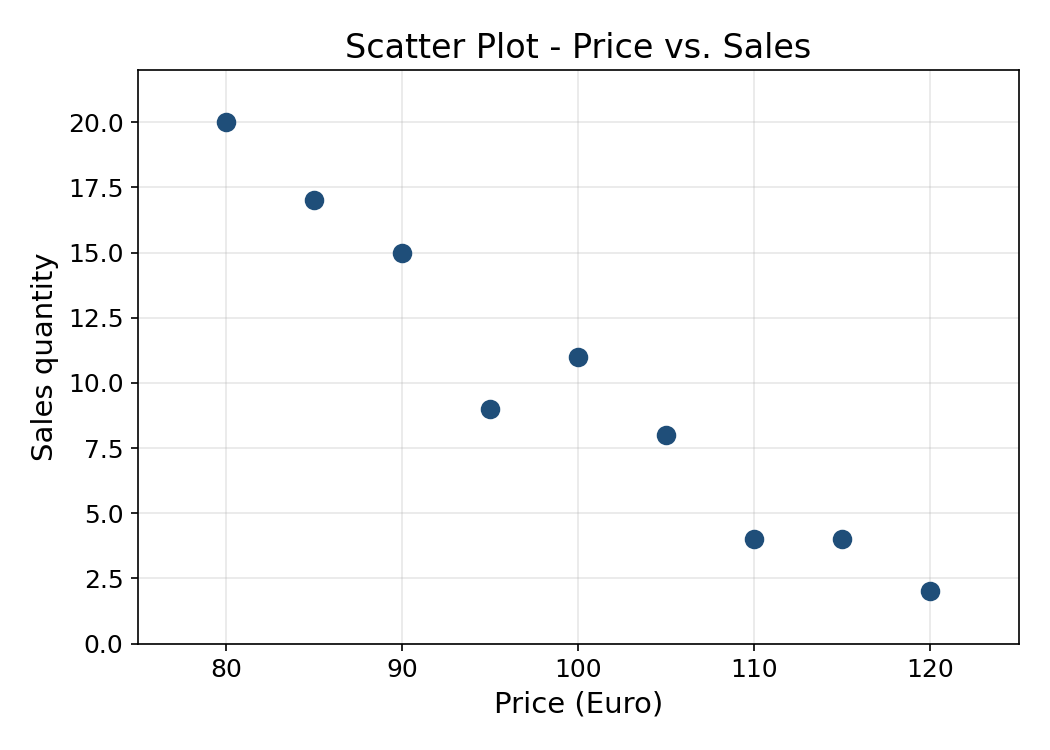
\includegraphics[width=0.8\textwidth,height=0.75\textheight,keepaspectratio]{images/image_020_en.png}
  \end{center}
\end{frame}

\subsection{Covariance and correlation}

\begin{frame}{Covariance}
  \begin{block}{Idea}
    The \emph{covariance} $s_{xy}$ measures the
    \textbf{joint variability} of two metric variables $X$ and $Y$.
  \end{block}

  \begin{block}{Computation (sample covariance)}
    \[
      s_{xy} \;=\; \operatorname{Cov}(X, Y)
             \;=\; \frac{1}{n-1} \sum_{i=1}^{n}
                   (x_i - \bar{x})(y_i - \bar{y})
    \]
    with range $\; -\infty < s_{xy} < +\infty$.
  \end{block}
  \inworten{Same divisor $n-1$ as the sample variance of Part~1 -- in fact
  $s_{xx}=s_x^2$: the covariance of a variable with itself is its
  variance.}
\end{frame}

\begin{frame}{Covariance -- interpretation}
  \begin{block}{Sign indicates the direction of the relationship}
    \begin{description}
      \item[$s_{xy} > 0$] \textbf{Positive (concordant) relationship.}
            Larger values of $X$ tend to go together with larger values
            of $Y$.
      \item[$s_{xy} < 0$] \textbf{Negative (discordant) relationship.}
            Larger values of $X$ tend to go together with smaller values
            of $Y$.
      \item[$s_{xy} = 0$] \textbf{No linear relationship.}
            The cloud of points shows no recognisable linear structure.
    \end{description}
  \end{block}

  \begin{alertblock}{Magnitude not directly interpretable}
    The covariance $s_{xy}$ has the unit ``unit of $X$ $\cdot$ unit of
    $Y$'' and depends on the scaling of the data.
  \end{alertblock}
\end{frame}

\begin{frame}{Correlation coefficient}
  \begin{block}{Idea}
    The correlation coefficient $r_{xy}$ is a
    \textbf{normalised covariance}: it measures the strength and
    direction of the \emph{linear} relationship between $X$ and $Y$
    -- \emph{independent of the units of measurement}.
  \end{block}

  \begin{block}{Computation}
    \[
      r_{xy} \;=\; \frac{s_{xy}}{s_x \, s_y}
             \;=\; \operatorname{Cov}\!\left(
                     \frac{X-\bar{x}}{s_x},\;
                     \frac{Y-\bar{y}}{s_y}
                   \right)
      \qquad -1 \le r_{xy} \le +1 .
    \]
  \end{block}

  \begin{exampleblock}{Reading}
    $r_{xy}$ is the covariance of the \emph{$z$-standardised} variables.
    Dividing by $s_x s_y$ cancels out the units.
  \end{exampleblock}
\end{frame}

\begin{frame}{Correlation coefficient -- strength of the relationship}
  \begin{block}{What $r_{xy}$ measures}
    The correlation coefficient measures the \textbf{degree of linear
    dependence} between $X$ and $Y$: $r_{xy}=\pm1$ means that all points
    lie exactly on a straight line.
  \end{block}

  \medskip

  \begin{block}{Strength of the relationship (rule of thumb)}
    \begin{center}
      \renewcommand{\arraystretch}{1.2}
      \begin{tabular}{ll}
        \toprule
        \textbf{Range} & \textbf{Interpretation} \\
        \midrule
        $|r_{xy}| > 0.8$               & strong correlation \\
        $0.5 \le |r_{xy}| \le 0.8$     & moderate correlation \\
        $|r_{xy}| < 0.5$               & weak correlation \\
        \bottomrule
      \end{tabular}
    \end{center}
  \end{block}
\end{frame}

\begin{frame}{Covariance and correlation -- lamp example}
  \begin{center}
    \footnotesize
    \renewcommand{\arraystretch}{1.0}
    \begin{tabular}{l|rrrrrrrrr|r}
      \toprule
      $x_i$ & 80 & 85 & 90 & 95 & 100 & 105 & 110 & 115 & 120 & $\bar x=100$\\
      $y_i$ & 20 & 17 & 15 & 9 & 11 & 8 & 4 & 4 & 2 & $\bar y=10$\\
      \midrule
      $x_i-\bar x$ & $-20$ & $-15$ & $-10$ & $-5$ & $0$ & $5$ & $10$ & $15$ & $20$ & \\
      $y_i-\bar y$ & $10$ & $7$ & $5$ & $-1$ & $1$ & $-2$ & $-6$ & $-6$ & $-8$ & \\
      $(x_i-\bar x)(y_i-\bar y)$ & $-200$ & $-105$ & $-50$ & $5$ & $0$ & $-10$ & $-60$ & $-90$ & $-160$ & $\Sigma=-670$\\
      \bottomrule
    \end{tabular}
  \end{center}
  \begin{exampleblock}{Calculation}
    \[
      s_{xy}=\frac{-670}{8}=-83.75,\qquad
      s_x=\sqrt{\tfrac{1500}{8}}=13.6931,\qquad
      s_y=\sqrt{\tfrac{316}{8}}=6.2849
    \]
    \[
      r_{xy}=\frac{-83.75}{13.6931\cdot 6.2849}=\mathbf{-0.9732}
    \]
  \end{exampleblock}
  \inworten{A strong negative linear relationship: the higher the price,
  the fewer lamps are sold.}
\end{frame}

\begin{frame}{Correlation coefficient -- limitations}
  \begin{alertblock}{No causal relationship}
    From $r_{xy}$ alone one \emph{cannot} infer which variable is
    independent ($X$) and which is dependent ($Y$). Correlation is
    \textbf{symmetric}: $r_{xy} = r_{yx}$.
  \end{alertblock}

  \medskip

  \begin{alertblock}{Spurious correlation possible}
    $r_{xy}$ can be $\ne 0$ \textbf{without} a substantive
    relationship between $X$ and $Y$ -- e.g.\ when both variables are
    influenced by a common third variable (we return to this as
    \emph{confounding} in multiple regression).
  \end{alertblock}

  \medskip

  \begin{block}{Remember}
    A high value of $|r_{xy}|$ is a \emph{statistical finding},
    not a \emph{causal statement}.
  \end{block}
\end{frame}

\begin{frame}[fragile]{Covariance and correlation with R}
  \begin{block}{Data}
\begin{lstlisting}
price    <- c(80, 85, 90, 95, 100, 105, 110, 115, 120)
quantity <- c(20, 17, 15,  9,  11,   8,   4,   4,   2)
plot(price, quantity)            # scatter plot
\end{lstlisting}
  \end{block}
  \begin{block}{Covariance and correlation}
\begin{lstlisting}
cov(price, quantity)             # -83.75
cor(price, quantity)             # -0.9732 (Pearson is the default)
\end{lstlisting}
  \end{block}
\end{frame}

% ============================================================================
% SECTION 2: SIMPLE LINEAR REGRESSION
% ============================================================================
\section[Simple regression]{Simple Linear Regression}

\subsection{Least squares estimation}

\begin{frame}{Motivation}
  \begin{block}{The question}
    How can the \textbf{best-fitting line} through the cloud of points be
    determined?
  \end{block}
  \begin{itemize}\setlength{\itemsep}{4pt}
    \item The correlation tells us \emph{how strong} the linear relationship
          is -- but not \emph{by how much} $Y$ changes when $X$ changes.
    \item A straight line answers exactly this: its \textbf{slope} is the
          change in $Y$ per unit of $X$.
    \item Two questions follow: \emph{which} line do we pick -- and how
          \emph{certain} can we be about it (Section ``Inference'')?
  \end{itemize}
\end{frame}

\begin{frame}{The best line through the cloud of points}
  \begin{block}{Regression line}
    The linear relationship between $X$ and $Y$ that we are looking
    for is described by a straight line:
    \begin{center}
      $y \;=\; \beta_0 + \beta_1 \, x$
    \end{center}
    \begin{description}
      \item[$\beta_0$] \emph{Intercept} -- value of $y$ at $x=0$;
            without $\beta_0$ all lines would pass through the origin.
      \item[$\beta_1$] \emph{Slope} -- change in $y$ when $x$
            increases by one unit.
    \end{description}
  \end{block}

  \begin{exampleblock}{Estimation and naming}
    The coefficients $\beta_0$ and $\beta_1$ are \textbf{estimated}
    from the data. Since they appear only at power $1$,
    one speaks of \textbf{linear regression}.
  \end{exampleblock}
\end{frame}

\begin{frame}{The regression model}
  \begin{block}{Regression model with error term}
    Since the observations generally do not lie exactly on the line,
    \emph{deviations} occur:
    \[
      y_i \;=\; \underbrace{\beta_0 + \beta_1 \, x_i}_{\text{systematic part}}
            \;+\; \underbrace{u_i}_{\text{error term}},
      \qquad i=1,\dots,n .
    \]
    \begin{description}
      \item[$\beta_0 + \beta_1 x_i$] the share of $y_i$ explained by $x_i$,
      \item[$u_i$] the part of the $i$-th observation that is
            \emph{not} explained by $X$.
    \end{description}
  \end{block}

  \begin{alertblock}{Requirement for the error term}
    The $u_i$ should contain \textbf{no systematic
    information} about $Y$ any more -- everything that can be
    explained must already be in the linear part.
  \end{alertblock}
\end{frame}

\begin{frame}{Intuition: minimise the vertical mistakes}
  \begin{columns}[T]
    \begin{column}{0.50\textwidth}
      \textbf{Each line makes a mistake on each point.}
      For observation $i$, the mistake is the vertical distance
      between the point $y_i$ and the line above $x_i$: the
      \textbf{residual} $\hat u_i=y_i-\hat y_i$.\par\medskip
      \textbf{We pick the line that makes the total squared
      mistake as small as possible.}\par\medskip
      \inworten{Slide the line until the sum of the squared red segments
      is minimal.}
    \end{column}
    \begin{column}{0.46\textwidth}
      \begin{tikzpicture}[scale=0.88,>=Stealth]
        \draw[->] (-0.2,0) -- (5.6,0) node[right]{$x$};
        \draw[->] (0,-0.2) -- (0,4.2) node[above]{$y$};
        \draw[very thick,hsbirot] (0.2,0.525) -- (5.2,3.65)
              node[above left,black,font=\footnotesize]{$\hat y=\hat\beta_0+\hat\beta_1x$};
        \foreach \x/\y in {0.6/0.6, 1.5/2.0, 2.4/1.7, 3.2/3.0, 4.0/2.5, 4.6/3.6} {
          \pgfmathsetmacro\yhat{0.4 + 0.625*\x}
          \draw[hsbiorange!90!black, very thick] (\x, \y) -- (\x, \yhat);
          \fill[hsbiblaudunkel] (\x, \y) circle (2.2pt);
        }
        \node[hsbiorange!90!black, anchor=west,font=\footnotesize] at (4.05,1.6) {residual $\hat u_i$};
      \end{tikzpicture}
    \end{column}
  \end{columns}
\end{frame}

\begin{frame}{Method of least squares (OLS)}
  \begin{block}{Idea}
    We look for the line $\hat{y} = \hat{\beta}_0 + \hat{\beta}_1\,x$
    such that the sum of the \emph{squared} residuals is as small as
    possible (\emph{ordinary least squares}, OLS).
  \end{block}

  \begin{block}{Minimisation problem}
    \[
        \min_{\hat{\beta}_0,\,\hat{\beta}_1}
        \;\sum_{i=1}^{n} \hat{u}_i^{\,2}
        \;=\;
        \min_{\hat{\beta}_0,\,\hat{\beta}_1}
        \;\sum_{i=1}^{n}
        \bigl(y_i - \hat{\beta}_0 - \hat{\beta}_1 x_i\bigr)^{2}
    \]
    with residuals
    $\hat{u}_i = y_i - \hat{y}_i = y_i - \hat{\beta}_0 - \hat{\beta}_1 x_i$.
  \end{block}

  \begin{exampleblock}{Why squared?}
    \begin{itemize}
      \item Positive and negative deviations \emph{do not} cancel out
            (as for the variance in Part~1).
      \item Large deviations are penalised more heavily than small ones.
    \end{itemize}
  \end{exampleblock}
\end{frame}

\begin{frame}{Derivation (1/2): set the derivatives to zero}
  \small
  The sum of squared residuals
  $\mathrm{RSS}(\beta_0,\beta_1)=\sum_{i}(y_i-\beta_0-\beta_1x_i)^2$ is a
  ``bowl'' in $(\beta_0,\beta_1)$; at its minimum both partial derivatives
  vanish:
  \begin{align*}
    \frac{\partial\,\mathrm{RSS}}{\partial \beta_0}
      &= -2 \sum_{i=1}^n (y_i - \beta_0 - \beta_1 x_i) \stackrel{!}{=} 0
      && \rhd\ \text{\scriptsize divide by } -2n\\[2pt]
    \Longrightarrow\quad \bar y &= \hat\beta_0+\hat\beta_1\bar x
      \quad\Longleftrightarrow\quad \hat\beta_0=\bar y-\hat\beta_1\bar x .
  \end{align*}
  \inworten{The first condition already shows that the line passes through
  the \textbf{centroid} $(\bar x,\bar y)$ of the cloud of points -- and that
  the residuals sum to zero.}
\end{frame}

\begin{frame}{Derivation (2/2): the slope}
  \small
  \begin{align*}
    \frac{\partial\,\mathrm{RSS}}{\partial \beta_1}
      &= -2 \sum_{i=1}^n x_i\,(y_i - \beta_0 - \beta_1 x_i) \stackrel{!}{=} 0
      && \rhd\ \text{\scriptsize insert }\hat\beta_0\\[2pt]
    0 &= \sum_{i=1}^n x_i\bigl[(y_i-\bar y)-\hat\beta_1(x_i-\bar x)\bigr]
      && \rhd\ \text{\scriptsize use }\textstyle\sum_i(x_i-\bar x)=0\\[2pt]
    0 &= \sum_{i=1}^n (x_i-\bar x)(y_i-\bar y)-\hat\beta_1\sum_{i=1}^n(x_i-\bar x)^2
  \end{align*}
  \kernaussage{Least-squares estimators:
  \[
    \hat\beta_1=\frac{\sum_{i}(x_i-\bar x)(y_i-\bar y)}{\sum_{i}(x_i-\bar x)^2}
      =\frac{S_{xy}}{S_{xx}}=\frac{s_{xy}}{s_x^{2}},
    \qquad
    \hat\beta_0=\bar y-\hat\beta_1\,\bar x .
  \]}
\end{frame}

\begin{frame}{Least squares solution}
  \begin{block}{Slope}
    \[
        \hat{\beta}_1 \;=\; \frac{s_{xy}}{s_x^{\,2}}
    \]
    The ratio of the \emph{covariance} of $X$ and $Y$ to the
    \emph{variance} of $X$.
  \end{block}

  \begin{block}{Intercept}
    \[
        \hat{\beta}_0 \;=\; \bar{y} - \hat{\beta}_1 \, \bar{x}
    \]
    Chosen so that the regression line passes through the
    \emph{centroid} $(\bar{x}, \bar{y})$ of the cloud of points.
  \end{block}
  \inworten{Estimated values are marked with a ``hat'': $\hat y_i$,
  $\hat\beta_0$, $\hat\beta_1$, $\hat u_i$.}
\end{frame}

\begin{frame}{Least squares solution -- interpretation}
  \begin{exampleblock}{Properties of the slope $\hat{\beta}_1$}
    \begin{itemize}
      \item $\hat{\beta}_1$ inherits the \textbf{sign} of the
            covariance $s_{xy}$.
      \item The slope is exactly $0$ if and only if $X$ and $Y$
            are \textbf{uncorrelated} ($s_{xy} = 0$).
      \item Connection to the correlation coefficient:
            \[
                \hat{\beta}_1 \;=\; r_{xy} \cdot \frac{s_y}{s_x}
            \]
    \end{itemize}
  \end{exampleblock}

  \begin{block}{Remember}
    Regression, correlation and covariance are closely related: the
    signs agree, and the slope differs from $r_{xy}$ only by the
    ratio of standard deviations $s_y / s_x$.
  \end{block}
\end{frame}

\begin{frame}{Least squares -- lamp example (calculation)}
  \textbf{From the table of the correlation example:} $\bar x=100$,
  $\bar y=10$, $S_{xy}=-670$, $S_{xx}=1500$.
  \begin{exampleblock}{Calculation}
    \begin{align*}
      \hat\beta_1 &= \frac{S_{xy}}{S_{xx}}=\frac{-670}{1500}=\mathbf{-0.4467}
        \qquad\Bigl(=\frac{s_{xy}}{s_x^2}=\frac{-83.75}{187.5}\Bigr)\\[4pt]
      \hat\beta_0 &= \bar y-\hat\beta_1\bar x = 10-(-0.4467)\cdot 100
                   = 10+44.67=\mathbf{54.67}
    \end{align*}
  \end{exampleblock}
  \begin{block}{Estimated regression line}
    \[
      \hat y_i = 54.67-0.4467\,x_i
    \]
  \end{block}
  \inworten{Check: $\hat\beta_1=r_{xy}\,s_y/s_x=-0.9732\cdot 6.2849/13.6931=-0.4467$
  \checkmark}
\end{frame}

\begin{frame}{Least squares -- lamp example (graph)}
  \begin{center}
    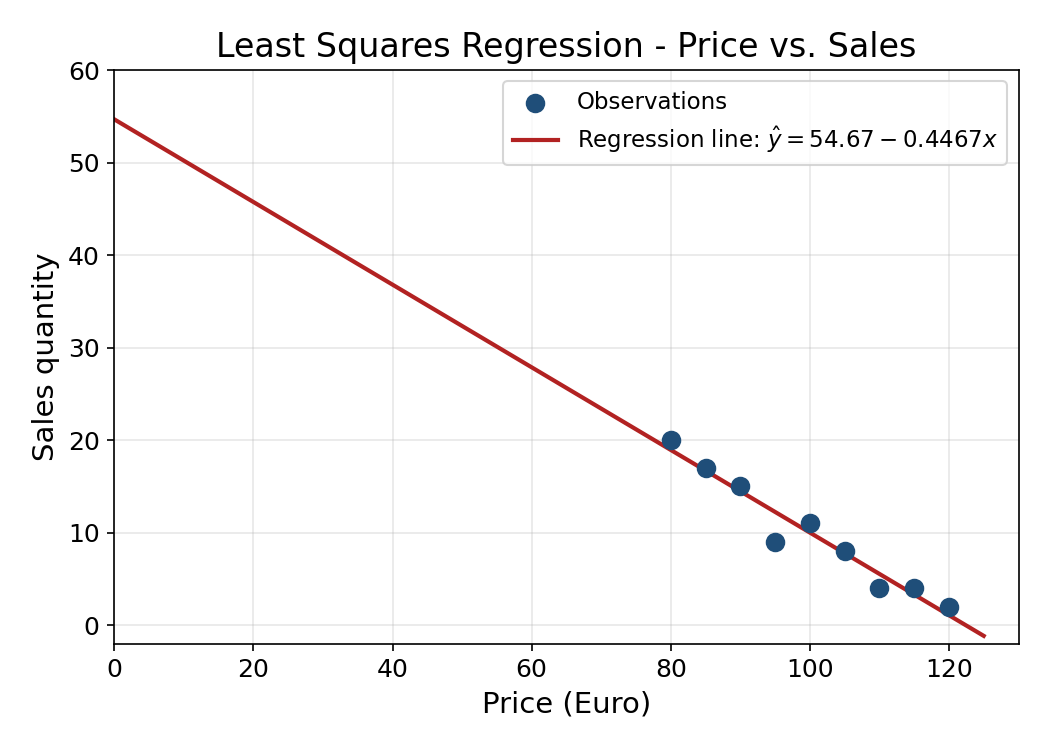
\includegraphics[width=0.8\textwidth,height=0.75\textheight,keepaspectratio]{images/image_021_en.png}
  \end{center}
\end{frame}

\begin{frame}{Example: interpretation of the slope}
  \begin{block}{Estimated regression line}
    \[
        \hat{y}_i \;=\; 54.67 \;-\; 0.4467 \cdot x_i
    \]
  \end{block}

  \begin{block}{Slope $\hat{\beta}_1 = -0.4467$}
    If the price increases by $1$ Euro, the sales quantity decreases
    \emph{on average} by $0.4467$ units -- or: a price increase of
    $10$ Euro costs about $4.5$ lamps.
  \end{block}

  \begin{exampleblock}{Economic interpretation}
    The negative sign confirms the expected \emph{inverse}
    relationship -- a classical downward-sloping
    \textbf{price-sales function}.
  \end{exampleblock}
\end{frame}

\begin{frame}{Example: intercept $\hat{\beta}_0 = 54.67$}
  \begin{block}{Formal meaning}
    Intersection of the regression line with the $y$-axis -- at a
    price of $0$ Euro one would compute sales of $54.67$ lamps.
  \end{block}

  \begin{alertblock}{Not meaningful in substantive terms}
    The value $x = 0$ lies far outside the observed price range
    ($80$ to $120$ Euro). The regression line is only
    reliable within the range of the data; outside the
    observed $x$-values (\emph{extrapolation}) extreme caution is
    required.
  \end{alertblock}
  \kernaussage{Interpret the slope as an average change \emph{within} the
  data range -- and the intercept only if $x=0$ is a meaningful value that
  lies near the data.}
\end{frame}

\begin{frame}[fragile]{Linear regression with R}
  \begin{block}{Coefficients by hand}
\begin{lstlisting}
(beta1 <- cov(price, quantity) / var(price))       # -0.4467
(beta0 <- mean(quantity) - beta1 * mean(price))    # 54.6667
beta1 * sd(price) / sd(quantity)                    # = cor(price, quantity)
\end{lstlisting}
  \end{block}

  \begin{block}{Regression with \texttt{lm()} (linear model)}
\begin{lstlisting}
reg <- lm(quantity ~ price)       # read: quantity explained by price
coef(reg)                         # 54.6667  -0.4467
plot(price, quantity, xlim = c(0, 125), ylim = c(0, 60))
abline(reg)
\end{lstlisting}
  \end{block}
\end{frame}

\subsection{Exercise}

\begin{frame}{Exercise -- least squares by hand}
  \begin{block}{Problem statement}
    Five observations are given:
    \[
      (x_i,y_i) = (1,3),\;(2,4),\;(3,2),\;(4,5),\;(5,6).
    \]
    \begin{enumerate}
      \item Compute the means $\bar x$ and $\bar y$.
      \item Compute $S_{xy}=\sum (x_i-\bar x)(y_i-\bar y)$ and
            $S_{xx}=\sum (x_i-\bar x)^2$, then $\hat\beta_1$ and
            $\hat\beta_0$.
      \item Write down the fitted line and predict $y$ at $x=6$.
      \item Interpret the slope in words.
    \end{enumerate}
  \end{block}
\end{frame}

\begin{frame}{Solution (1/2) -- least squares by hand}
  \textbf{(1) Means:} \
  $\bar x = \tfrac{1+2+3+4+5}{5}=3$, \quad
  $\bar y = \tfrac{3+4+2+5+6}{5}=4$.

  \medskip
  \textbf{(2) Deviations and sums:}
  \begin{center}
    \renewcommand{\arraystretch}{1.15}
    \begin{tabular}{l|rrrrr|r}
      \toprule
      $x_i-\bar x$ & $-2$ & $-1$ & $0$ & $1$ & $2$ & \\
      $y_i-\bar y$ & $-1$ & $0$ & $-2$ & $1$ & $2$ & \\
      \midrule
      $(x_i-\bar x)(y_i-\bar y)$ & $2$ & $0$ & $0$ & $1$ & $4$ & $S_{xy}=7$\\
      $(x_i-\bar x)^2$ & $4$ & $1$ & $0$ & $1$ & $4$ & $S_{xx}=10$\\
      \bottomrule
    \end{tabular}
  \end{center}
  \begin{exampleblock}{Estimates}
    \[
      \hat\beta_1 = \frac{7}{10}=\mathbf{0.7},\qquad
      \hat\beta_0 = \bar y - \hat\beta_1\bar x = 4-0.7\cdot 3 = \mathbf{1.9}.
    \]
  \end{exampleblock}
\end{frame}

\begin{frame}{Solution (2/2) -- least squares by hand}
  \textbf{(3) Fitted line and prediction:}
  \[
    \hat y = 1.9 + 0.7\,x, \qquad
    \hat y(6) = 1.9 + 0.7\cdot 6 = 6.1 .
  \]
  Check: at $x=\bar x=3$, $\hat y = 1.9+2.1 = 4 = \bar y$
  \checkmark\ (the line passes through the centroid).

  \medskip
  \textbf{(4) Interpretation:} a one-unit increase in $x$ goes along with
  an \emph{average} increase of $0.7$ units in $y$.
  \begin{alertblock}{Careful}
    $x=6$ lies outside the observed range $[1,5]$ -- the prediction
    $6.1$ is an (mild) \textbf{extrapolation} and less trustworthy than a
    prediction inside the data range.
  \end{alertblock}
\end{frame}

\subsection{Leverage values}

\begin{frame}{Method of least squares -- leverage values}
  \begin{alertblock}{Disadvantage of the method}
    Single points lying far away from the centre of the data cloud
    (e.g.\ measurement errors or \emph{outliers}) can exert a strong
    influence on the regression line -- the deviations enter the
    estimation \emph{squared}.
  \end{alertblock}

  \begin{block}{Leverage value $h_i$}
    The leverage value measures how \textbf{unusual} the $x$-value of
    observation $i$ is -- and thus how strongly this point can pull the
    line towards itself:
    \[
        h_i \;=\; \frac{1}{n} \;+\;
        \frac{(x_i - \bar{x})^{2}}{\sum_{j=1}^{n}(x_j - \bar{x})^{2}},
        \qquad \frac1n\le h_i\le 1 .
    \]
  \end{block}

  \inworten{The further $x_i$ lies from the mean $\bar{x}$, the larger
  $h_i$ becomes (a long ``lever arm'').}
\end{frame}

\begin{frame}{Leverage values -- rule of thumb}
  \begin{alertblock}{Rule of thumb for points with high leverage}
    \begin{description}
      \item[Simple regression] Values with $h_i > \dfrac{4}{n}$ are
            \textbf{flagged} as high-leverage points.
      \item[Small samples] Stricter threshold $h_i > \dfrac{6}{n}$.
    \end{description}
    (In multiple regression with $p$ explanatory variables:
    $h_i>2(p+1)/n$ -- see the section ``Diagnostics''.)
  \end{alertblock}

  \begin{exampleblock}{Caution}
    A flagged point is a reason to \textbf{inspect} it (measurement error?
    special case?) and to compare the fit with and without it -- not to
    delete it automatically. Every removal changes the estimate and must be
    justified \emph{substantively}.
  \end{exampleblock}
\end{frame}

\begin{frame}{Leverage values -- lamp example}
  $n=9$, $\bar x=100$, $S_{xx}=1500$:
  \begin{center}
    \renewcommand{\arraystretch}{1.2}
    \begin{tabular}{l|rrrrrrrrr}
      \toprule
      $x_i$ & 80 & 85 & 90 & 95 & 100 & 105 & 110 & 115 & 120 \\
      \midrule
      $h_i$ & $0.378$ & $0.261$ & $0.178$ & $0.128$ & $0.111$ & $0.128$ & $0.178$ & $0.261$ & $0.378$ \\
      \bottomrule
    \end{tabular}
  \end{center}
  \begin{exampleblock}{Calculation for the first store}
    \[
      h_1=\frac19+\frac{(80-100)^2}{1500}=0.1111+0.2667=0.378
    \]
  \end{exampleblock}
  \begin{block}{Assessment}
    Threshold $4/n=0.444$: no store has a high leverage -- the prices are
    spread evenly; the extreme prices $80$ and $120$ have the largest (but
    still harmless) influence.
  \end{block}
\end{frame}

% ============================================================================
% SECTION 3: GOODNESS OF FIT
% ============================================================================
\section[Fit]{Goodness of Fit: the Coefficient of Determination}

\subsection{Variance decomposition}

\begin{frame}{Variance decomposition}
  \begin{block}{Idea}
    The regression decomposes the variance $s_y^{\,2}$ into a
    variance \emph{on} the regression line $s_{\hat{y}}^{\,2}$ and a
    variance \emph{around} the regression line $s_{\hat{u}}^{\,2}$
    (the \textbf{residual variance}).
  \end{block}

  \begin{exampleblock}{Variance decomposition}
    \[
      s_y^{\,2} \;=\; s_{\hat{y}}^{\,2} \;+\; s_{\hat{u}}^{\,2}
    \]
    This decomposition is also called \textbf{analysis of variance (ANOVA)}.
  \end{exampleblock}

  \begin{block}{In words}
    (total variance of $y$) $=$ (variance explained by the regression)
    $+$ (residual variance)
  \end{block}
\end{frame}

\begin{frame}{Variance decomposition -- sums of squares}
  \begin{block}{Sum-of-squares decomposition}
    \[
        \underbrace{\sum_{i=1}^{n} (y_i - \bar{y})^2}_{\text{TSS (total)}}
        \;=\;
        \underbrace{\sum_{i=1}^{n} (\hat{y}_i - \bar{y})^2}_{\text{ESS (explained)}}
        \;+\;
        \underbrace{\sum_{i=1}^{n} \hat{u}_i^{\,2}}_{\text{RSS (residual)}}
    \]
  \end{block}

  \begin{exampleblock}{In variances}
    Dividing all three sums by $n-1$ gives the decomposition of variances
    $s_y^{\,2} = s_{\hat{y}}^{\,2} + s_{\hat{u}}^{\,2}$
    (the fitted values have mean $\bar y$, the residuals mean $0$):
    \begin{description}
      \item[$s_y^{\,2}$] total variance of $y$,
      \item[$s_{\hat{y}}^{\,2}$] variance \emph{explained} by the regression,
      \item[$s_{\hat{u}}^{\,2}$] \emph{residual variance} (unexplained part).
    \end{description}
  \end{exampleblock}
\end{frame}

\begin{frame}{Variance decomposition -- link to the method of least squares}
  \begin{block}{Starting point}
    The variance \emph{around} the regression line is the part of
    the total variance that cannot be explained by the regression.
    The coefficients are computed by \textbf{minimising exactly this
    residual variance} (least squares). Therefore it is \textbf{minimal}.
  \end{block}

  \begin{exampleblock}{Consequence for the variance decomposition}
    \[
        \underbrace{s_y^{\,2}}_{\text{fixed}}
        \;=\;
        \underbrace{s_{\hat{y}}^{\,2}}_{\text{\color{hsbigruen}maximal}}
        \;+\;
        \underbrace{s_{\hat{u}}^{\,2}}_{\text{\color{hsbirot}minimal}}
    \]
    $\Rightarrow$ No other straight line explains a larger share of the
    variance of $y$ than the least-squares line.
  \end{exampleblock}
\end{frame}

\subsection{Coefficient of determination}

\begin{frame}{Coefficient of determination}
  \begin{block}{Definition}
    The \textbf{coefficient of determination} $R^{2}$ is the ratio
    of the variance on the regression line to the total variance:
    \[
        R^{2} \;=\; \frac{s_{\hat{y}}^{\,2}}{s_y^{\,2}}
              \;=\; \frac{\text{ESS}}{\text{TSS}}
              \;=\; 1-\frac{\text{RSS}}{\text{TSS}}
        \qquad 0 \le R^{2} \le 1.
    \]
  \end{block}

  \begin{exampleblock}{Interpretation}
    The coefficient of determination gives the \emph{share} of the
    total variance of $y$ that is explained by the regression.
  \end{exampleblock}
\end{frame}

\begin{frame}{Coefficient of determination -- extreme cases}
  \begin{block}{$R^{2} = 1$: perfect fit}
    The regression explains the \emph{entire} variance of $y$.
    \textbf{All points lie exactly on the regression line}; all
    residuals are zero: $s_{\hat{u}}^{\,2} = 0$.
  \end{block}

  \begin{alertblock}{$R^{2} = 0$: no explained variance}
    The regression line explains no variance: $s_{\hat{y}}^{\,2} = 0$.
    \textbf{The regression line has zero slope}
    ($\hat{\beta}_1 = 0$) and runs at the level of the mean $\bar{y}$.
  \end{alertblock}

  \begin{exampleblock}{Rule of thumb}
    The closer $R^{2}$ is to $1$, the better the linear model
    explains the data. A low $R^{2}$ does \emph{not} mean that $X$
    and $Y$ are independent -- only that the \emph{linear}
    relationship is weak.
  \end{exampleblock}
\end{frame}

\begin{frame}{Explained variance -- derivation}
  \small
  \begin{block}{Step 1: mean of the fitted values}
    Since $\hat{\beta}_0$ and $\hat{\beta}_1$ are constants:
    $\;\bar{\hat{y}} = \tfrac{1}{n}\sum_{i}\hat{y}_i = \hat{\beta}_0 + \hat{\beta}_1\,\bar{x}\;(=\bar y)$.
  \end{block}

  \begin{block}{Step 2: form the difference -- the intercept cancels out}
    \[
      \hat{y}_i - \bar{\hat{y}}
        = \bigl(\hat{\beta}_0 + \hat{\beta}_1 x_i\bigr)
            - \bigl(\hat{\beta}_0 + \hat{\beta}_1 \bar{x}\bigr)
        = \hat{\beta}_1\,(x_i - \bar{x}).
    \]
  \end{block}

  \begin{block}{Step 3: square, sum, divide by $n-1$}
    \[
      s_{\hat{y}}^{\,2}
        = \tfrac{1}{n-1}\sum_{i=1}^{n}\hat{\beta}_1^{\,2}(x_i - \bar{x})^{2}
        = \hat{\beta}_1^{\,2}\cdot
              \underbrace{\tfrac{1}{n-1}\sum_{i=1}^{n}(x_i - \bar{x})^{2}}_{=\,s_x^{\,2}}
        = \hat{\beta}_1^{\,2}\, s_x^{\,2}.
    \]
  \end{block}
  \inworten{The explained variance is the variance of $x$, scaled by the
  \textbf{square} of the slope.}
\end{frame}

\begin{frame}{Coefficient of determination in simple regression}
  \begin{block}{Alternative formula}
    Substituting $s_{\hat{y}}^{\,2} = \hat{\beta}_1^{\,2}\, s_x^{\,2}$ into
    $R^2=s_{\hat{y}}^{\,2}/s_y^{\,2}$:
    \[
        R^{2} \;=\; \hat{\beta}_1^{\,2}\,\frac{s_x^{\,2}}{s_y^{\,2}}
              \;=\; \left(\hat\beta_1\frac{s_x}{s_y}\right)^{2}
              \;=\; \left(\frac{s_{xy}}{s_x\,s_y}\right)^{2}
              \;=\; r_{xy}^{2}.
    \]
  \end{block}

  \begin{exampleblock}{Root relation}
    $\sqrt{R^{2}} = |r_{xy}|$: the square root of $R^2$ is the
    \textbf{absolute value} of the correlation coefficient -- the sign
    (direction) is lost and must be read from $\hat\beta_1$ or $r_{xy}$.
  \end{exampleblock}

  \begin{alertblock}{Only valid in simple regression}
    With several explanatory variables, $R^2$ is no longer the square of a
    single correlation coefficient.
  \end{alertblock}
\end{frame}

\begin{frame}{Coefficient of determination -- lamp example}
  \begin{exampleblock}{Via the sums of squares}
    \[
      \text{TSS}=\sum(y_i-\bar y)^2=316,\qquad
      \text{RSS}=\sum\hat u_i^{\,2}=16.733,\qquad
      \text{ESS}=316-16.733=299.267
    \]
    \[
      R^2 = 1-\frac{16.733}{316}=\frac{299.267}{316}=\mathbf{0.9470}
    \]
  \end{exampleblock}
  \begin{block}{Cross-checks}
    \[
      R^2=\hat\beta_1^{\,2}\frac{s_x^2}{s_y^2}=(-0.4467)^2\cdot\frac{187.5}{39.5}=0.9470,
      \qquad R^2=r_{xy}^2=(-0.9732)^2=0.9470\ \checkmark
    \]
  \end{block}
  \inworten{About $95\,\%$ of the variation of the sales quantity across the
  stores is explained by the price.}
\end{frame}

\begin{frame}{Coefficient of determination -- assessment}
  \inworten{Because $R^2=r_{xy}^2$, a correlation that looks high gives a
  much smaller $R^2$: $r_{xy}=0.7$ yields only $R^2=0.49$.}

  \begin{exampleblock}{Rule of thumb (used in this course)}
    \begin{center}
    \begin{tabular}{ll}
      \toprule
      \textbf{Value of $R^{2}$} & \textbf{Assessment} \\
      \midrule
      $R^{2} < 0.6$           & weak fit \\
      $0.6 \le R^{2} < 0.8$   & moderate fit \\
      $R^{2} \ge 0.8$         & good fit \\
      \bottomrule
    \end{tabular}
    \end{center}
  \end{exampleblock}
  \begin{alertblock}{Context matters}
    What counts as ``good'' depends on the field: in finance or the social
    sciences an $R^2$ of $0.1$ can be valuable, in physics $0.95$ may be poor.
  \end{alertblock}
\end{frame}

\begin{frame}{Common misinterpretations of $R^2$}
  \begin{columns}[T]
    \begin{column}{0.48\textwidth}
      \begin{alertblock}{A high $R^2$ does \emph{not} prove}
        \begin{itemize}
          \item that the model is \emph{correct} (a curved relationship
                can still give a high $R^2$),
          \item that $X$ \emph{causes} $Y$,
          \item that predictions \emph{outside} the data range are good.
        \end{itemize}
      \end{alertblock}
    \end{column}
    \begin{column}{0.48\textwidth}
      \begin{alertblock}{A low $R^2$ does \emph{not} prove}
        \begin{itemize}
          \item that the model is \emph{useless},
          \item that $X$ is \emph{irrelevant} -- the slope can still be
                clearly different from zero (see the $t$-test later),
          \item that there is no \emph{other} relationship.
        \end{itemize}
      \end{alertblock}
    \end{column}
  \end{columns}
  \kernaussage{Never judge a regression by $R^2$ alone -- always look at the
  residual plot and at the uncertainty of the coefficients.}
\end{frame}

\subsection{Useful transformations}

\begin{frame}{Useful transformations of the formulas}
  \begin{block}{Goal}
    The relationships between \textbf{correlation coefficient},
    \textbf{slope} $\hat{\beta}_1$ and \textbf{coefficient of
    determination} $R^{2}$ greatly simplify calculations by hand -- in
    particular because the factors $\tfrac{1}{n-1}$ \emph{cancel}.
  \end{block}

  \begin{exampleblock}{Overview}
    \begin{align*}
      r_{xy} &= \frac{S_{xy}}{\sqrt{S_{xx}}\,\sqrt{S_{yy}}}, &
      \hat\beta_1 &= \frac{S_{xy}}{S_{xx}}, &
      R^2 &= r_{xy}^2=\frac{S_{xy}^2}{S_{xx}\,S_{yy}}
    \end{align*}
    with the plain sums $S_{xx}=\sum(x_i-\bar x)^2$,
    $S_{yy}=\sum(y_i-\bar y)^2$, $S_{xy}=\sum(x_i-\bar x)(y_i-\bar y)$.
  \end{exampleblock}
\end{frame}

\begin{frame}{Correlation coefficient -- cancelling the prefactor}
  \begin{block}{Starting formula}
    \[
        r_{xy} \;=\; \frac{s_{xy}}{s_x\,s_y}
        \;=\; \frac{\tfrac{1}{n-1}S_{xy}}
                    {\sqrt{\tfrac{1}{n-1}S_{xx}}
                     \cdot
                     \sqrt{\tfrac{1}{n-1}S_{yy}}}
    \]
  \end{block}

  \begin{exampleblock}{Combining the roots}
    \[
        \sqrt{\tfrac{1}{n-1}\,A} \cdot \sqrt{\tfrac{1}{n-1}\,B}
        \;=\; \tfrac{1}{n-1}\sqrt{A\,B}
        \quad\Longrightarrow\quad
        r_{xy}=\frac{S_{xy}}{\sqrt{S_{xx}\,S_{yy}}} .
    \]
  \end{exampleblock}

  \begin{alertblock}{Remember}
    The factor $\tfrac{1}{n-1}$ appears in numerator \emph{and}
    denominator -- it can be omitted. The same holds for
    $\hat\beta_1=s_{xy}/s_x^2=S_{xy}/S_{xx}$.
  \end{alertblock}
\end{frame}

\begin{frame}{Coefficient of determination -- via the residuals}
  \begin{block}{Three equivalent formulas}
    \[
        R^{2} \;=\; \frac{\sum_{i}(\hat{y}_i - \bar{y})^{2}}
                         {\sum_{i}(y_i - \bar{y})^{2}}
        \;=\; 1 - \frac{\sum_{i}(y_i - \hat{y}_i)^{2}}
                        {\sum_{i}(y_i - \bar{y})^{2}}
        \;=\; r_{xy}^2 \quad\text{(simple regression)}
    \]
  \end{block}

  \begin{exampleblock}{In words}
    \[
        R^{2} \;=\; 1 - \frac{\text{sum of squared residuals}}
        {\text{sum of squared deviations of $y$ from the mean}}
    \]
  \end{exampleblock}
  \inworten{The middle formula is the one that also works in multiple
  regression -- it is the one \texttt{R} uses.}
\end{frame}

\begin{frame}[fragile]{Coefficient of determination in R}
  \begin{block}{R command}
\begin{lstlisting}
summary(reg)                   # full output, incl. "Multiple R-squared"
summary(reg)$r.squared         # 0.9470
\end{lstlisting}
  \end{block}

  \begin{exampleblock}{Manual variants}
\begin{lstlisting}
RSS <- sum(resid(reg)^2)                       # 16.7333
TSS <- sum((quantity - mean(quantity))^2)      # 316
1 - RSS / TSS                                  # 0.9470
cor(price, quantity)^2                         # simple regression only
\end{lstlisting}
  \end{exampleblock}
\end{frame}

\subsection{Exercise}

\begin{frame}{Exercise -- $R^2$ and the residual sum of squares}
  \begin{block}{Problem statement}
    For the five points of the exercise ``least squares by hand''
    ($\hat y=1.9+0.7x$) we have $S_{xx}=10$, $S_{xy}=7$ and
    $S_{yy}=\text{TSS}=10$.
    \begin{enumerate}
      \item Compute the correlation coefficient $r_{xy}$.
      \item Compute the fitted values, the residuals and RSS.
      \item Compute $R^2$ in two ways and interpret it.
    \end{enumerate}
  \end{block}
\end{frame}

\begin{frame}{Solution (1/2) -- $R^2$ and the residual sum of squares}
  \textbf{(1) Correlation:}
  $\;r_{xy}=\dfrac{S_{xy}}{\sqrt{S_{xx}S_{yy}}}=\dfrac{7}{\sqrt{10\cdot10}}=\mathbf{0.7}$.

  \medskip
  \textbf{(2) Fitted values and residuals} ($\hat y_i=1.9+0.7x_i$):
  \begin{center}
    \renewcommand{\arraystretch}{1.15}
    \begin{tabular}{l|rrrrr|r}
      \toprule
      $y_i$ & $3$ & $4$ & $2$ & $5$ & $6$ & \\
      $\hat y_i$ & $2.6$ & $3.3$ & $4.0$ & $4.7$ & $5.4$ & \\
      $\hat u_i$ & $0.4$ & $0.7$ & $-2.0$ & $0.3$ & $0.6$ & $\Sigma=0$ \checkmark\\
      $\hat u_i^{\,2}$ & $0.16$ & $0.49$ & $4.00$ & $0.09$ & $0.36$ & $\text{RSS}=5.1$\\
      \bottomrule
    \end{tabular}
  \end{center}
  \inworten{The residuals sum to zero -- a property of every least-squares
  line with intercept.}
\end{frame}

\begin{frame}{Solution (2/2) -- $R^2$ and the residual sum of squares}
  \textbf{(3) Two ways to $R^2$:}
  \[
    R^2 = 1-\frac{\text{RSS}}{\text{TSS}} = 1-\frac{5.1}{10}=\mathbf{0.49},
    \qquad
    R^2=r_{xy}^2=0.7^2=0.49\ \checkmark
  \]
  \begin{exampleblock}{Interpretation}
    $49\,\%$ of the variance of $y$ is explained by $x$, $51\,\%$ remain
    unexplained: a \textbf{weak} fit -- although $r_{xy}=0.7$ looked
    ``moderate''.
  \end{exampleblock}
  \begin{alertblock}{Common mistake}
    Reading $R^2=0.49$ as ``$49\,\%$ of the points are predicted correctly''.
    $R^2$ is a share of \emph{variance}, not a hit rate.
  \end{alertblock}
\end{frame}

% ============================================================================
% SECTION 4: RESIDUAL ANALYSIS
% ============================================================================
\section[Residuals]{Residual Analysis}

\subsection{Assumptions and residual plot}

\begin{frame}{Assumptions on the error term}
  \begin{block}{Four standard assumptions}
    \begin{description}
      \setlength{\itemsep}{0.4em}
      \item[Expected value $0$]
            $E(u_i) = 0$ -- no systematic error on average.
      \item[Homoscedasticity]
            $\operatorname{Var}(u_i) = \sigma^{2}$ for all $i$ --
            \emph{constant} variance, independent of $x_i$.
      \item[No autocorrelation]
            $\operatorname{Cov}(u_i, u_j) = 0$ for $i \ne j$ --
            the errors are pairwise uncorrelated.
      \item[Normal distribution]
            $u_i \sim N(0, \sigma^{2})$ -- required for
            confidence intervals and hypothesis tests (Section ``Inference'').
    \end{description}
  \end{block}

  \begin{alertblock}{Important}
    The assumptions are \textbf{not self-evident} -- they have to be
    \textbf{checked}. We check them with the \emph{residuals}
    $\hat u_i$, our observable stand-ins for the unobservable errors $u_i$.
  \end{alertblock}
\end{frame}

\begin{frame}{Residuals -- required structure}
  \begin{block}{Basic principle}
    The residuals $\hat{u}_i$ should contain \textbf{no
    systematic structure}: in the residual plot no recognisable
    pattern should be visible. Any structure indicates that the
    model has \emph{not} explained something it should have explained.
  \end{block}

  \begin{alertblock}{Typical structures pointing to model errors}
    \begin{description}
      \item[Systematic patterns] indicate a \textbf{wrong model
            equation} (e.g.\ non-linear relationship, missing variable).
      \item[Autocorrelation] -- successive residuals are correlated
            ($\operatorname{Cov}(u_i,u_j) \ne 0$); typical for time series.
      \item[Heteroscedasticity] -- the spread of the residuals
            depends on $x_i$ ($\operatorname{Var}(u_i)$ not constant).
    \end{description}
  \end{alertblock}
\end{frame}

\begin{frame}{Residual plot}
  \begin{block}{Idea}
    A \emph{residual plot} displays the estimated residuals
    graphically in order to check the \textbf{structure of the
    deviations} from the regression line.
  \end{block}

  \begin{block}{Estimated residuals}
    \[
        \hat{u}_i \;=\; y_i - \hat{y}_i
                 \;=\; y_i - \bigl(\hat{\beta}_0 + \hat{\beta}_1 x_i\bigr)
    \]
  \end{block}

  \begin{block}{Layout of the plot}
    \textbf{$x$-axis:} fitted values $\hat{y}_i$ \qquad
    \textbf{$y$-axis:} residuals $\hat{u}_i$ \qquad
    (points $(\hat{y}_i,\, \hat{u}_i)$, $i = 1, \ldots, n$)
  \end{block}

  \begin{exampleblock}{What we want to see}
    A \emph{structureless} cloud of points around the zero line.
  \end{exampleblock}
\end{frame}

\begin{frame}{Residual plot -- pattern recognition}
  \begin{center}
    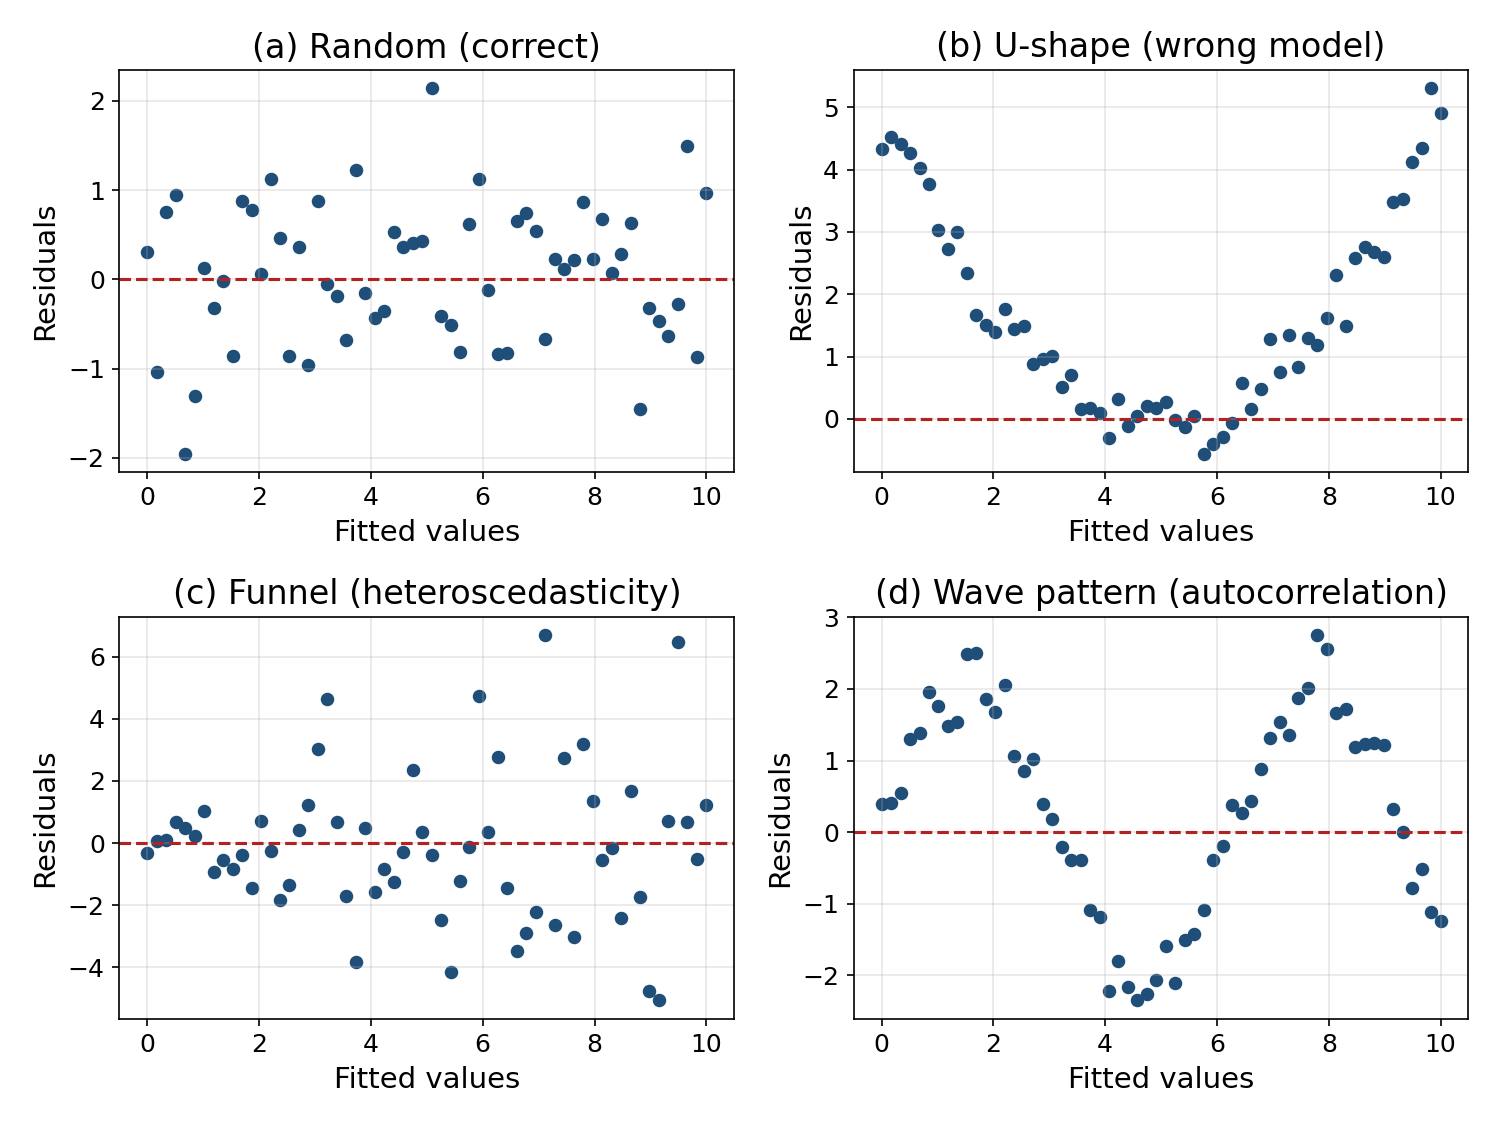
\includegraphics[width=0.9\textwidth,height=0.78\textheight,keepaspectratio]{images/image_022_en.png}
  \end{center}
\end{frame}

\begin{frame}{Residual plot -- lamp example}
  \begin{columns}[c]
    \begin{column}{0.62\textwidth}
      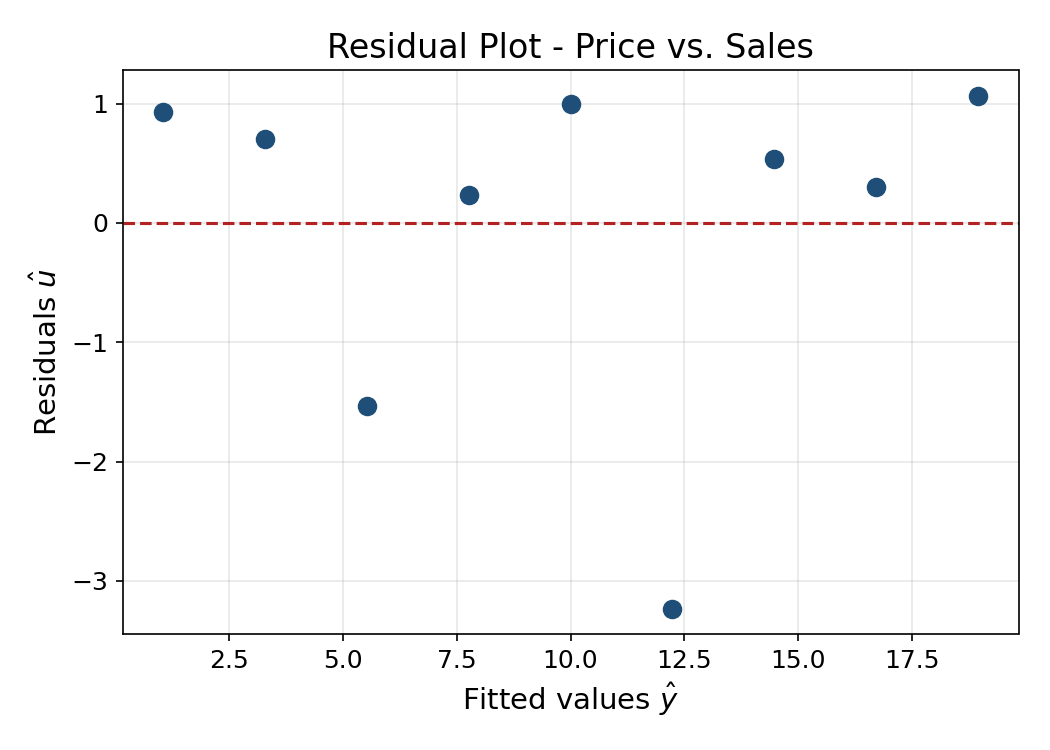
\includegraphics[width=\textwidth,height=0.74\textheight,keepaspectratio]{images/image_023_en.png}
    \end{column}
    \begin{column}{0.35\textwidth}
      \begin{exampleblock}{Observation}
        No systematic pattern visible -- the residuals scatter around
        zero without curvature or funnel shape.
      \end{exampleblock}
      \begin{alertblock}{But}
        One store ($x=95$, $\hat u_4=-3.23$) deviates clearly -- with
        $n=9$, single points weigh heavily.
      \end{alertblock}
    \end{column}
  \end{columns}
\end{frame}

\begin{frame}[fragile]{Creating a residual plot with R}
  \begin{block}{R commands}
\begin{lstlisting}
reg <- lm(quantity ~ price)
plot(fitted(reg), resid(reg), xlab = "fitted values",
     ylab = "residuals", main = "Residual plot")
abline(h = 0, lty = 2)        # zero line for orientation
\end{lstlisting}
  \end{block}

  \begin{block}{Helper functions}
    \begin{itemize}
      \item \texttt{fitted(reg)}: fitted values
            $\hat{y}_i = \hat{\beta}_0 + \hat{\beta}_1 x_i$ ($x$-axis)
      \item \texttt{resid(reg)}: residuals
            $\hat{u}_i = y_i - \hat{y}_i$ ($y$-axis)
    \end{itemize}
  \end{block}
\end{frame}

\subsection{QQ-plot}

\begin{frame}{QQ-plot}
  \begin{block}{Assumption}
    The errors of the linear regression are
    \textbf{normally distributed}.
  \end{block}

  \begin{exampleblock}{Tool for checking}
    Checking normality with the help of a \textbf{QQ-plot}
    (quantile-quantile plot).
  \end{exampleblock}
  \inworten{The normal distribution is the basis of the $t$-tests and
  confidence intervals for the coefficients -- exactly as in Part~3 for
  the mean.}
\end{frame}

\begin{frame}{What is a QQ-plot?}
  \begin{block}{Definition}
    The \emph{QQ-plot} is a \textbf{quantile-quantile graph}: the
    quantiles of two distributions are plotted against each other on
    the two axes.
  \end{block}

  \begin{block}{Layout and reference line}
    For better comparison a
    \textbf{line connecting the $25\,\%$ and the $75\,\%$ quantile}
    is drawn.
  \end{block}

  \begin{alertblock}{Interpretation}
    The further the points lie from the line,
    \textbf{the more dissimilar} the two distributions are. If all
    points lie on the line, the distributions have the same shape.
  \end{alertblock}
\end{frame}

\begin{frame}{What is a QQ-plot? -- example}
  \begin{block}{Lamp example}
    \begin{center}
      \begin{tabular}{lrrrrrrrrr}
        \toprule
        $x$ (price) & 80 & 85 & 90 & 95 & 100 & 105 & 110 & 115 & 120 \\
        $y$ (sales) & 20 & 17 & 15 & 9  & 11  & 8   & 4   & 4   & 2   \\
        \bottomrule
      \end{tabular}
    \end{center}
  \end{block}

  \begin{block}{Step 1 -- sort the data}
    For a QQ-plot, the $x$ and $y$ data are \textbf{sorted
    separately} (here -- and only here -- the pairs are broken up, because
    we compare two \emph{distributions}):
    \begin{center}
      \begin{tabular}{lrrrrrrrrr}
        \toprule
        $x^{\text{sort}}$ & 80 & 85 & 90 & 95 & 100 & 105 & 110 & 115 & 120 \\
        $y^{\text{sort}}$ & 2  & 4  & 4  & 8  & 9   & 11  & 15  & 17  & 20  \\
        \bottomrule
      \end{tabular}
    \end{center}
    The pairs $(x_{(i)}, y_{(i)})$ are then plotted.
  \end{block}
\end{frame}

\begin{frame}{What is a QQ-plot? -- example (graph)}
  \begin{center}
    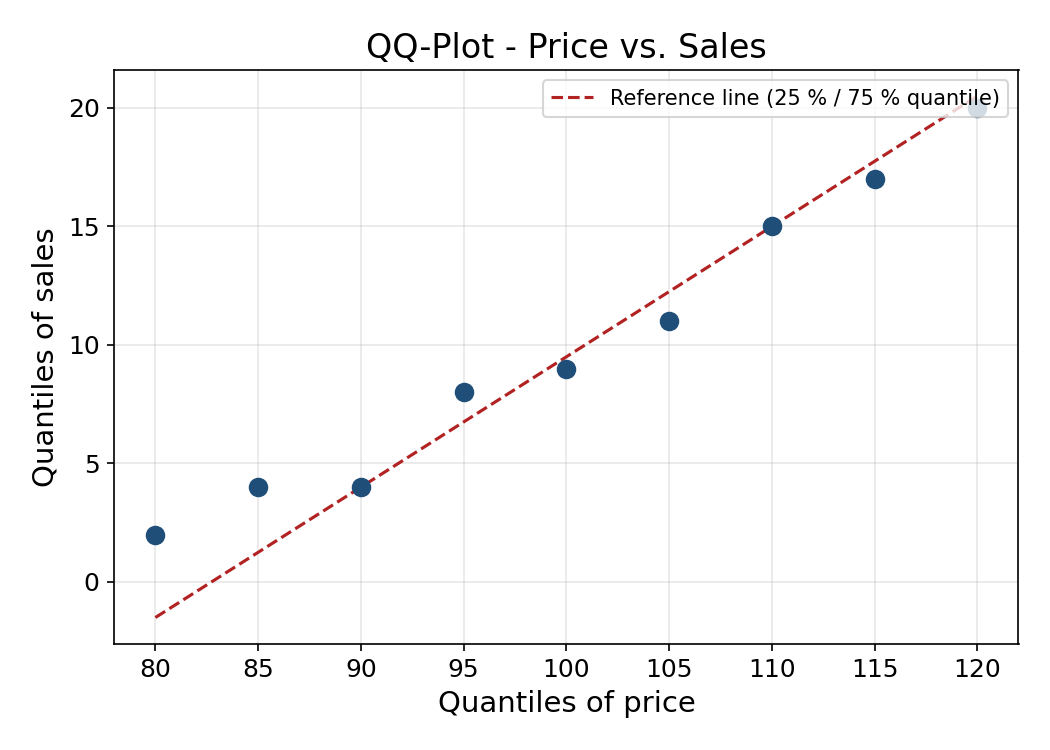
\includegraphics[width=0.85\textwidth,height=0.78\textheight,keepaspectratio]{images/image_024_en.png}
  \end{center}
\end{frame}

\begin{frame}[fragile]{Creating a QQ-plot with R}
  \begin{block}{Drawing the QQ-plot}
\begin{lstlisting}
qqplot(price, quantity)
\end{lstlisting}
  \end{block}

  \begin{block}{Adding a line to the QQ-plot}
\begin{lstlisting}
qqline(quantity,
       distribution = function(p) quantile(price, prob = p),
       lty = 2)
\end{lstlisting}
  \end{block}

  \begin{exampleblock}{Idea}
    \texttt{qqplot()} produces a QQ-diagram for the
    \emph{empirical} distributions of two samples;
    \texttt{qqline()} adds a reference line through the $25\,\%$
    and $75\,\%$ quantiles.
  \end{exampleblock}
\end{frame}

\begin{frame}{Inspecting the residuals with the QQ-plot}
  \begin{block}{QQ-plot sample vs.\ theory}
    The QQ-plot can also compare an empirical distribution with a
    \emph{theoretical} distribution -- here the residuals with the
    \textbf{standard normal distribution}.
  \end{block}

  \begin{block}{Construction}
    \begin{description}
      \item[$y$-axis] sorted residuals $\hat{u}_{(i)}$
      \item[$x$-axis] quantiles $z_i$ of the standard normal distribution
    \end{description}
    The theoretical quantiles are obtained from
    \[
        \Phi(z_i) \;=\; \frac{i - 0.5}{n},
        \qquad z_i = \Phi^{-1}\!\left(\tfrac{i-0.5}{n}\right).
    \]
  \end{block}
\end{frame}

\begin{frame}{Inspecting the residuals with the QQ-plot -- example}
  \begin{center}
    \scriptsize
    \renewcommand{\arraystretch}{1.1}
    \begin{tabular}{rrrrr}
      \toprule
      \textbf{Residual $\hat{u}_i$} & \textbf{$\hat{u}_{(i)}$ sorted} & \textbf{Index $i$} & \textbf{$\tfrac{i-0.5}{n}$} & \textbf{Quantile $z_i$} \\
      \midrule
       $1.0667$ & $-3.2333$ & 1 & $0.0556$ & $-1.5932$ \\
       $0.3000$ & $-1.5333$ & 2 & $0.1667$ & $-0.9674$ \\
       $0.5333$ &  $0.2333$ & 3 & $0.2778$ & $-0.5895$ \\
      $-3.2333$ &  $0.3000$ & 4 & $0.3889$ & $-0.2822$ \\
       $1.0000$ &  $0.5333$ & 5 & $0.5000$ &  $0.0000$ \\
       $0.2333$ &  $0.7000$ & 6 & $0.6111$ &  $0.2822$ \\
      $-1.5333$ &  $0.9333$ & 7 & $0.7222$ &  $0.5895$ \\
       $0.7000$ &  $1.0000$ & 8 & $0.8333$ &  $0.9674$ \\
       $0.9333$ &  $1.0667$ & 9 & $0.9444$ &  $1.5932$ \\
      \bottomrule
    \end{tabular}
  \end{center}
\end{frame}

\begin{frame}{Inspecting the residuals with the QQ-plot -- interpretation}
  \begin{columns}[T]
    \begin{column}{0.52\textwidth}
      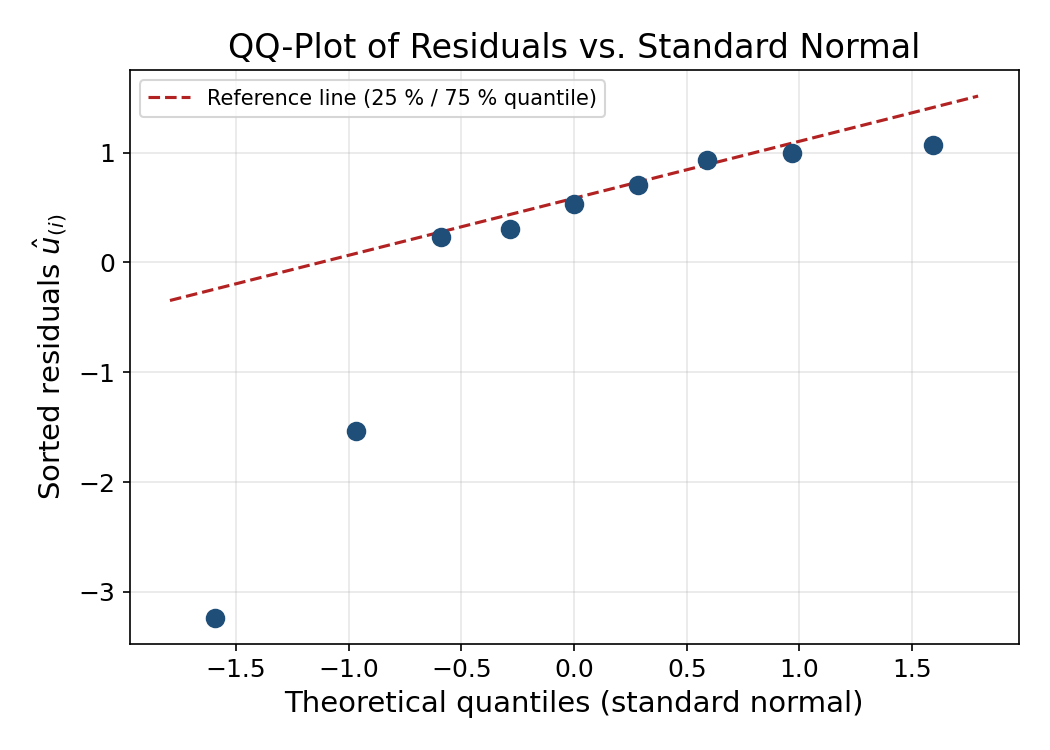
\includegraphics[width=\textwidth,height=0.76\textheight,keepaspectratio]{images/image_025_en.png}
    \end{column}
    \begin{column}{0.44\textwidth}
      \begin{block}{Observation}
        \textbf{In the middle} good fit to the normal distribution.
        \textbf{At the lower end} two residuals lie clearly below the line.
      \end{block}

      \begin{alertblock}{Conclusion}
        $n=9$ -- only very few data points! The normality assumption is
        \textbf{questionable}; tests and confidence intervals for this
        example should be read with caution.
      \end{alertblock}
    \end{column}
  \end{columns}
\end{frame}

\begin{frame}[fragile]{QQ-plot of the residuals against the normal distribution in R}
  \begin{block}{Create QQ-plot}
\begin{lstlisting}
qqnorm(resid(reg))
\end{lstlisting}
  \end{block}

  \begin{block}{Add line through the quartiles}
\begin{lstlisting}
qqline(resid(reg))
\end{lstlisting}
  \end{block}

  \begin{exampleblock}{What the commands do}
    \texttt{qqnorm()} computes the plotting positions
    $p_i = (i-0.5)/n$, the normal quantiles
    $z_i = \Phi^{-1}(p_i)$ and plots the pairs
    $(z_i, \hat{u}_{(i)})$. \texttt{qqline()} adds a reference
    line through the $25\,\%$ and $75\,\%$ quantiles.
  \end{exampleblock}
\end{frame}

\subsection{Exercises}

\begin{frame}{Exercise -- reading residual plots}
  \begin{block}{Problem statement}
    For each pattern in a residual plot (residuals against fitted values),
    name the problem and a possible remedy.
    \begin{enumerate}
      \item The residuals form a clear U-shape around zero.
      \item The residuals fan out into a funnel: small spread at low fitted
            values, large spread at high fitted values.
      \item The residuals form a random band of roughly constant width
            around zero.
      \item One point lies far away from all others in $x$-direction and
            pulls the line towards itself.
    \end{enumerate}
  \end{block}
\end{frame}

\begin{frame}{Solution -- reading residual plots}
  \begin{enumerate}\setlength{\itemsep}{4pt}
    \item \textbf{Non-linearity:} the straight line is the wrong model
          equation. \emph{Remedy:} add a quadratic term $x^2$ or transform
          $x$ (e.g.\ $\log x$).
    \item \textbf{Heteroscedasticity:} the variance of the errors is not
          constant -- standard errors and tests become unreliable.
          \emph{Remedy:} transform $y$ (e.g.\ $\log y$).
    \item \textbf{Everything fine:} the assumptions look satisfied -- no
          action needed.
    \item \textbf{High leverage point:} check $h_i$ against $4/n$; inspect
          the point and compare the fit with and without it.
  \end{enumerate}
  \begin{alertblock}{Common mistake}
    Judging the assumptions from $R^2$. A high $R^2$ can coexist with
    patterns 1, 2 and 4 -- only the residual plot reveals them.
  \end{alertblock}
\end{frame}

\begin{frame}{Exercise -- body heights and shoe sizes: overview}
  \begin{block}{Data basis}
    Body heights $k_i$ (in cm) and shoe sizes $s_i$ of $n = 15$ persons
    (the body heights are those of the exercise in Part~2):
    \begin{center}
      \small
      \begin{tabular}{l|*{15}{c}}
        \toprule
        $k_i$ & 164 & 162 & 168 & 198 & 166 & 166 & 192 & 160 & 151 & 175 & 180 & 160 & 168 & 175 & 168\\
        $s_i$ & 39 & 38 & 39 & 46 & 40 & 39 & 45 & 37 & 36 & 42 & 43 & 38 & 41 & 40 & 39\\
        \bottomrule
      \end{tabular}
    \end{center}
  \end{block}

  \begin{exampleblock}{Tasks}
    \begin{description}
      \setlength{\itemsep}{0.2em}
      \item[Task 1] Compute the \textbf{covariance} and the
            \textbf{correlation coefficient}.
      \item[Task 2] Estimate the regression $s_i = \beta_0 + \beta_1\, k_i + u_i$,
            draw the scatter plot with regression line and the residual
            plot, and compute $R^2$.
      \item[Task 3] Create and interpret a \textbf{QQ-plot} of the residuals.
    \end{description}
  \end{exampleblock}
\end{frame}

\begin{frame}{Solution Task 1 -- means and covariance}
  \begin{block}{Step 1: means}
    \[
      \bar{k} = \tfrac{1}{15}\sum_{i=1}^{15} k_i = \tfrac{2553}{15} = 170.2,
      \qquad
      \bar{s} = \tfrac{1}{15}\sum_{i=1}^{15} s_i = \tfrac{602}{15} = 40.1333
    \]
  \end{block}

  \begin{block}{Step 2: covariance}
    \[
      s_{ks}
        = \frac{1}{n-1}\sum_{i=1}^{n}(k_i - \bar{k})(s_i - \bar{s})
        = \frac{471.6}{14}
        = 33.6857
    \]
  \end{block}
  \inworten{Positive covariance: taller persons tend to have larger shoe
  sizes.}
\end{frame}

\begin{frame}{Solution Task 1 -- standard deviations and correlation}
  \begin{block}{Step 3: sample variances / standard deviations}
    \[
      s_k^{\,2} = \tfrac{2122.4}{14} = 151.6 \;\Rightarrow\; s_k = 12.3126,
      \qquad
      s_s^{\,2} = \tfrac{111.7333}{14} = 7.9810 \;\Rightarrow\; s_s = 2.8251
    \]
  \end{block}

  \begin{exampleblock}{Step 4: correlation coefficient}
    \[
      r_{ks} = \frac{s_{ks}}{s_k\,s_s}
        = \frac{33.6857}{12.3126 \cdot 2.8251}
        = \mathbf{0.9684}
    \]
  \end{exampleblock}

  \begin{alertblock}{Interpretation}
    Very strong positive linear relationship between body height
    and shoe size.
  \end{alertblock}
\end{frame}

\begin{frame}{Solution Task 2 -- regression coefficients}
  \begin{block}{Slope $\hat{\beta}_1$}
    \[
      \hat{\beta}_1 = \frac{s_{ks}}{s_k^{\,2}} = \frac{33.6857}{151.6}
        = \frac{471.6}{2122.4} = \mathbf{0.2222}
    \]
  \end{block}

  \begin{block}{Intercept $\hat{\beta}_0$}
    \[
      \hat{\beta}_0 = \bar{s} - \hat{\beta}_1\,\bar{k}
        = 40.1333 - 0.2222 \cdot 170.2 = \mathbf{2.3147}
    \]
  \end{block}

  \begin{exampleblock}{Estimated model}
    \[
      \hat{s}_i = 2.3147 + 0.2222\, k_i
    \]
    \emph{Per $1\,$cm of body height the shoe size increases on average by
    about $0.22$ -- i.e.\ by about one size per $4.5\,$cm.}
  \end{exampleblock}
\end{frame}

\begin{frame}{Solution Task 2 -- coefficient of determination $R^{2}$}
  \begin{block}{Via the alternative formula}
    \[
      R^{2} = \hat{\beta}_1^{\,2}\,\frac{s_k^{\,2}}{s_s^{\,2}}
        = (0.2222)^{2}\cdot\frac{151.6}{7.9810}
        = 0.9379
    \]
  \end{block}

  \begin{block}{Cross-check via $r_{ks}^{2}$}
    \[
      R^{2} = r_{ks}^{2} = (0.9684)^{2} = 0.9379 \quad\checkmark
    \]
  \end{block}

  \begin{alertblock}{Interpretation}
    About $93.8\,\%$ of the variance of the shoe sizes is explained
    by body height -- $R^{2} \ge 0.8$ indicates a \textbf{good fit}.
  \end{alertblock}
\end{frame}

\begin{frame}{Solution Task 2 -- scatter plot with regression line}
  \begin{columns}[c]
    \begin{column}{0.5\textwidth}
      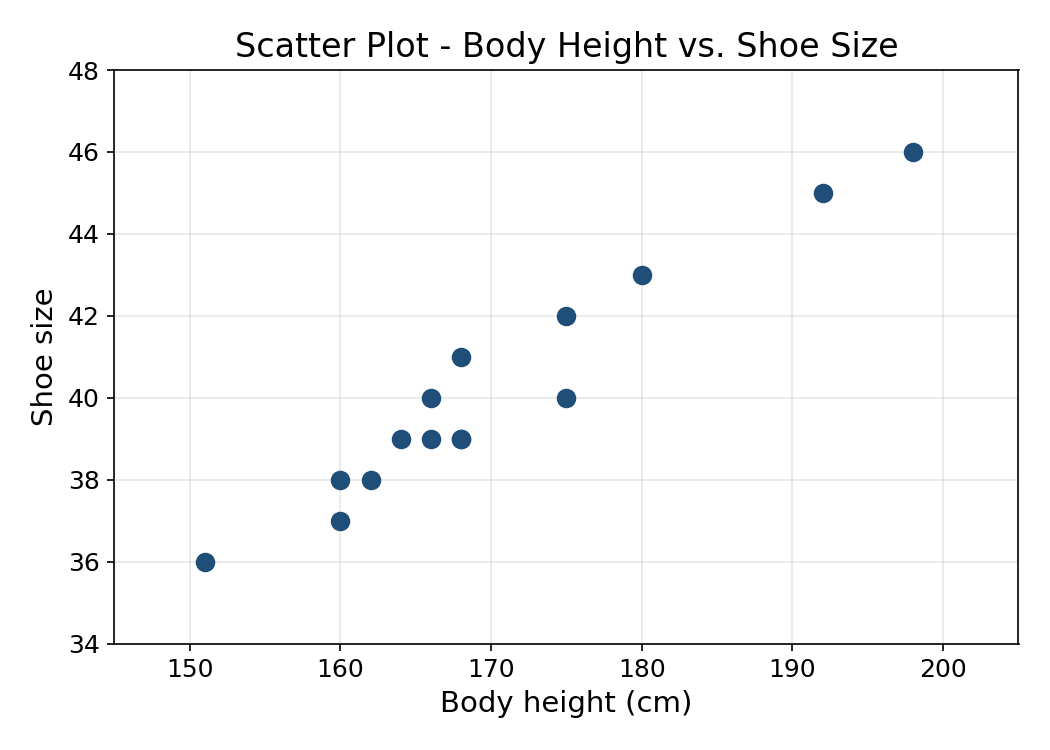
\includegraphics[width=\textwidth,height=0.72\textheight,keepaspectratio]{images/image_026_en.png}
    \end{column}
    \begin{column}{0.5\textwidth}
      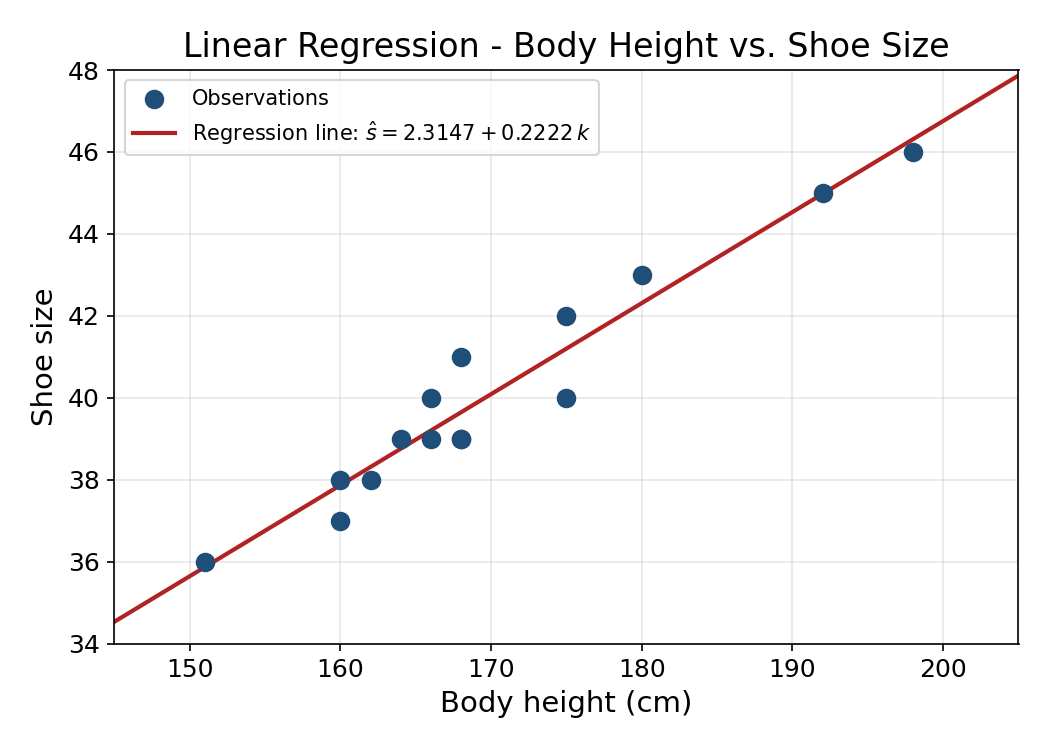
\includegraphics[width=\textwidth,height=0.72\textheight,keepaspectratio]{images/image_027_en.png}
    \end{column}
  \end{columns}
\end{frame}

\begin{frame}{Solution Task 2 -- residual plot}
  \begin{columns}[c]
    \begin{column}{0.62\textwidth}
      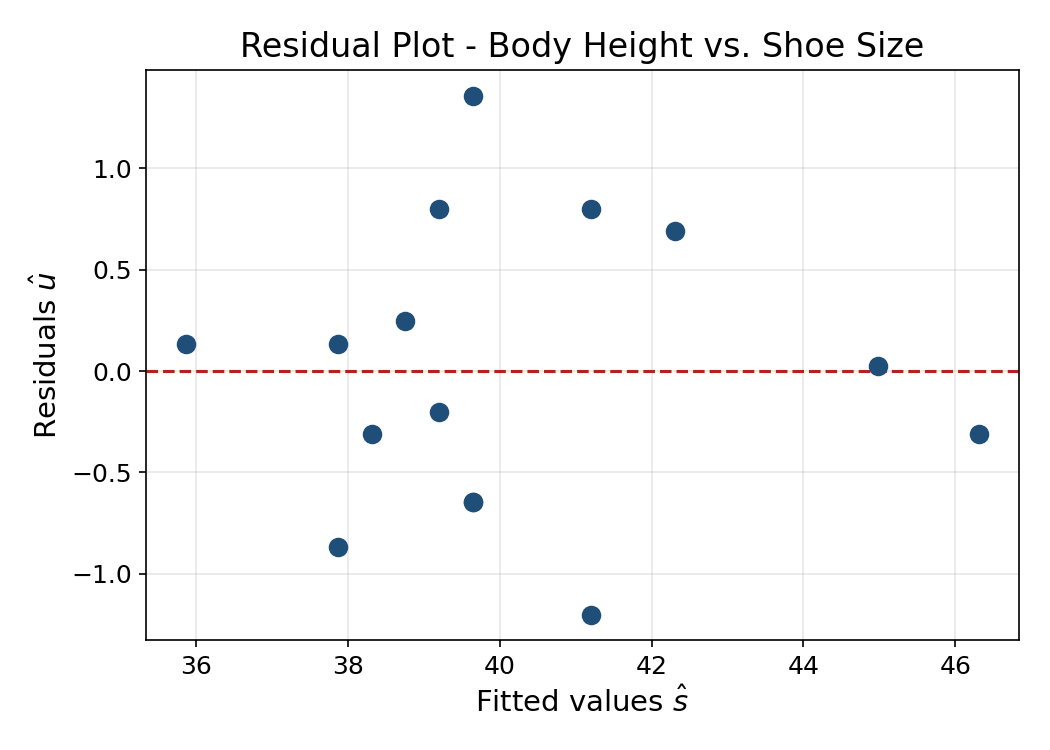
\includegraphics[width=\textwidth,height=0.76\textheight,keepaspectratio]{images/image_028_en.png}
    \end{column}
    \begin{column}{0.35\textwidth}
      \begin{exampleblock}{Observation}
        \textbf{No systematic structure visible} \checkmark\ -- no curve,
        no funnel.
      \end{exampleblock}
    \end{column}
  \end{columns}
\end{frame}

\begin{frame}{Solution Task 3 -- QQ-plot of the residuals}
  \begin{columns}[c]
    \begin{column}{0.56\textwidth}
      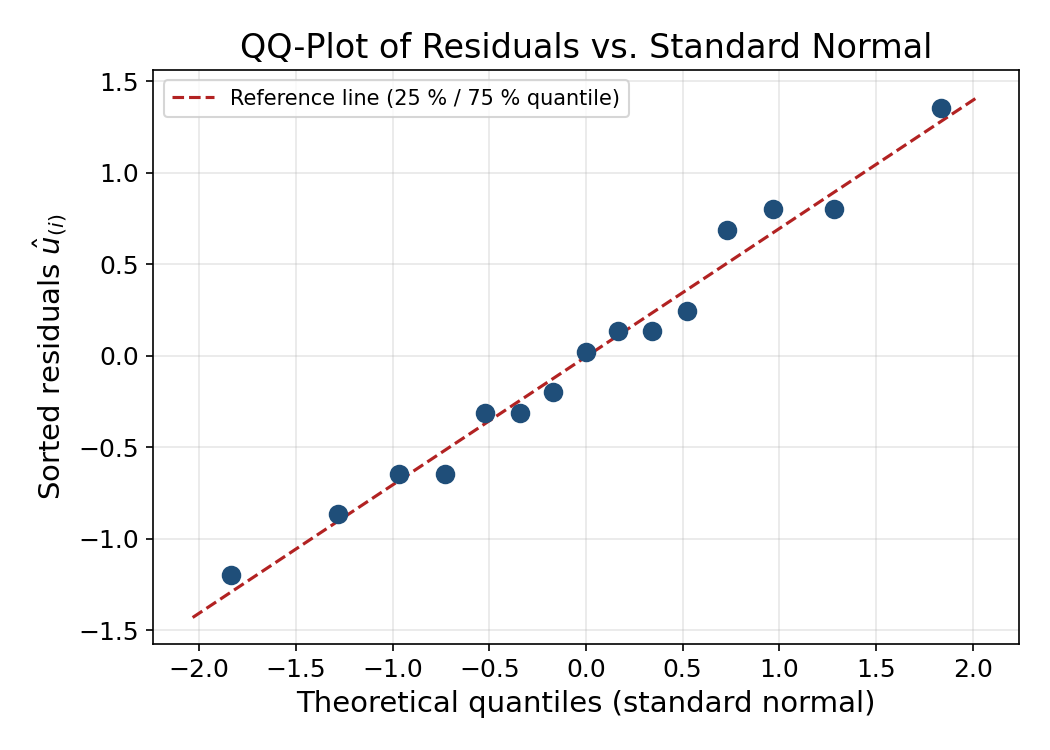
\includegraphics[width=\textwidth,height=0.7\textheight,keepaspectratio]{images/image_029_en.png}
    \end{column}
    \begin{column}{0.42\textwidth}
      \footnotesize
      \textbf{Procedure:} residuals $\hat u_i=s_i-\hat s_i$, sorted;
      normal quantiles $z_i=\Phi^{-1}\bigl(\tfrac{i-0.5}{15}\bigr)$; plot
      $(z_i,\hat u_{(i)})$.
      \begin{exampleblock}{Conclusion}
        The points lie almost perfectly on the line --
        \textbf{the normality assumption is met}. This model is a good
        candidate for inference (next section).
      \end{exampleblock}
    \end{column}
  \end{columns}
\end{frame}

% ============================================================================
% SECTION 5: INFERENCE IN SIMPLE REGRESSION
% ============================================================================
\section[Inference]{Inference in Simple Regression}

\subsection{Sampling variability}

\begin{frame}{Why regression coefficients carry uncertainty}
  \begin{block}{Intuition (as in Part~3)}
    The nine stores are only a \textbf{sample}. Other stores -- or the same
    stores in another week -- would give slightly different sales, hence a
    slightly different line.
  \end{block}
  \begin{itemize}\setlength{\itemsep}{3pt}
    \item The \textbf{true} coefficients $\beta_0,\beta_1$ (population line)
          are fixed but unknown.
    \item The \textbf{estimates} $\hat\beta_0,\hat\beta_1$ are computed from
          a random sample -- they are \textbf{random variables} with a
          sampling distribution, exactly like $\bar X$ in Part~3.
    \item Questions: How much does $\hat\beta_1$ wobble? Is the true slope
          possibly $0$? Which values of $\beta_1$ are compatible with the
          data?
  \end{itemize}
  \kernaussage{The tools are the same as for the mean: \textbf{standard
  error}, \textbf{$t$-test}, \textbf{confidence interval} and
  \textbf{$p$-value}.}
\end{frame}

\begin{frame}{Population line vs.\ sample lines}
  \begin{center}
    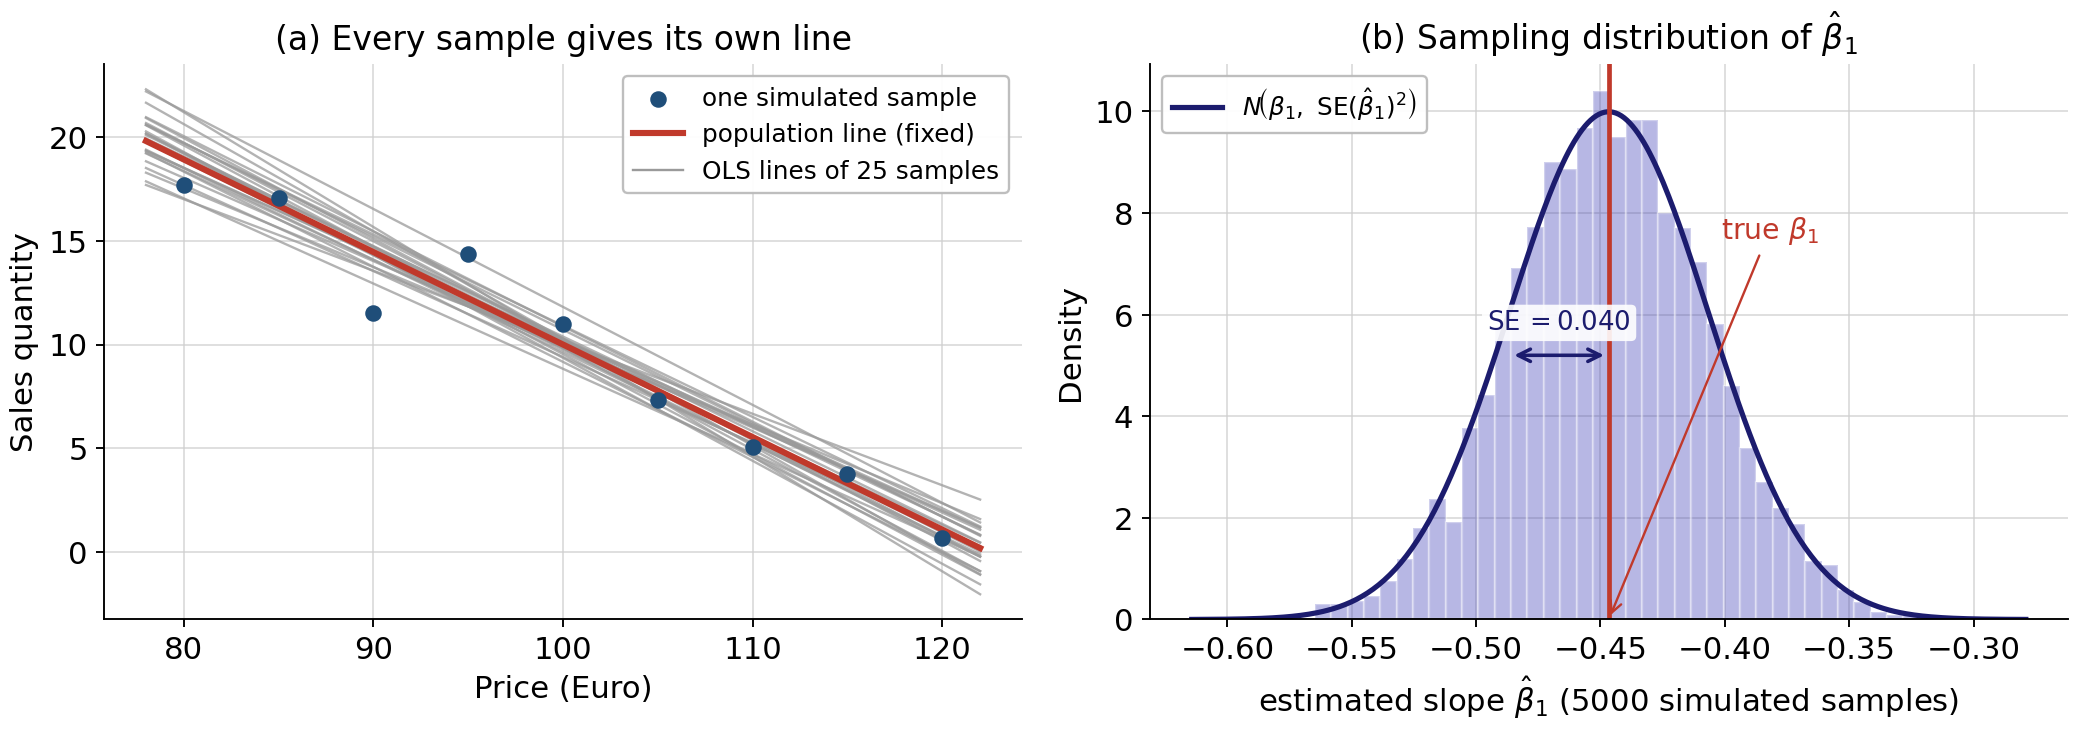
\includegraphics[width=0.97\textwidth,height=0.62\textheight,keepaspectratio]{images/reg_sampling_lines.png}
  \end{center}
  \footnotesize Simulation with the lamp prices: (a) every sample gives its
  own OLS line around the fixed population line; (b) over $5000$ samples the
  slopes $\hat\beta_1$ are normally distributed around $\beta_1$ -- their
  standard deviation is the \textbf{standard error}.
\end{frame}

\begin{frame}{Sampling distribution of the slope}
  \begin{block}{Result (under the four assumptions on $u_i$)}
    \[
      \hat\beta_1 \sim N\!\left(\beta_1,\ \frac{\sigma^2}{S_{xx}}\right),
      \qquad
      \mathrm{SE}(\hat\beta_1)=\frac{\sigma}{\sqrt{S_{xx}}}
      =\frac{\sigma}{\sqrt{\sum_i (x_i-\bar x)^2}} .
    \]
  \end{block}
  \begin{itemize}\setlength{\itemsep}{3pt}
    \item $E(\hat\beta_1)=\beta_1$: the estimator is \textbf{unbiased} --
          on average it hits the true slope.
    \item \textbf{Less noise} ($\sigma\downarrow$) $\Rightarrow$ smaller SE.
    \item \textbf{More spread in $x$} ($S_{xx}\uparrow$) $\Rightarrow$ smaller
          SE: a long ``lever arm'' fixes the slope precisely.
    \item \textbf{More observations} increase $S_{xx}$ $\Rightarrow$
          smaller SE.
  \end{itemize}
  \inworten{Compare Part~3: $\mathrm{SE}(\bar X)=\sigma/\sqrt n$. Here the
  role of $n$ is taken by $S_{xx}$.}
\end{frame}

\begin{frame}{Estimating $\sigma$: the residual standard error}
  \begin{block}{Problem}
    The error variance $\sigma^2$ is unknown -- as $\sigma$ in Part~3. We
    estimate it from the residuals.
  \end{block}
  \begin{block}{Residual standard error}
    \[
      \hat\sigma=\sqrt{\frac{\text{RSS}}{n-2}}
      =\sqrt{\frac{1}{n-2}\sum_{i=1}^n \hat u_i^{\,2}},
      \qquad
      \mathrm{SE}(\hat\beta_1)=\frac{\hat\sigma}{\sqrt{S_{xx}}},
      \qquad
      \mathrm{SE}(\hat\beta_0)=\hat\sigma\sqrt{\frac1n+\frac{\bar x^2}{S_{xx}}} .
    \]
  \end{block}
  \begin{itemize}
    \item \textbf{Why $n-2$?} Two parameters ($\beta_0,\beta_1$) were
          estimated -- two degrees of freedom are used up (Part~1: one
          parameter $\bar x$ $\Rightarrow$ $n-1$).
    \item $\hat\sigma$ is measured in the \textbf{units of $y$}: the typical
          size of a residual.
  \end{itemize}
\end{frame}

\begin{frame}{Standard errors -- lamp example}
  \textbf{Given:} $n=9$, $\text{RSS}=16.733$, $S_{xx}=1500$, $\bar x=100$.
  \begin{exampleblock}{Calculation}
    \begin{align*}
      \hat\sigma &= \sqrt{\frac{16.733}{9-2}}=\sqrt{2.3905}=\mathbf{1.5461}\\[3pt]
      \mathrm{SE}(\hat\beta_1) &= \frac{1.5461}{\sqrt{1500}}=\frac{1.5461}{38.730}=\mathbf{0.03992}\\[3pt]
      \mathrm{SE}(\hat\beta_0) &= 1.5461\sqrt{\frac19+\frac{100^2}{1500}}
                    =1.5461\cdot 2.6034=\mathbf{4.0252}
    \end{align*}
  \end{exampleblock}
  \inworten{A typical store deviates by about $1.5$ lamps from the line; the
  slope $-0.4467$ is uncertain by about $\pm 0.04$ (one standard error).}
\end{frame}

\subsection{$t$-test for a coefficient}

\begin{frame}{The first question: is there any relationship at all?}
  \begin{block}{Hypotheses}
    \[
      H_0: \beta_1 = 0 \qquad\text{vs.}\qquad H_1: \beta_1 \ne 0
    \]
  \end{block}
  \begin{itemize}\setlength{\itemsep}{3pt}
    \item $H_0$: the price has \textbf{no} (linear) influence on the sales
          quantity -- the population line is flat.
    \item $H_1$: the price has \emph{some} influence.
    \item As in Part~3: what we want to \textbf{establish} goes into $H_1$.
  \end{itemize}
  \kernaussage{Rejecting $H_0:\beta_1=0$ is what licenses us to interpret the
  slope at all -- a slope that could just as well be zero tells us nothing.}
\end{frame}

\begin{frame}{The $t$-statistic -- the same recipe as in Part~3}
  \begin{block}{Test statistic}
    \[
      T=\frac{\hat\beta_1-\beta_{1,0}}{\mathrm{SE}(\hat\beta_1)}
      \;\sim\; t_{n-2}\ \text{ under } H_0:\beta_1=\beta_{1,0}
      \qquad(\text{usually } \beta_{1,0}=0)
    \]
  \end{block}
  \begin{center}
    \renewcommand{\arraystretch}{1.3}
    \begin{tabular}{lcc}
      \toprule
      & \textbf{Part 3: mean} & \textbf{Part 4: slope}\\
      \midrule
      Estimate & $\bar x$ & $\hat\beta_1$\\
      Hypothesized value & $\mu_0$ & $\beta_{1,0}$ (mostly $0$)\\
      Standard error & $s/\sqrt n$ & $\hat\sigma/\sqrt{S_{xx}}$\\
      Distribution under $H_0$ & $t_{n-1}$ & $t_{n-2}$\\
      Reject (two-sided) if & $|T_n|>t_{1-\alpha/2,\,n-1}$ & $|T|>t_{1-\alpha/2,\,n-2}$\\
      \bottomrule
    \end{tabular}
  \end{center}
  \inworten{``How many standard errors is the estimate away from the
  hypothesized value?''}
\end{frame}

\begin{frame}{The test recipe for a regression coefficient}
  \centering
  \resizebox{\textwidth}{!}{%
  \begin{tikzpicture}[node distance=6mm]
    \node[flowbox, text width=2.5cm] (h)
      {\footnotesize \textbf{1. Hypotheses}\\ $H_0:\beta_1=0$\\ $H_1:\beta_1\neq0$};
    \node[flowbox, text width=2.9cm, right=8mm of h] (z)
      {\footnotesize \textbf{2. Test statistic}\\ $T=\dfrac{\hat\beta_1}{\mathrm{SE}(\hat\beta_1)}$};
    \node[flowbox, text width=2.5cm, right=8mm of z] (c)
      {\footnotesize \textbf{3. crit.\ value}\\ $t_{1-\alpha/2,\,n-2}$};
    \node[diamond, draw=hsbiblaudunkel, very thick, fill=hsbiblau!8,
          aspect=2, inner sep=1pt, text width=2.3cm, align=center,
          right=8mm of c] (d) {\scriptsize $|T|>t_{1-\alpha/2,n-2}$?};
    \node[flowboxo, text width=2.3cm, above right=2mm and 8mm of d] (ja)
      {\footnotesize \textbf{yes:} reject $H_0$};
    \node[flowboxg, text width=2.3cm, below right=2mm and 8mm of d] (nein)
      {\footnotesize \textbf{no:} keep $H_0$};
    \draw[flowarr] (h)--(z); \draw[flowarr] (z)--(c); \draw[flowarr] (c)--(d);
    \draw[flowarr] (d.north) to[out=90,in=180] (ja.west);
    \draw[flowarr] (d.south) to[out=-90,in=180] (nein.west);
  \end{tikzpicture}}
  \vspace{0.8em}
  \begin{itemize}
    \item Fix $\alpha$ (typically $0.05$) \emph{before} looking at the data.
    \item Equivalent decision via the $p$-value: reject $H_0$ if
          $p<\alpha$, with $p=2\,F_{t,n-2}(-|T|)$.
  \end{itemize}
\end{frame}

\begin{frame}{$t$-test -- lamp example}
  \textbf{Data:} $\hat\beta_1=-0.4467$, $\mathrm{SE}(\hat\beta_1)=0.03992$,
  $n=9$, $\alpha=0.05$, $t_{0.975;\,7}=2.3646$.
  \begin{align*}
    T &= \frac{-0.4467-0}{0.03992} = -11.19\\[2pt]
    |T| &= 11.19 \;>\; 2.3646 = t_{0.975;\,7}
  \end{align*}
  \begin{alertblock}{Decision}
    $H_0:\beta_1=0$ is \textbf{rejected}. The price has a significant
    influence on the sales quantity. The $p$-value is
    $p=2\,F_{t,7}(-11.19)=0.00001$.
  \end{alertblock}
  \inworten{The estimated slope lies more than eleven standard errors away
  from zero -- far too far to be a chance result.}
\end{frame}

\begin{frame}{Testing other hypothesized values}
  \textbf{Question:} A marketing study claims that each Euro of price costs
  \emph{half} a lamp. Is this compatible with our data?
  \[
    H_0:\beta_1=-0.5 \quad\text{vs.}\quad H_1:\beta_1\neq-0.5
  \]
  \begin{exampleblock}{Test}
    \[
      T=\frac{-0.4467-(-0.5)}{0.03992}=\frac{0.0533}{0.03992}=1.336,
      \qquad |T|=1.336<2.3646=t_{0.975;\,7}
    \]
    $\Rightarrow$ \textbf{keep} $H_0$ \ ($p=0.223$).
  \end{exampleblock}
  \begin{block}{Reading}
    The data cannot distinguish $\beta_1=-0.5$ from the estimate $-0.4467$:
    the claim is \emph{compatible} with the data -- but not \emph{proven}.
  \end{block}
\end{frame}

\begin{frame}{Two $t$-tests in one picture}
  \begin{center}
    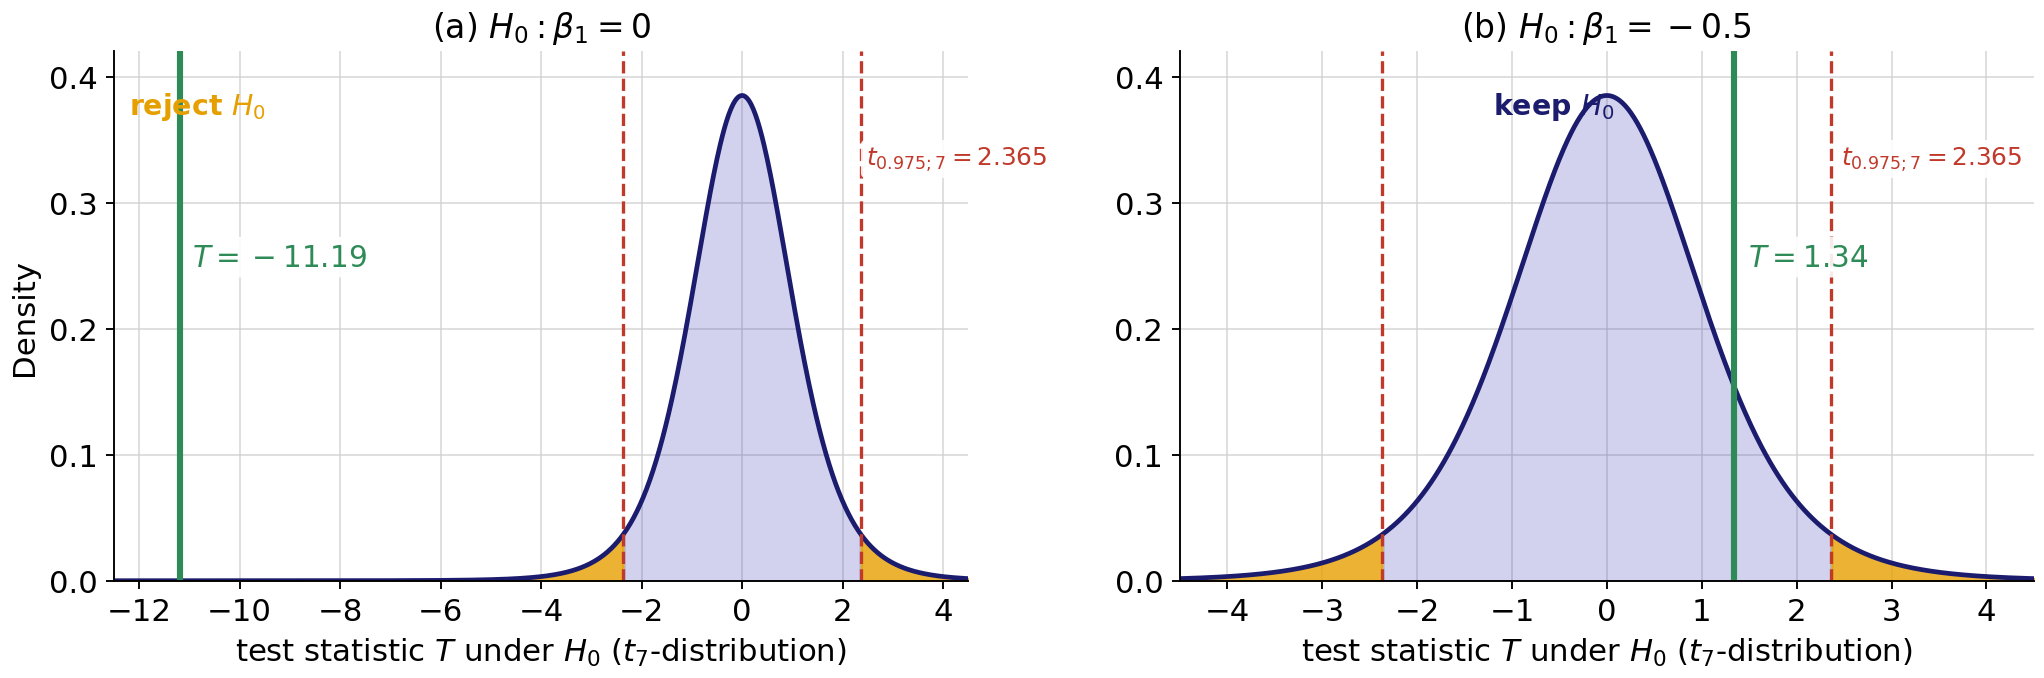
\includegraphics[width=0.97\textwidth,height=0.6\textheight,keepaspectratio]{images/reg_slope_tests.png}
  \end{center}
  \footnotesize Both tests use the same $t_7$-distribution and the same bars
  $\pm2.365$. (a) $T=-11.19$ lies far in the rejection region (orange);
  (b) $T=1.34$ lies inside the acceptance region. The decision is nothing more
  than: \textbf{where does the statistic fall?}
\end{frame}

\begin{frame}{One-sided test for the slope}
  \begin{block}{Economic theory gives a direction}
    A price-sales function should \emph{fall}. We want evidence for a
    negative slope:
    \[
      H_0:\beta_1=0 \quad\text{vs.}\quad H_1:\beta_1<0 \qquad(\text{left-sided})
    \]
  \end{block}
  \begin{exampleblock}{Lamp example}
    Reject if $T<-t_{1-\alpha,\,n-2}=-t_{0.95;\,7}=-1.8946$:
    \[
      T=-11.19<-1.8946\ \Rightarrow\ \text{reject }H_0,
      \qquad p=F_{t,7}(-11.19)=0.000005 .
    \]
  \end{exampleblock}
  \begin{alertblock}{As in Part~3}
    The direction must be fixed \emph{before} looking at the data, and the
    one-sided $p$-value is half the two-sided one only if $T$ points in the
    direction of $H_1$. \texttt{R} always reports the \textbf{two-sided}
    $p$-value.
  \end{alertblock}
\end{frame}

\begin{frame}{Before you test -- the assumptions checklist}
  \begin{enumerate}\setlength{\itemsep}{5pt}
    \item \textbf{Linear model is correct} -- residual plot without
          systematic pattern.
    \item \textbf{Independent observations} -- no autocorrelation (e.g.\
          not the same store measured repeatedly).
    \item \textbf{Constant variance} -- no funnel in the residual plot.
    \item \textbf{Normally distributed errors} -- QQ-plot; for large $n$ the
          central limit theorem makes the $t$-test approximately valid
          anyway.
  \end{enumerate}
  \kernaussage{If the assumptions fail, the standard errors -- and with them
  every $t$-test, confidence interval and $p$-value -- are not reliable. The
  point estimates $\hat\beta_0,\hat\beta_1$ may still be fine.}
\end{frame}

\subsection{Confidence intervals}

\begin{frame}{Confidence interval for $\beta_1$}
  \begin{block}{Construction -- exactly as for $\mu$ in Part~3}
    \[
      \text{CI}_{1-\alpha}(\beta_1)
      =\Bigl[\hat\beta_1-t_{1-\alpha/2,\,n-2}\,\mathrm{SE}(\hat\beta_1),\;
             \hat\beta_1+t_{1-\alpha/2,\,n-2}\,\mathrm{SE}(\hat\beta_1)\Bigr]
    \]
  \end{block}
  \[
    \text{CI} = \big[\;\underbrace{\hat\beta_1}_{\text{estimate}}
       \;\pm\; \underbrace{t_{1-\alpha/2,\,n-2}}_{\substack{\text{critical}\\\text{value}}}
       \cdot \underbrace{\mathrm{SE}(\hat\beta_1)}_{\text{standard error}}\;\big]
  \]
  \inworten{For large $n$ the critical value is close to $1.96\approx2$:
  $\hat\beta_1\pm2\,\mathrm{SE}(\hat\beta_1)$ is a quick $95\,\%$ interval.}
\end{frame}

\begin{frame}{Confidence interval -- lamp example}
  \textbf{Given:} $\hat\beta_1=-0.4467$, $\mathrm{SE}(\hat\beta_1)=0.03992$,
  $t_{0.975;\,7}=2.3646$.
  \begin{align*}
    \text{margin of error } e &= 2.3646\cdot 0.03992 = 0.0944\\
    \text{CI}_{0.95}(\beta_1) &= [\,-0.4467\pm0.0944\,]
      = \mathbf{[\,-0.5411\,;\,-0.3523\,]}
  \end{align*}
  \begin{exampleblock}{Interpretation}
    The procedure covers the true slope in $95\,\%$ of all samples. Values
    of $\beta_1$ between $-0.54$ and $-0.35$ lamps per Euro are
    \emph{compatible} with the data.
  \end{exampleblock}
  \begin{block}{Duality with the test}
    $0\notin\text{CI}$ $\Leftrightarrow$ $H_0:\beta_1=0$ is rejected;
    \quad $-0.5\in\text{CI}$ $\Leftrightarrow$ $H_0:\beta_1=-0.5$ is kept.
  \end{block}
\end{frame}

\begin{frame}{Confidence intervals -- interpretation pitfalls}
  \begin{alertblock}{Careful with the interpretation}
    ``With $95\,\%$ probability $\beta_1$ lies in \emph{this particular}
    interval $[-0.5411;\,-0.3523]$'' is, strictly speaking, \textbf{wrong}.
  \end{alertblock}
  \begin{itemize}\setlength{\itemsep}{3pt}
    \item $\beta_1$ is a fixed (unknown) number; the \emph{bounds} of the
          interval are random.
    \item Correct: ``The \textbf{procedure} yields, in $95\,\%$ of samples,
          an interval that covers $\beta_1$.''
  \end{itemize}
  \begin{block}{Intercept}
    The CI for $\beta_0$ is $[45.15;\,64.18]$. It is computed in the same
    way -- but $\beta_0$ (sales at price $0$) has no substantive meaning
    here.
  \end{block}
\end{frame}

\subsection{$p$-values and R output}

\begin{frame}{The $p$-value of a coefficient}
  \begin{block}{Definition (as in Part~3)}
    The $p$-value is the probability, under $H_0:\beta_1=0$, of a test
    statistic that is \textbf{at least as extreme} as the observed one:
    \[
      p=P\bigl(|T|\ge|T_{\text{obs}}|\,\big|\,H_0\bigr)=2\,F_{t,n-2}\bigl(-|T_{\text{obs}}|\bigr).
    \]
  \end{block}
  \begin{center}
    \renewcommand{\arraystretch}{1.25}
    \begin{tabular}{lccc}
      \toprule
      Hypothesis (lamp) & $T$ & $p$ (two-sided) & Decision at $\alpha=0.05$\\
      \midrule
      $H_0:\beta_1=0$ & $-11.19$ & $0.00001$ & reject\\
      $H_0:\beta_1=-0.5$ & $1.34$ & $0.223$ & keep\\
      \bottomrule
    \end{tabular}
  \end{center}
  \kernaussage{$p<\alpha$ $\Leftrightarrow$ $|T|>t_{1-\alpha/2,\,n-2}$
  $\Leftrightarrow$ hypothesized value outside the CI.}
\end{frame}

\begin{frame}[fragile]{Reading the regression output in R}
\begin{lstlisting}[style=Rout]
> summary(lm(quantity ~ price))
Coefficients:
            Estimate Std. Error t value Pr(>|t|)
(Intercept) 54.66667    4.02519   13.58 2.76e-06 ***
price       -0.44667    0.03992  -11.19 1.02e-05 ***
---
Residual standard error: 1.546 on 7 degrees of freedom
Multiple R-squared:  0.947,  Adjusted R-squared:  0.9395
F-statistic: 125.2 on 1 and 7 DF,  p-value: 1.016e-05
\end{lstlisting}
  \begin{center}
    \footnotesize
    \renewcommand{\arraystretch}{1.1}
    \begin{tabular}{@{}ll@{}}
      \toprule
      \texttt{Estimate}, \texttt{Std. Error} & $\hat\beta_j$ and $\mathrm{SE}(\hat\beta_j)$\\
      \texttt{t value}, \texttt{Pr(>|t|)} & $T$ for $H_0:\beta_j=0$ and its two-sided $p$-value\\
      \texttt{Residual standard error} & $\hat\sigma=\sqrt{\text{RSS}/(n-2)}$ with $n-2=7$ degrees of freedom\\
      \texttt{Multiple R-squared} & $R^2$ \quad (adjusted $R^2$: see multiple regression)\\
      \texttt{F-statistic} & tests all slopes jointly; here $F=T^2=(-11.19)^2=125.2$\\
      \bottomrule
    \end{tabular}
  \end{center}
\end{frame}

\begin{frame}{Significant $\neq$ important}
  \begin{block}{The $p$-value measures evidence, not size}
    With many observations even a tiny slope becomes highly significant. The
    size of the effect is read from $\hat\beta_1$ and its confidence
    interval.
  \end{block}
  \begin{exampleblock}{Advertising data ($n=200$): sales on TV budget}
    $\hat\beta_1=0.0475$ (sales in $1000$ units, budget in $1000$\,\$),
    $\mathrm{SE}=0.0027$, $T=17.67$, $p<0.0001$,
    $\text{CI}_{0.95}=[0.0422;\,0.0528]$.
    \begin{itemize}
      \item \emph{Significance:} overwhelming evidence that TV advertising
            and sales are related.
      \item \emph{Size:} $1000$\,\$ more TV budget goes along with
            $42$ to $53$ additional units sold -- whether this pays off is
            a business question, not a statistical one.
    \end{itemize}
  \end{exampleblock}
  \kernaussage{Report the estimate \emph{and} its confidence interval -- not
  just the $p$-value or the stars.}
\end{frame}

\subsection{Prediction}

\begin{frame}{Two questions about a new $x_0$}
  At a new price $x_0$ the prediction is $\hat y_0=\hat\beta_0+\hat\beta_1x_0$.
  How precise is it? It depends on the question:
  \begin{columns}[T]
    \begin{column}{0.48\textwidth}
      \begin{block}{Confidence interval}
        for the \textbf{mean} sales $E(Y\mid x_0)$ of \emph{all} stores
        with price $x_0$:
        \[
          \hat y_0\pm t_{1-\alpha/2,\,n-2}\,\hat\sigma
          \sqrt{\frac1n+\frac{(x_0-\bar x)^2}{S_{xx}}}
        \]
      \end{block}
    \end{column}
    \begin{column}{0.48\textwidth}
      \begin{block}{Prediction interval}
        for the sales $Y_0$ of \textbf{one} new store with price $x_0$:
        \[
          \hat y_0\pm t_{1-\alpha/2,\,n-2}\,\hat\sigma
          \sqrt{1+\frac1n+\frac{(x_0-\bar x)^2}{S_{xx}}}
        \]
      \end{block}
    \end{column}
  \end{columns}
  \kernaussage{The ``$1+$'' adds the error $u_0$ of the single store: a
  prediction interval is \textbf{always wider} and never shrinks below
  $\pm t\,\hat\sigma$, however large $n$ becomes.}
\end{frame}

\begin{frame}{Prediction -- lamp example}
  \textbf{Given:} $\hat\sigma=1.5461$, $n=9$, $\bar x=100$, $S_{xx}=1500$,
  $t_{0.975;\,7}=2.3646$, new price $x_0=110$:
  $\hat y_0=54.67-0.4467\cdot110=5.53$.
  \begin{exampleblock}{Calculation}
    \begin{align*}
      \text{CI: }& 5.53\pm2.3646\cdot1.5461\sqrt{\tfrac19+\tfrac{100}{1500}}
        =5.53\pm1.54=[\,3.99\,;\,7.07\,]\\[2pt]
      \text{PI: }& 5.53\pm2.3646\cdot1.5461\sqrt{1+\tfrac19+\tfrac{100}{1500}}
        =5.53\pm3.97=[\,1.57\,;\,9.50\,]
    \end{align*}
  \end{exampleblock}
  \begin{block}{Reading}
    At $110$ Euro, stores sell on \emph{average} between $4$ and $7$ lamps
    ($95\,\%$ CI); a \emph{single} new store will sell between about $2$ and
    $9$ lamps ($95\,\%$ PI).
  \end{block}
\end{frame}

\begin{frame}{Confidence band vs.\ prediction band}
  \begin{columns}[c]
    \begin{column}{0.64\textwidth}
      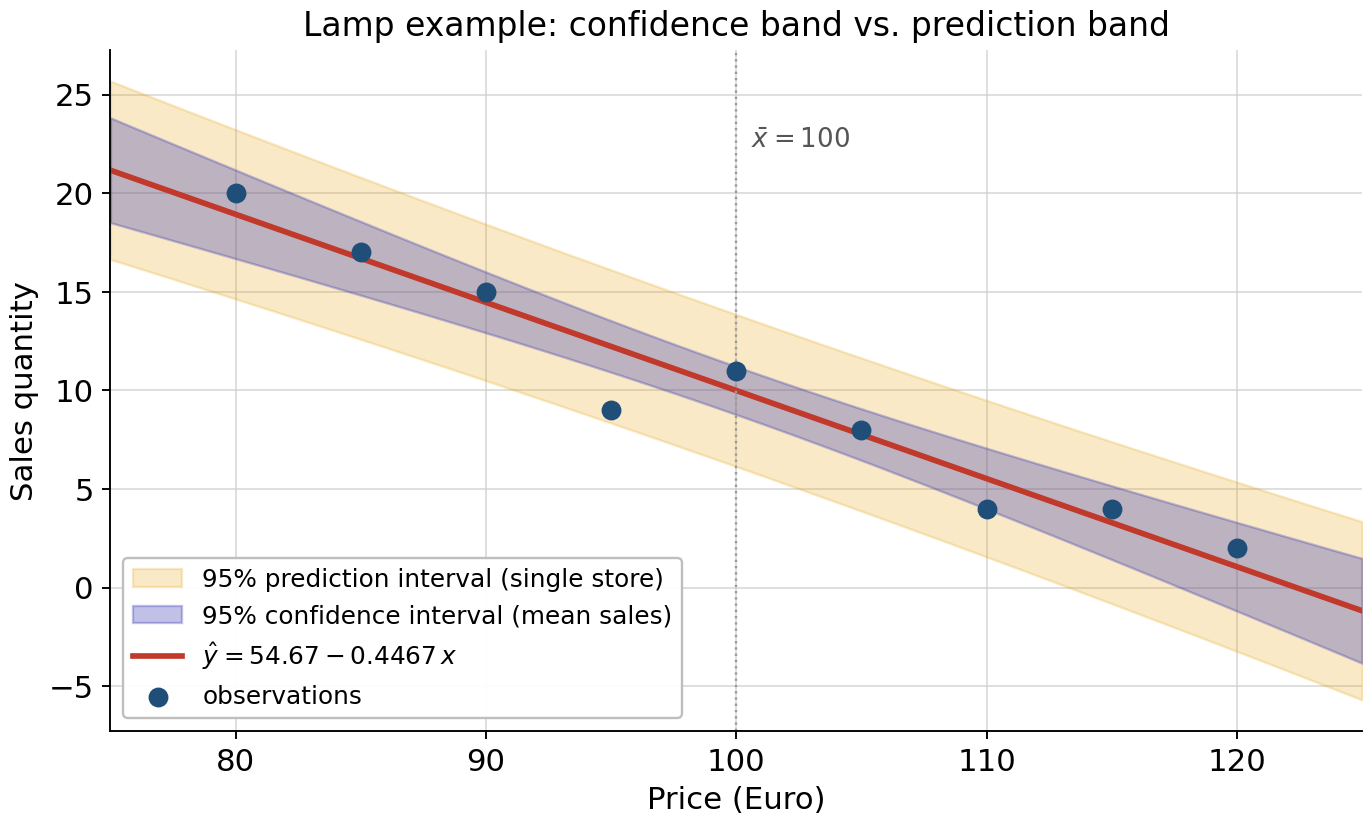
\includegraphics[width=\textwidth,height=0.74\textheight,keepaspectratio]{images/reg_lamp_ci_pi.png}
    \end{column}
    \begin{column}{0.34\textwidth}
      \footnotesize
      \begin{itemize}\setlength{\itemsep}{4pt}
        \item Both bands are narrowest at $\bar x=100$ and widen towards the
              edges.
        \item The prediction band contains most of the points; the
              confidence band does not need to.
      \end{itemize}
      \begin{alertblock}{Extrapolation}
        At $x_0=125$ Euro the line predicts $\hat y_0=-1.17$ lamps --
        impossible. Outside the data range the linear model breaks down.
      \end{alertblock}
    \end{column}
  \end{columns}
\end{frame}

\begin{frame}[fragile]{Inference in simple regression with R (1/2)}
  \begin{block}{Tests, $p$-values and confidence intervals}
\begin{lstlisting}
reg <- lm(quantity ~ price)
summary(reg)                     # estimates, SE, t, p, R^2
confint(reg, level = 0.95)       # CI for beta0 and beta1
\end{lstlisting}
  \end{block}
  \begin{block}{By hand}
\begin{lstlisting}
se_b1 <- summary(reg)$coefficients["price", "Std. Error"]
T <- (coef(reg)["price"] - (-0.5)) / se_b1    # H0: beta1 = -0.5
2 * pt(-abs(T), df = 7)                       # p-value 0.223
qt(0.975, df = 7)                             # critical value 2.3646
\end{lstlisting}
  \end{block}
\end{frame}

\begin{frame}[fragile]{Inference in simple regression with R (2/2)}
  \begin{block}{Prediction}
\begin{lstlisting}
new <- data.frame(price = 110)
predict(reg, new, interval = "confidence")    # mean sales: [3.99, 7.07]
predict(reg, new, interval = "prediction")    # one store:  [1.57, 9.50]
\end{lstlisting}
  \end{block}
  \begin{exampleblock}{Note}
    \texttt{predict()} needs a data frame whose column has \emph{the same
    name} as the explanatory variable in the model (here \texttt{price}).
  \end{exampleblock}
\end{frame}

\subsection{Exercises}

\begin{frame}{Exercise -- standard error, $t$ and confidence interval}
  \begin{block}{Problem statement}
    A simple linear regression on $n=10$ observations gives
    $\hat\beta_1 = 2.5$, residual standard error $\hat\sigma=4.0$ and
    $S_{xx}=\sum(x_i-\bar x)^2 = 16$.
    \begin{enumerate}
      \item Compute the standard error $\mathrm{SE}(\hat\beta_1)$.
      \item Compute the $t$-statistic for $H_0:\beta_1=0$.
      \item Compute the $95\,\%$ confidence interval for $\beta_1$.
      \item Is the slope significant at the $5\,\%$ level? Justify in two
            ways.
    \end{enumerate}
  \end{block}
  \textbf{Hint:} $t_{0.975;\,8}=2.306$.
\end{frame}

\begin{frame}{Solution -- standard error, $t$ and confidence interval}
  \begin{align*}
    \textbf{(1)}\quad \mathrm{SE}(\hat\beta_1)&=\frac{\hat\sigma}{\sqrt{S_{xx}}}
      =\frac{4.0}{\sqrt{16}}=\mathbf{1.0}\\[2pt]
    \textbf{(2)}\quad T&=\frac{2.5-0}{1.0}=\mathbf{2.5},\qquad \text{df}=n-2=8\\[2pt]
    \textbf{(3)}\quad \text{CI}_{0.95}&=2.5\pm2.306\cdot1.0=\mathbf{[\,0.194\,;\,4.806\,]}
  \end{align*}
  \begin{exampleblock}{(4) Decision}
    $|T|=2.5>2.306$ -- equivalently, $0$ lies outside the CI. $H_0:\beta_1=0$
    is rejected at $\alpha=0.05$ ($p\approx0.037$).
  \end{exampleblock}
  \inworten{Common mistake: dividing $\hat\sigma$ by $\sqrt n$ -- the standard
  error of the slope divides by $\sqrt{S_{xx}}$.}
\end{frame}

\begin{frame}{Exercise -- inference for the shoe-size regression}
  \begin{block}{Problem statement}
    For the body heights and shoe sizes ($n=15$) we found
    $\hat s=2.3147+0.2222\,k$. In addition: $\text{RSS}=6.9432$,
    $S_{kk}=2122.4$, $\bar k=170.2$.
    \begin{enumerate}
      \item Compute $\hat\sigma$ and $\mathrm{SE}(\hat\beta_1)$.
      \item Test $H_0:\beta_1=0$ at $\alpha=0.05$.
      \item Compute the $95\,\%$ confidence interval for $\beta_1$.
      \item A rule of thumb says ``one shoe size per $4\,$cm'', i.e.\
            $\beta_1=0.25$. Test this claim.
      \item Give a $95\,\%$ prediction interval for the shoe size of a
            person with $k_0=180\,$cm.
    \end{enumerate}
  \end{block}
  \textbf{Hint:} $t_{0.975;\,13}=2.1604$.
\end{frame}

\begin{frame}{Solution (1/3) -- inference for the shoe-size regression}
  \begin{exampleblock}{(1) Residual standard error and standard error}
    \[
      \hat\sigma=\sqrt{\frac{6.9432}{15-2}}=\sqrt{0.5341}=0.7308,
      \qquad
      \mathrm{SE}(\hat\beta_1)=\frac{0.7308}{\sqrt{2122.4}}=\frac{0.7308}{46.069}=0.01586
    \]
  \end{exampleblock}
  \begin{exampleblock}{(2) $t$-test for $H_0:\beta_1=0$}
    \[
      T=\frac{0.2222}{0.01586}=14.01\;>\;2.1604=t_{0.975;\,13}
      \quad\Rightarrow\quad \text{reject } H_0 \quad (p=3.2\cdot10^{-9}).
    \]
  \end{exampleblock}
  \inworten{Body height is a highly significant predictor of shoe size.}
\end{frame}

\begin{frame}{Solution (2/3) -- inference for the shoe-size regression}
  \begin{exampleblock}{(3) Confidence interval}
    \[
      0.2222\pm2.1604\cdot0.01586=0.2222\pm0.0343=\mathbf{[\,0.1879\,;\,0.2565\,]}
    \]
    Between $0.19$ and $0.26$ shoe sizes per cm are compatible with the data.
  \end{exampleblock}
  \begin{exampleblock}{(4) $H_0:\beta_1=0.25$}
    \[
      T=\frac{0.2222-0.25}{0.01586}=-1.75,\qquad |T|=1.75<2.1604
      \quad\Rightarrow\quad\text{keep } H_0\ (p=0.103).
    \]
    Consistent with the CI: $0.25\in[0.1879;\,0.2565]$.
  \end{exampleblock}
  \begin{alertblock}{Careful}
    ``Keep $H_0$'' does not prove the rule of thumb -- the data are merely
    \emph{compatible} with it.
  \end{alertblock}
\end{frame}

\begin{frame}{Solution (3/3) -- inference for the shoe-size regression}
  \begin{exampleblock}{(5) Prediction interval at $k_0=180$}
    \[
      \hat s_0=2.3147+0.2222\cdot180=42.31
    \]
    \[
      42.31\pm2.1604\cdot0.7308\sqrt{1+\tfrac1{15}+\tfrac{(180-170.2)^2}{2122.4}}
      =42.31\pm2.1604\cdot0.7308\cdot1.0546
      =42.31\pm1.66
    \]
    \[
      \text{PI}_{0.95}=\mathbf{[\,40.65\,;\,43.98\,]}
    \]
  \end{exampleblock}
  \inworten{A person of $180\,$cm will, with $95\,\%$ prediction
  probability, wear a shoe size between about $40.5$ and $44$. The CI for
  the \emph{average} shoe size of all such persons is much narrower:
  $[41.78;\,42.84]$.}
\end{frame}

\begin{frame}{Exercise -- used cars from A to Z}
  \begin{block}{Problem statement}
    A dealer records the resale value $y$ (in $1000$ Euro) of six used cars
    against their age $x$ (in years):
    \begin{center}
      \begin{tabular}{l|cccccc}
        \toprule
        $x_i$ (age) & 1 & 2 & 3 & 4 & 5 & 6\\
        $y_i$ (value) & 19 & 18 & 17 & 15 & 12 & 9\\
        \bottomrule
      \end{tabular}
    \end{center}
    \begin{enumerate}
      \item Estimate $\hat\beta_0,\hat\beta_1$ and write down the fitted line.
      \item Compute the residuals, RSS, $\hat\sigma$ and $R^2$.
      \item Compute $\mathrm{SE}(\hat\beta_1)$, the $t$-statistic and the
            $95\,\%$ confidence interval for $\beta_1$.
      \item Predict the value of a $7$-year-old car with a $95\,\%$
            prediction interval.
    \end{enumerate}
  \end{block}
  \textbf{Hint:} $t_{0.975;\,4}=2.776$.
\end{frame}

\begin{frame}{Solution (1/3) -- used cars from A to Z}
  \textbf{Summaries:} $n=6$, $\bar x=3.5$, $\bar y=15$,
  $x_i-\bar x=(-2.5,-1.5,-0.5,0.5,1.5,2.5)$,
  $y_i-\bar y=(4,3,2,0,-3,-6)$.
  \[
    S_{xy}=-35,\qquad S_{xx}=17.5,\qquad S_{yy}=74
  \]
  \begin{exampleblock}{(1) Coefficients and fitted line}
    \[
      \hat\beta_1=\frac{-35}{17.5}=\mathbf{-2},\qquad
      \hat\beta_0=15-(-2)\cdot3.5=\mathbf{22},\qquad
      \hat y=22-2\,x
    \]
    Each additional year of age lowers the value by $2000$ Euro on average.
  \end{exampleblock}
\end{frame}

\begin{frame}{Solution (2/3) -- used cars from A to Z}
  \begin{exampleblock}{(2) Fit}
    Fitted values $\hat y_i=(20,18,16,14,12,10)$, residuals
    $\hat u_i=(-1,0,1,1,0,-1)$:
    \[
      \text{RSS}=4,\qquad
      \hat\sigma=\sqrt{\tfrac{4}{6-2}}=1.0,\qquad
      R^2=1-\tfrac{4}{74}=0.946
    \]
  \end{exampleblock}
  \begin{exampleblock}{(3) Inference on the slope}
    \[
      \mathrm{SE}(\hat\beta_1)=\frac{1.0}{\sqrt{17.5}}=0.239,\qquad
      T=\frac{-2}{0.239}=-8.37,\qquad |T|>2.776\ \Rightarrow\ \text{reject }H_0
    \]
    \[
      \text{CI}_{0.95}=-2\pm2.776\cdot0.239=[\,-2.66\,;\,-1.34\,]
    \]
  \end{exampleblock}
  \inworten{The annual loss of value lies between $1340$ and $2660$ Euro;
  the interval excludes $0$, in line with the $t$-test.}
\end{frame}

\begin{frame}{Solution (3/3) -- used cars from A to Z}
  \begin{exampleblock}{(4) Prediction at $x_0=7$}
    $\hat y_0=22-2\cdot7=8$ and $(x_0-\bar x)^2=12.25$:
    \[
      8\pm2.776\cdot1.0\sqrt{1+\tfrac16+\tfrac{12.25}{17.5}}
      =8\pm3.79
      \;\Rightarrow\; \text{PI}_{0.95}=[\,4.21\,;\,11.79\,]
    \]
  \end{exampleblock}
  \inworten{The interval is wide: $n$ is small, $x_0=7$ lies outside the
  observed ages (extrapolation), and it targets \emph{one} car, not the
  average.}
  \begin{alertblock}{Common mistake}
    Dropping the ``$1+$'' under the root: $8\pm2.58$ is the confidence
    interval for the \emph{average} $7$-year-old car -- far too narrow for a
    single car.
  \end{alertblock}
\end{frame}

% ============================================================================
% SECTION 6: MULTIPLE LINEAR REGRESSION
% ============================================================================
\section[Multiple regression]{Multiple Linear Regression}

\subsection{From one to many explanatory variables}

\begin{frame}{Why one explanatory variable is rarely enough}
  \begin{block}{Intuition}
    Sales do not depend on the price alone -- advertising, season, location
    and competitors matter as well. Real questions involve \textbf{several}
    explanatory variables at once.
  \end{block}
  \begin{itemize}\setlength{\itemsep}{3pt}
    \item Multiple regression studies the effect of one variable
          \textbf{while holding the others fixed} (\emph{ceteris paribus}).
    \item Separate simple regressions cannot do this: if the explanatory
          variables move together, each simple slope quietly absorbs the
          effects of the others.
  \end{itemize}
  \kernaussage{One joint model disentangles the effects -- this is what
  makes multiple regression the workhorse of quantitative research.}
\end{frame}

\begin{frame}{Our second story: the advertising data}
  \begin{columns}[T]
    \begin{column}{0.48\textwidth}
      \begin{block}{The brief}
        A company has spent advertising budgets on TV, radio and
        newspaper in $n=200$ markets and recorded the sales.
        \emph{``Where should next year's budget go?''}
      \end{block}
    \end{column}
    \begin{column}{0.48\textwidth}
      \begin{block}{Variables}
        \begin{itemize}
          \item $Y$: \texttt{sales} (in $1000$ units)
          \item $X_1,X_2,X_3$: \texttt{TV}, \texttt{radio},
                \texttt{newspaper} budgets (in $1000$\,\$)
        \end{itemize}
      \end{block}
    \end{column}
  \end{columns}
  \begin{center}
    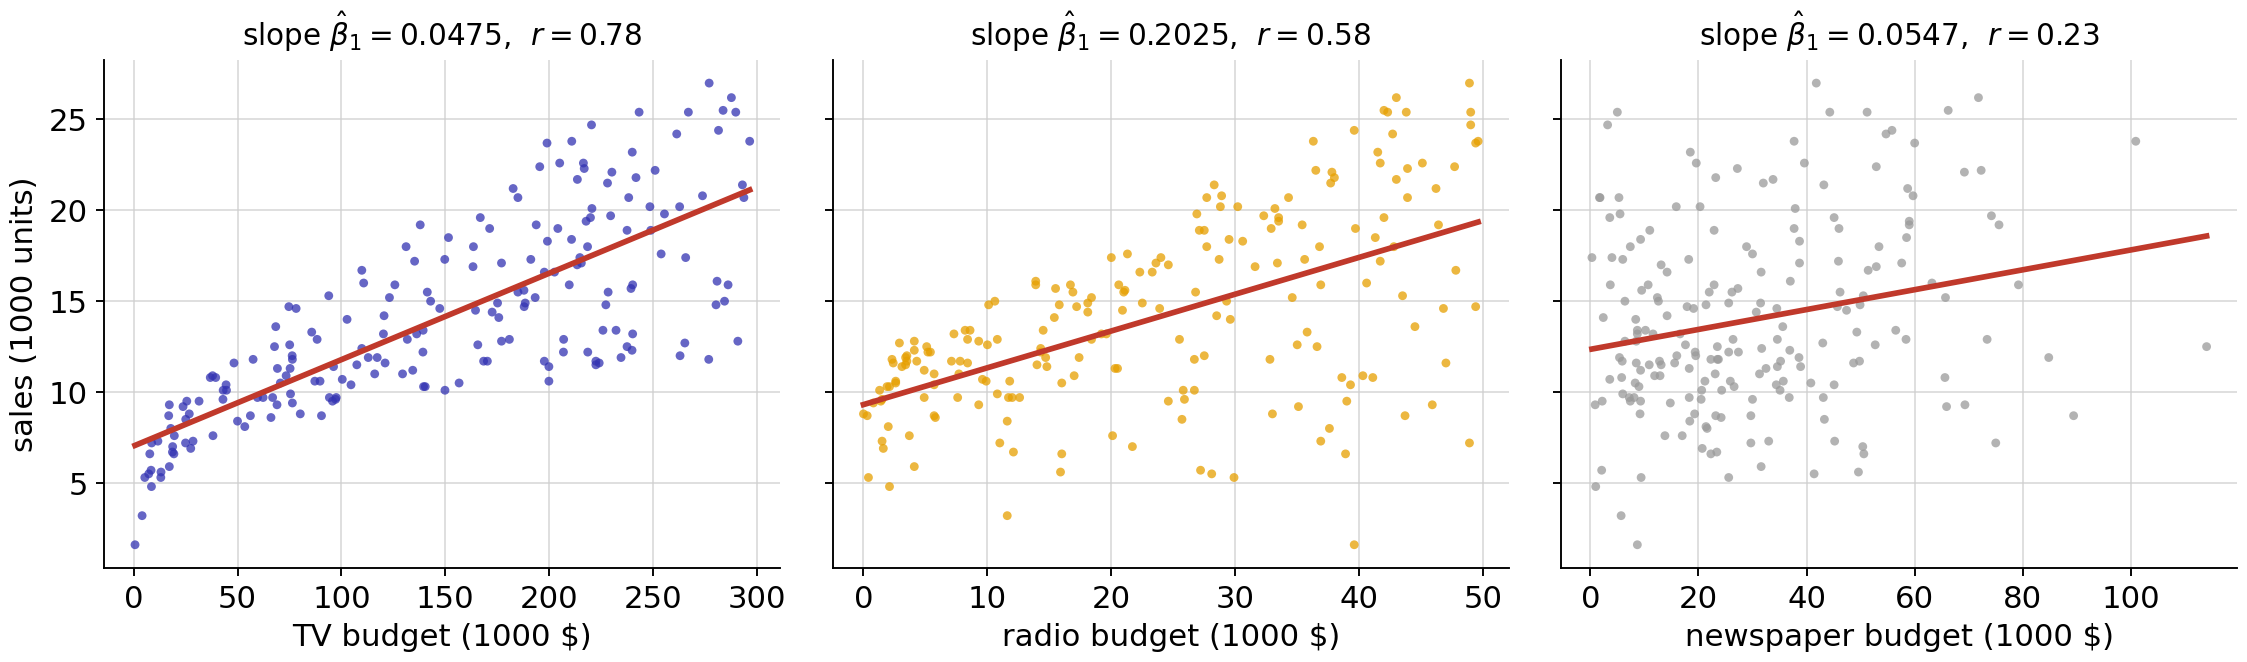
\includegraphics[width=0.92\textwidth,height=0.36\textheight,keepaspectratio]{images/reg_ad_three_predictors.png}
  \end{center}
  \sourcenote{Advertising data from James, Witten, Hastie, Tibshirani: \emph{An Introduction to Statistical Learning}, www.statlearning.com}
\end{frame}

\begin{frame}{The multiple linear regression model}
  \begin{block}{Model with $p$ explanatory variables}
    \[
      y_i = \beta_0 + \beta_1 x_{i1} + \beta_2 x_{i2} + \cdots + \beta_p x_{ip}
            + u_i,\qquad i=1,\dots,n,
    \]
    with the same four assumptions on the error terms $u_i$ as before.
  \end{block}
  \begin{block}{Interpretation of a coefficient}
    $\beta_j$ is the expected change in $Y$ when $X_j$ increases by one
    unit \textbf{and all other explanatory variables are held fixed}.
  \end{block}
  \begin{exampleblock}{Advertising}
    \[
      \texttt{sales}_i=\beta_0+\beta_1\,\texttt{TV}_i+\beta_2\,\texttt{radio}_i
        +\beta_3\,\texttt{newspaper}_i+u_i
    \]
  \end{exampleblock}
\end{frame}

\begin{frame}{Geometry: from a line to a plane}
  \begin{columns}[c]
    \begin{column}{0.52\textwidth}
      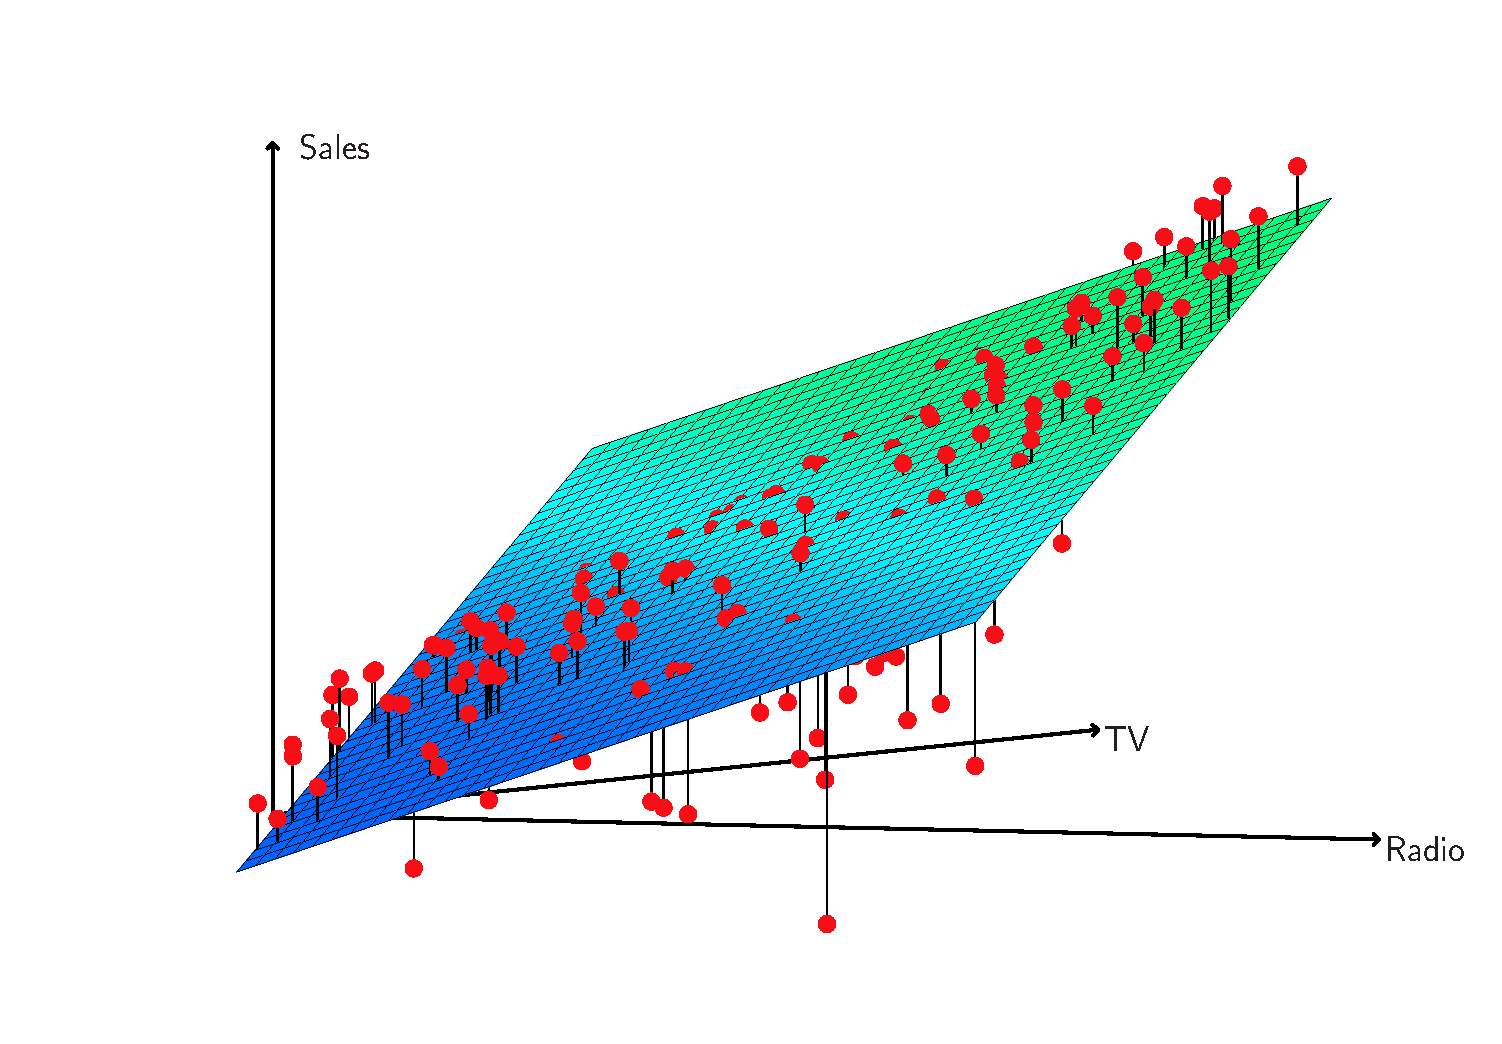
\includegraphics[width=\textwidth,height=0.72\textheight,keepaspectratio]{images/3_5.pdf}
    \end{column}
    \begin{column}{0.46\textwidth}
      \begin{itemize}\setlength{\itemsep}{4pt}
        \item With two explanatory variables the fitted model
              $\hat y=\hat\beta_0+\hat\beta_1x_1+\hat\beta_2x_2$ is a
              \textbf{plane}.
        \item The residuals are again the \emph{vertical} distances of
              the points from the plane.
        \item With $p$ variables: a ``hyperplane'' -- no longer drawable,
              but the same idea.
      \end{itemize}
    \end{column}
  \end{columns}
  \sourcenote{ISLR, Figure 3.5 (sales on TV and radio).}
\end{frame}

\begin{frame}{Least squares with several variables}
  \begin{block}{Same principle}
    Choose $\hat\beta_0,\hat\beta_1,\dots,\hat\beta_p$ such that the sum of
    squared residuals is minimal:
    \[
      \min_{\hat\beta_0,\dots,\hat\beta_p}\ \sum_{i=1}^n
      \bigl(y_i-\hat\beta_0-\hat\beta_1x_{i1}-\cdots-\hat\beta_px_{ip}\bigr)^2 .
    \]
  \end{block}
  \begin{itemize}\setlength{\itemsep}{3pt}
    \item The solution is unique as long as no variable is an exact
          linear combination of the others.
    \item There is no simple ``covariance over variance'' formula any more
          -- in matrix notation $\hat{\boldsymbol\beta}=(\mathbf X^\top\mathbf X)^{-1}\mathbf X^\top\mathbf y$,
          which software computes for us.
    \item Residuals, RSS, TSS and $R^2=1-\text{RSS}/\text{TSS}$ are defined
          exactly as before.
  \end{itemize}
\end{frame}

\begin{frame}[fragile]{Multiple regression with R}
  \begin{block}{Fitting the model}
\begin{lstlisting}
ad <- read.csv("../data/Advertising.csv", row.names = 1)
m3 <- lm(sales ~ TV + radio + newspaper, data = ad)  # sales explained by ...
summary(m3)
\end{lstlisting}
  \end{block}
\begin{lstlisting}[style=Rout]
Coefficients:
             Estimate Std. Error t value Pr(>|t|)
(Intercept)  2.938889   0.311908   9.422   <2e-16 ***
TV           0.045765   0.001395  32.809   <2e-16 ***
radio        0.188530   0.008611  21.893   <2e-16 ***
newspaper   -0.001037   0.005871  -0.177     0.86
---
Residual standard error: 1.686 on 196 degrees of freedom
Multiple R-squared:  0.8972,  Adjusted R-squared:  0.8956
F-statistic: 570.3 on 3 and 196 DF,  p-value: < 2.2e-16
\end{lstlisting}
\end{frame}

\subsection{Interpreting the coefficients}

\begin{frame}{Interpreting the coefficients -- ceteris paribus}
  \begin{exampleblock}{Advertising (budgets in $1000$\,\$, sales in $1000$ units)}
    \begin{itemize}\setlength{\itemsep}{4pt}
      \item \textbf{TV:} $\hat\beta_1=0.0458$ -- holding radio and newspaper
            fixed, $1000$\,\$ more TV budget goes along with about
            $0.0458\cdot1000=46$ additional units sold.
      \item \textbf{Radio:} $\hat\beta_2=0.1885$ -- holding TV and
            newspaper fixed, $1000$\,\$ more radio budget goes along with
            about $189$ additional units.
      \item \textbf{Newspaper:} $\hat\beta_3=-0.0010$ -- essentially zero
            once TV and radio are in the model.
      \item \textbf{Intercept:} $\hat\beta_0=2.94$ -- expected sales without
            any advertising ($2940$ units).
    \end{itemize}
  \end{exampleblock}
  \begin{alertblock}{The clause that matters}
    ``Holding the others fixed'' -- a coefficient in a multiple regression
    is a \emph{partial} effect, not the total association of $X_j$ with $Y$.
  \end{alertblock}
\end{frame}

\begin{frame}{Simple vs.\ multiple slopes}
  \begin{center}
    \renewcommand{\arraystretch}{1.3}
    \begin{tabular}{lrr}
      \toprule
      & \textbf{Simple regression} & \textbf{Multiple regression}\\
      & (one variable each) & (all three)\\
      \midrule
      TV         & $0.0475$ & $0.0458$ \\
      Radio      & $0.2025$ & $0.1885$ \\
      Newspaper  & $0.0547$\ \ ($p=0.001$) & $-0.0010$\ \ ($p=0.86$) \\
      \bottomrule
    \end{tabular}
  \end{center}
  \begin{alertblock}{What just happened?}
    On its own, newspaper looks like a significant driver of sales -- but its
    effect \emph{disappears} once TV and radio are in the model.
  \end{alertblock}
  \inworten{TV and radio hardly change -- they are almost uncorrelated with
  the other budgets. Newspaper changes completely.}
\end{frame}

\begin{frame}{Confounding: why the newspaper slope collapses}
  \begin{center}
    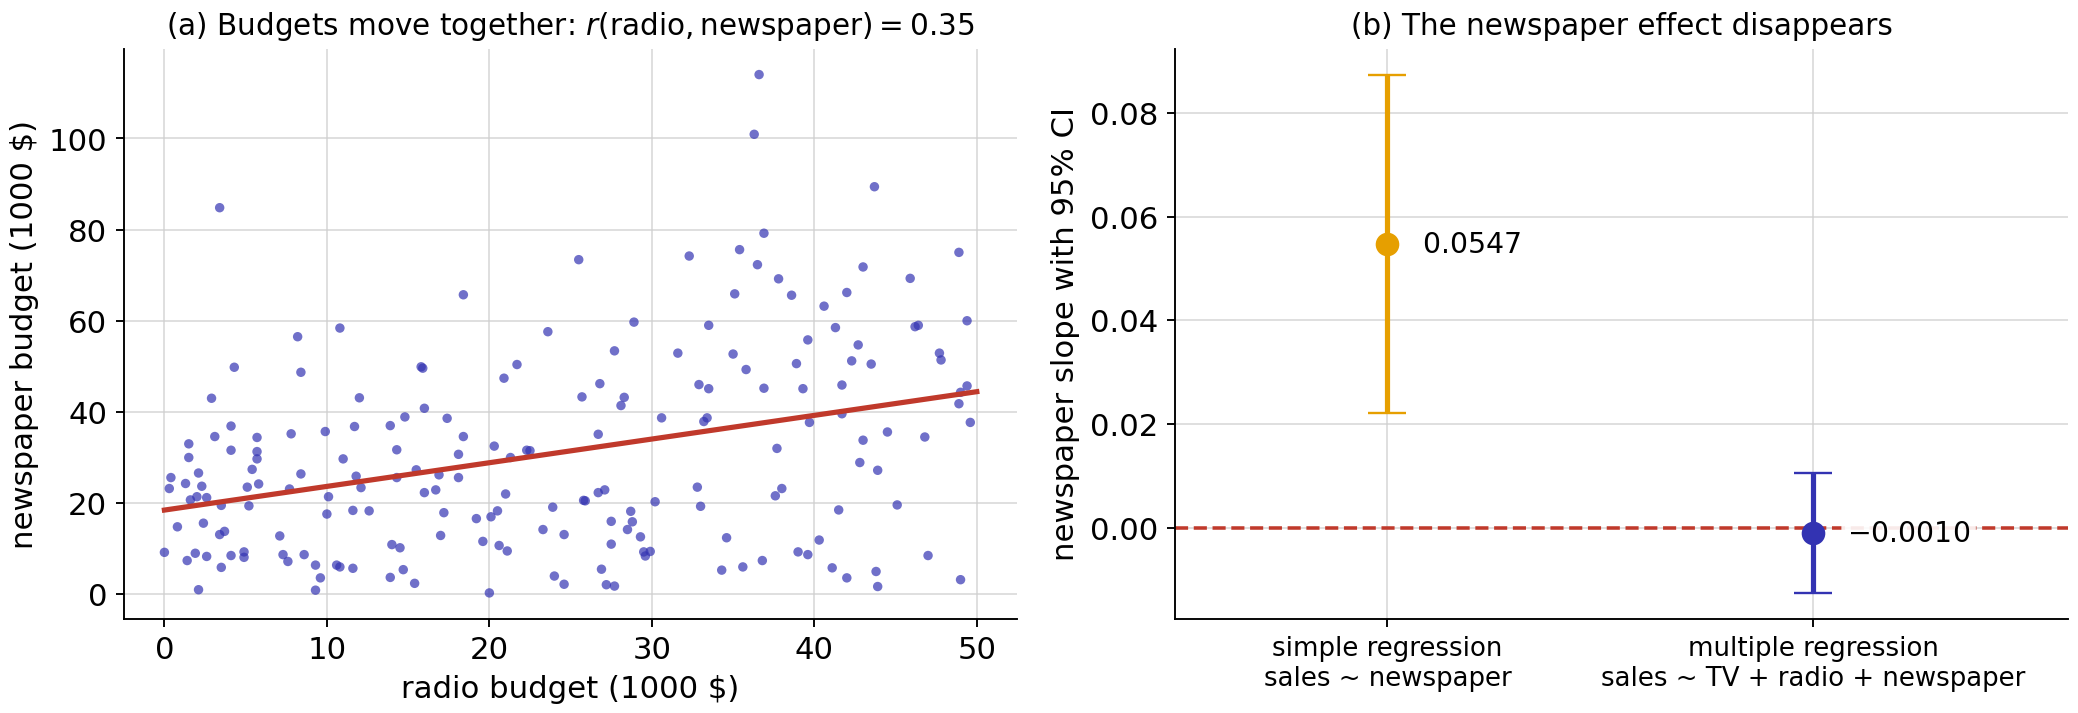
\includegraphics[width=0.92\textwidth,height=0.40\textheight,keepaspectratio]{images/reg_ad_confounding.png}
  \end{center}
  \begin{itemize}\setlength{\itemsep}{1pt}
    \item Markets with a large radio budget also spend more on newspapers
          ($r=0.35$) -- and radio really drives sales.
    \item In the simple regression, newspaper acts as a \textbf{proxy} for
          radio and ``borrows'' its effect.
  \end{itemize}
  \kernaussage{\textbf{Confounding:} a simple association can be produced
  by a third variable -- include all relevant variables.}
\end{frame}

\begin{frame}{Exercise -- why newspaper ``works'' alone}
  \begin{block}{Problem statement}
    A simple regression of sales on the newspaper budget gives a positive,
    significant slope ($0.0547$, $p=0.001$). In the multiple regression the
    newspaper coefficient is $-0.0010$ with $p=0.86$. The correlation between
    the newspaper and radio budgets is $0.35$.
    \begin{enumerate}
      \item Explain how newspaper can look useful on its own but useless in
            the joint model.
      \item Which variable is the actual driver?
      \item State the general lesson for interpreting simple correlations.
    \end{enumerate}
  \end{block}
\end{frame}

\begin{frame}{Solution -- why newspaper ``works'' alone}
  \begin{enumerate}\setlength{\itemsep}{4pt}
    \item \textbf{Confounding:} markets with high radio budgets also tend to
          have higher newspaper budgets. Radio raises sales. In the simple
          regression, the newspaper budget carries information about the
          radio budget that ``travels with it'' and inherits a positive
          slope. Once radio is included, radio absorbs this effect.
    \item \textbf{Driver:} radio (and TV). Newspaper is a stand-in for radio
          in the simple regression.
    \item \textbf{Lesson:} a simple association can be produced entirely by
          an omitted variable. To assess the effect of $X_j$
          \emph{holding the others fixed}, all relevant variables must be in
          the model.
  \end{enumerate}
  \begin{alertblock}{Common mistake}
    Concluding ``newspaper advertising can never work''. The model only says
    that newspaper adds nothing \emph{given TV and radio, in these data} --
    an observational, not a causal statement.
  \end{alertblock}
\end{frame}

\subsection{Inference for single coefficients}

\begin{frame}{$t$-test for a single coefficient}
  \begin{block}{Same recipe -- new degrees of freedom}
    \[
      H_0:\beta_j=0 \quad\text{vs.}\quad H_1:\beta_j\neq0,
      \qquad
      T=\frac{\hat\beta_j}{\mathrm{SE}(\hat\beta_j)}\;\sim\;t_{n-p-1}\ \text{under }H_0
    \]
  \end{block}
  \begin{itemize}\setlength{\itemsep}{3pt}
    \item $n-p-1$ degrees of freedom: $p+1$ coefficients were estimated
          (simple regression: $p=1$ $\Rightarrow$ $n-2$).
    \item $\hat\sigma=\sqrt{\text{RSS}/(n-p-1)}$; the standard errors are
          computed by software.
    \item \textbf{Reading of $H_0$:} ``$X_j$ adds nothing \emph{given the
          other variables in the model}''.
  \end{itemize}
  \begin{exampleblock}{Advertising ($n=200$, $p=3$, df $=196$, $t_{0.975;\,196}=1.972$)}
    Newspaper: $T=-0.0010/0.00587=-0.18$, $|T|<1.972$ $\Rightarrow$ keep
    $H_0$ ($p=0.86$). TV ($T=32.8$) and radio ($T=21.9$): reject.
  \end{exampleblock}
\end{frame}

\begin{frame}{Confidence intervals in multiple regression}
  \begin{block}{Construction}
    \[
      \text{CI}_{1-\alpha}(\beta_j)=\hat\beta_j\pm t_{1-\alpha/2,\,n-p-1}\cdot\mathrm{SE}(\hat\beta_j)
    \]
  \end{block}
  \begin{exampleblock}{Radio}
    \[
      0.18853\pm1.972\cdot0.00861=0.18853\pm0.01698=[\,0.1716\,;\,0.2055\,]
    \]
    Holding TV and newspaper fixed, $1000$\,\$ more radio budget goes along
    with $172$ to $206$ additional units sold.
  \end{exampleblock}
  \begin{center}
    \renewcommand{\arraystretch}{1.2}
    \begin{tabular}{lccc}
      \toprule
      & TV & radio & newspaper\\
      \midrule
      $95\,\%$ CI & $[0.0430;\,0.0485]$ & $[0.1715;\,0.2055]$ & $[-0.0126;\,0.0105]$\\
      \bottomrule
    \end{tabular}
  \end{center}
  \inworten{The newspaper interval contains $0$ -- the same message as its
  $t$-test.}
\end{frame}

\subsection{$F$-test}

\begin{frame}{Is \emph{any} explanatory variable useful? -- the $F$-test}
  \begin{block}{Hypotheses}
    \[
      H_0:\beta_1=\beta_2=\cdots=\beta_p=0
      \quad\text{vs.}\quad
      H_1:\text{at least one }\beta_j\neq0
    \]
  \end{block}
  \begin{block}{$F$-statistic}
    \[
      F=\frac{(\text{TSS}-\text{RSS})/p}{\text{RSS}/(n-p-1)}
      \;\sim\;F_{p,\,n-p-1}\ \text{under }H_0
    \]
  \end{block}
  \begin{itemize}
    \item Numerator: explained variation \emph{per explanatory variable}.
    \item Denominator: unexplained variation per residual degree of freedom
          ($=\hat\sigma^2$).
    \item Large $F$ $\Rightarrow$ the variables explain more than chance
          would $\Rightarrow$ reject $H_0$ (right-sided test).
  \end{itemize}
\end{frame}

\begin{frame}{$F$-test -- advertising example}
  \textbf{Given:} $\text{TSS}=5417.15$, $\text{RSS}=556.83$, $n=200$, $p=3$.
  \[
    F=\frac{(5417.15-556.83)/3}{556.83/196}=\frac{1620.11}{2.8410}=\mathbf{570.3}
    \;\gg\;2.65=F_{0.95;\,3,\,196}
  \]
  \begin{center}
    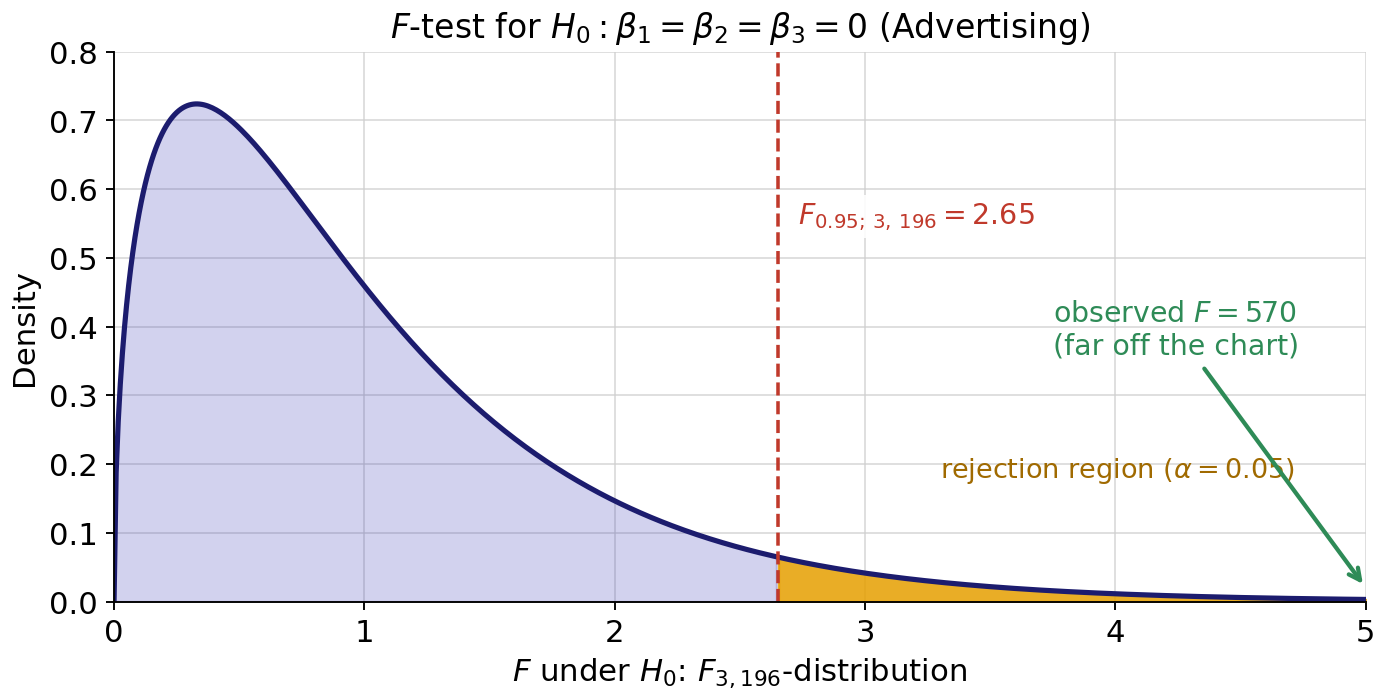
\includegraphics[width=0.72\textwidth,height=0.44\textheight,keepaspectratio]{images/reg_f_distribution.png}
  \end{center}
  \inworten{$H_0$ is rejected: at least one advertising medium is related to
  sales ($p<2.2\cdot10^{-16}$).}
\end{frame}

\begin{frame}{Why not just several $t$-tests?}
  \begin{alertblock}{Multiple testing}
    With $p$ explanatory variables and $\alpha=0.05$ per test, even if
    \emph{no} variable matters we expect about $0.05\cdot p$ ``significant''
    $t$-tests by chance alone -- with $p=20$ that is one false alarm per
    regression.
  \end{alertblock}
  \begin{block}{The $F$-test}
    One single test for all slopes together -- its Type~I error stays at
    $\alpha$, however many variables are in the model. Consult it
    \textbf{first}, then look at the individual $t$-tests.
  \end{block}
  \begin{exampleblock}{Special case}
    In simple regression ($p=1$) the $F$-test and the two-sided $t$-test
    are identical: $F=T^2$ (lamp: $125.2=(-11.19)^2$).
  \end{exampleblock}
\end{frame}

\begin{frame}{Exercise -- the $F$-test}
  \begin{block}{Problem statement}
    A multiple regression with $p=3$ explanatory variables is fitted on
    $n=100$ observations, giving $\text{TSS}=1000$ and $\text{RSS}=100$.
    \begin{enumerate}
      \item Compute $R^2$ and the $F$-statistic.
      \item Compare with $F_{0.95;\,3,\,96}=2.70$. What do you conclude?
      \item Suppose instead $100$ explanatory variables were all truly
            useless. About how many would appear ``significant'' at
            $\alpha=0.05$ in individual $t$-tests?
    \end{enumerate}
  \end{block}
\end{frame}

\begin{frame}{Solution -- the $F$-test}
  \begin{exampleblock}{(1) $R^2$ and $F$}
    \[
      R^2=1-\frac{100}{1000}=0.9,\qquad
      F=\frac{(1000-100)/3}{100/(100-3-1)}=\frac{300}{1.0417}=\mathbf{288}
    \]
  \end{exampleblock}
  \textbf{(2)} $288\gg2.70$ $\Rightarrow$ reject
  $H_0:\beta_1=\beta_2=\beta_3=0$: at least one variable is related to $Y$.

  \medskip
  \textbf{(3)} Each $t$-test rejects a true $H_0$ with probability
  $0.05$, so about $100\cdot0.05=5$ variables would look significant purely
  by chance -- which is why the $F$-test is consulted first.
  \begin{alertblock}{Common mistake}
    Reading a significant $F$ as ``all three variables matter''. It only
    says that \emph{at least one} does; the $t$-tests show which.
  \end{alertblock}
\end{frame}

\subsection{Goodness of fit and model choice}

\begin{frame}{$R^2$ and adjusted $R^2$}
  \begin{alertblock}{$R^2$ never decreases}
    Adding \emph{any} variable -- even pure noise -- can only lower RSS, so
    $R^2$ never decreases. Comparing models by $R^2$ always favours the
    larger model.
  \end{alertblock}
  \begin{block}{Adjusted $R^2$}
    \[
      \bar R^2=1-\frac{\text{RSS}/(n-p-1)}{\text{TSS}/(n-1)}
              =1-(1-R^2)\,\frac{n-1}{n-p-1}
    \]
    Penalises each additional variable: $\bar R^2$ only rises if the new
    variable reduces RSS by more than chance would.
  \end{block}
  \inworten{The residual standard error $\hat\sigma=\sqrt{\text{RSS}/(n-p-1)}$
  is penalised in the same way.}
\end{frame}

\begin{frame}{Model choice -- dropping newspaper}
  \begin{center}
    \renewcommand{\arraystretch}{1.3}
    \begin{tabular}{lccccc}
      \toprule
      Model & $\hat\beta_{\text{TV}}$ & $\hat\beta_{\text{radio}}$ & $R^2$ & $\bar R^2$ & $\hat\sigma$\\
      \midrule
      TV + radio + newspaper & $0.0458$ & $0.1885$ & $0.89721$ & $0.89564$ & $1.6855$\\
      TV + radio & $0.0458$ & $0.1880$ & $0.89719$ & $0.89615$ & $1.6814$\\
      \bottomrule
    \end{tabular}
  \end{center}
  \begin{exampleblock}{Decision}
    The slopes barely move, $R^2$ is practically unchanged, $\bar R^2$ rises
    and $\hat\sigma$ falls: \textbf{keep the simpler model}
    \texttt{sales \textasciitilde\ TV + radio}.
  \end{exampleblock}
  \begin{alertblock}{Common mistake}
    Arguing with the unchanged $R^2$ -- plain $R^2$ can only fall when a
    variable is dropped. Adjusted $R^2$ and $\hat\sigma$ are the fair judges.
  \end{alertblock}
\end{frame}

\begin{frame}{Prediction in multiple regression}
  \begin{block}{Same two intervals as before}
    For a market with TV $=100$ and radio $=20$ (in $1000$\,\$), the model
    \texttt{sales \textasciitilde\ TV + radio} predicts
    \[
      \hat y_0=2.921+0.04575\cdot100+0.18799\cdot20=11.26\ (1000\text{ units}).
    \]
  \end{block}
  \begin{center}
    \renewcommand{\arraystretch}{1.3}
    \begin{tabular}{lcl}
      \toprule
      & $95\,\%$ interval & Question\\
      \midrule
      Confidence interval & $[10.99;\,11.53]$ & mean sales of all such markets\\
      Prediction interval & $[\phantom{0}7.93;\,14.58]$ & sales of \emph{one} such market\\
      \bottomrule
    \end{tabular}
  \end{center}
  \kernaussage{With $n=200$ the mean is estimated precisely -- but a single
  market still varies by about $\pm2\hat\sigma\approx\pm3.3$.}
\end{frame}

\subsection{Qualitative explanatory variables}

\begin{frame}{What if an explanatory variable is categorical?}
  Many relevant variables are qualitative (student yes/no, region, brand)
  -- but regression needs numbers.
  \begin{block}{Solution: dummy variable ($0/1$ coding)}
    \[
      D_i=\begin{cases}1 & \text{if person $i$ is a student,}\\
                       0 & \text{otherwise (baseline).}\end{cases}
    \]
  \end{block}
  \begin{exampleblock}{Credit data ($n=400$): balance on student status}
    \[
      \widehat{\texttt{Balance}}=480.37+396.46\cdot D
    \]
    Non-students: $480.37$\,\$ on average; students:
    $480.37+396.46=876.83$\,\$. The coefficient of $D$ is the
    \textbf{difference in means} between the groups ($p<0.0001$).
  \end{exampleblock}
  \sourcenote{Credit data from James et al.: \emph{An Introduction to Statistical Learning}.}
\end{frame}

\begin{frame}{A dummy shifts the intercept}
  \begin{columns}[c]
    \begin{column}{0.6\textwidth}
      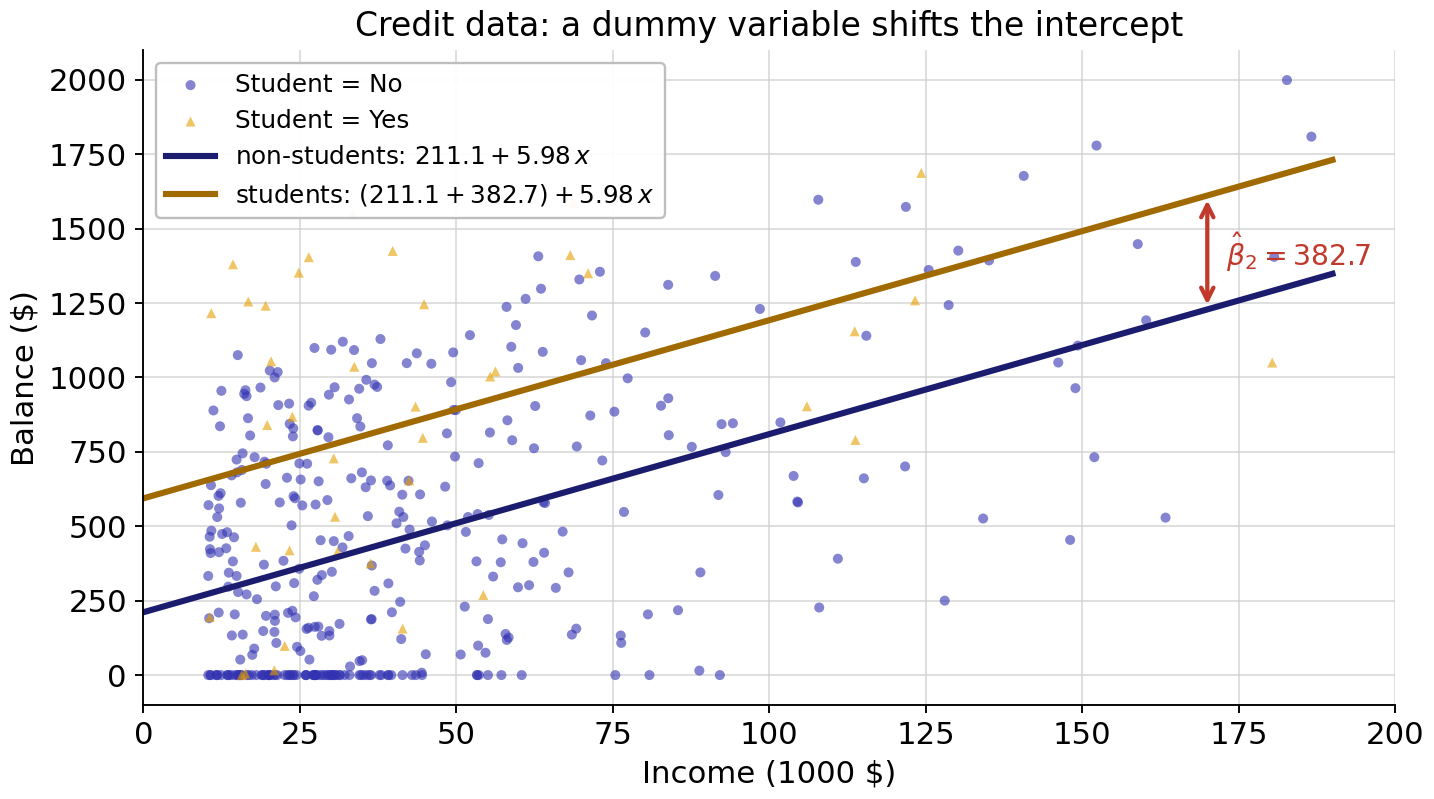
\includegraphics[width=\textwidth,height=0.72\textheight,keepaspectratio]{images/reg_credit_dummy.png}
    \end{column}
    \begin{column}{0.38\textwidth}
      \footnotesize
      \[
        \widehat{\texttt{Balance}}=211.1+5.98\,\texttt{Income}+382.7\,D
      \]
      \begin{itemize}\setlength{\itemsep}{3pt}
        \item Two \textbf{parallel} lines: same slope for income, intercept
              shifted by $\hat\beta_2=382.7$.
        \item Reading: at the \emph{same} income, students carry on average
              $382.7$\,\$ more balance.
      \end{itemize}
    \end{column}
  \end{columns}
\end{frame}

\begin{frame}{$K$ categories: use $K-1$ dummies}
  \begin{block}{Rule}
    A variable with $K$ categories is coded with $K-1$ dummies; the
    remaining category is the \textbf{baseline} represented by the intercept.
  \end{block}
  \begin{alertblock}{Why not $K$ dummies? (dummy variable trap)}
    The $K$ dummies always sum to $1$ -- exactly the column of the
    intercept. One variable would be an exact linear combination of the
    others, and least squares has no unique solution.
  \end{alertblock}
  \begin{exampleblock}{Credit data: region $\in\{$East, South, West$\}$, baseline East}
    \[
      \widehat{\texttt{Balance}}=531.00-12.50\,D_{\text{South}}-18.69\,D_{\text{West}}
    \]
    Both dummy coefficients are \emph{differences to East}
    ($p=0.83$ and $p=0.77$): no evidence for regional differences.
  \end{exampleblock}
\end{frame}

\begin{frame}{Exercise -- dummy coding}
  \begin{block}{Problem statement}
    \begin{enumerate}
      \item From $\widehat{\texttt{Balance}}=480.37+396.46\,D_{\text{Student}}$,
            give the predicted mean balance of students and of non-students.
            Interpret $396.46$.
      \item From $\widehat{\texttt{Balance}}=531.00-12.50\,D_{\text{South}}-18.69\,D_{\text{West}}$
            (baseline East), give the predicted mean balance in each region.
            How large is the difference between South and West?
      \item Why are only $K-1$ dummies used for a variable with $K$
            categories?
    \end{enumerate}
  \end{block}
\end{frame}

\begin{frame}{Solution -- dummy coding}
  \textbf{(1)} Non-students ($D=0$): $480.37$\,\$; students ($D=1$):
  $480.37+396.46=876.83$\,\$. The coefficient $396.46$ is the
  \textbf{difference in average balance} between students and non-students.

  \medskip
  \textbf{(2)} East $=531.00$, South $=531.00-12.50=518.50$, West
  $=531.00-18.69=512.31$. South vs.\ West: $-12.50-(-18.69)=+6.19$\,\$.

  \medskip
  \textbf{(3)} With $K$ dummies plus intercept, the dummies sum to the
  intercept column (dummy variable trap) -- the coefficients would not be
  identified. The dropped category becomes the baseline.
  \begin{alertblock}{Common mistake}
    Reading $-12.50$ as ``the mean of the South''. Dummy coefficients are
    \emph{contrasts} against the baseline, not group means.
  \end{alertblock}
\end{frame}

\subsection{Interactions}

\begin{frame}{When the effect of one variable depends on another}
  \begin{block}{Interaction model}
    \[
      y_i=\beta_0+\beta_1x_{i1}+\beta_2x_{i2}+\beta_3\,x_{i1}x_{i2}+u_i
    \]
    The effect of $x_1$ is now $\beta_1+\beta_3x_2$ -- it depends on $x_2$.
  \end{block}
  \begin{exampleblock}{Advertising: \texttt{sales \textasciitilde\ TV * radio}}
    \[
      \widehat{\texttt{sales}}=6.750+0.0191\,\texttt{TV}+0.0289\,\texttt{radio}
        +0.00109\,\texttt{TV}\cdot\texttt{radio}
    \]
    Interaction: $T=20.7$, $p<0.0001$; $R^2$ rises from $0.897$ to $0.968$.
  \end{exampleblock}
  \begin{alertblock}{Hierarchy principle}
    If $x_1x_2$ is in the model, keep $x_1$ and $x_2$ as well -- even if their
    own $t$-tests are not significant.
  \end{alertblock}
\end{frame}

\begin{frame}{Interaction, drawn: synergy between TV and radio}
  \begin{center}
    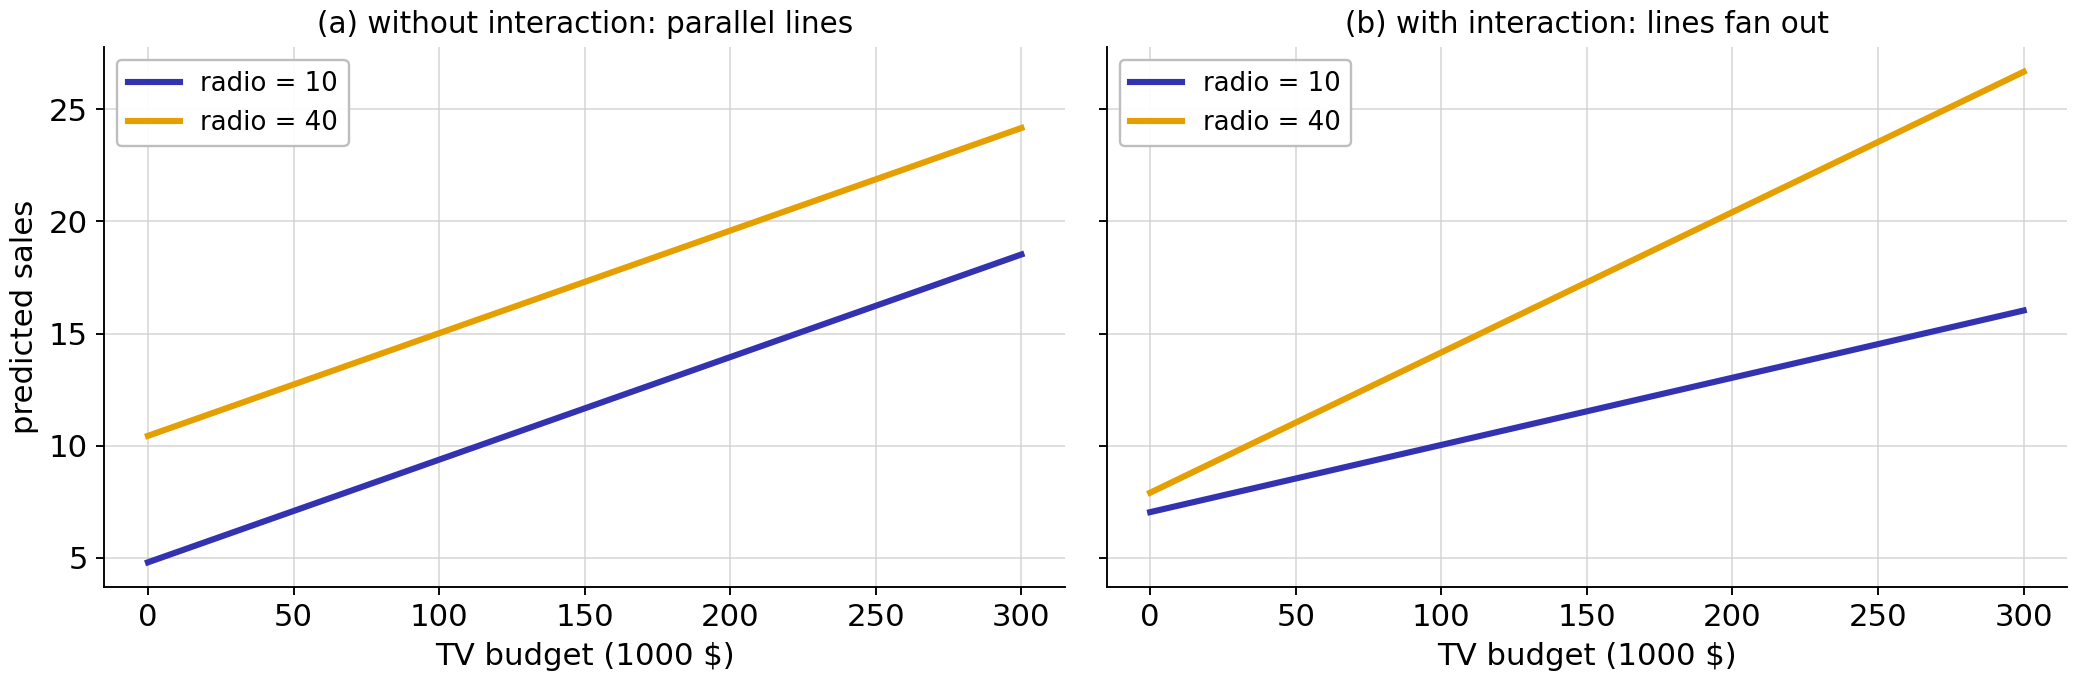
\includegraphics[width=0.95\textwidth,height=0.52\textheight,keepaspectratio]{images/reg_ad_interaction.png}
  \end{center}
  \begin{itemize}\setlength{\itemsep}{2pt}
    \item Effect of $1000$\,\$ more TV budget: $0.0191+0.00109\cdot\texttt{radio}$
          -- $0.030$ at radio $=10$, but $0.063$ at radio $=40$.
    \item Parallel lines $=$ no interaction; lines that fan out $=$ synergy.
  \end{itemize}
\end{frame}

% ============================================================================
% SECTION 7: DIAGNOSTICS
% ============================================================================
\section[Diagnostics]{Diagnostics in Multiple Regression}

\begin{frame}{The classical problems -- and how to spot them}
  \begin{center}
    \renewcommand{\arraystretch}{1.35}
    \begin{tabular}{@{}p{4.2cm}p{4.4cm}p{4.2cm}@{}}
      \toprule
      \textbf{Problem} & \textbf{Symptom} & \textbf{Tool}\\
      \midrule
      Non-linearity / missing term & curve in the residuals & residual plot\\
      Heteroscedasticity & funnel in the residuals & residual plot\\
      Non-normal errors & points off the line & QQ-plot\\
      Outliers, high leverage & single points dominate & $h_i$, residuals\\
      Collinearity & large SEs, unstable signs & correlations, VIF\\
      \bottomrule
    \end{tabular}
  \end{center}
  \kernaussage{The residual plot and the QQ-plot of the simple regression
  work unchanged in multiple regression -- plot the residuals against the
  fitted values $\hat y_i$.}
\end{frame}

\begin{frame}{Residual plot -- advertising}
  \begin{center}
    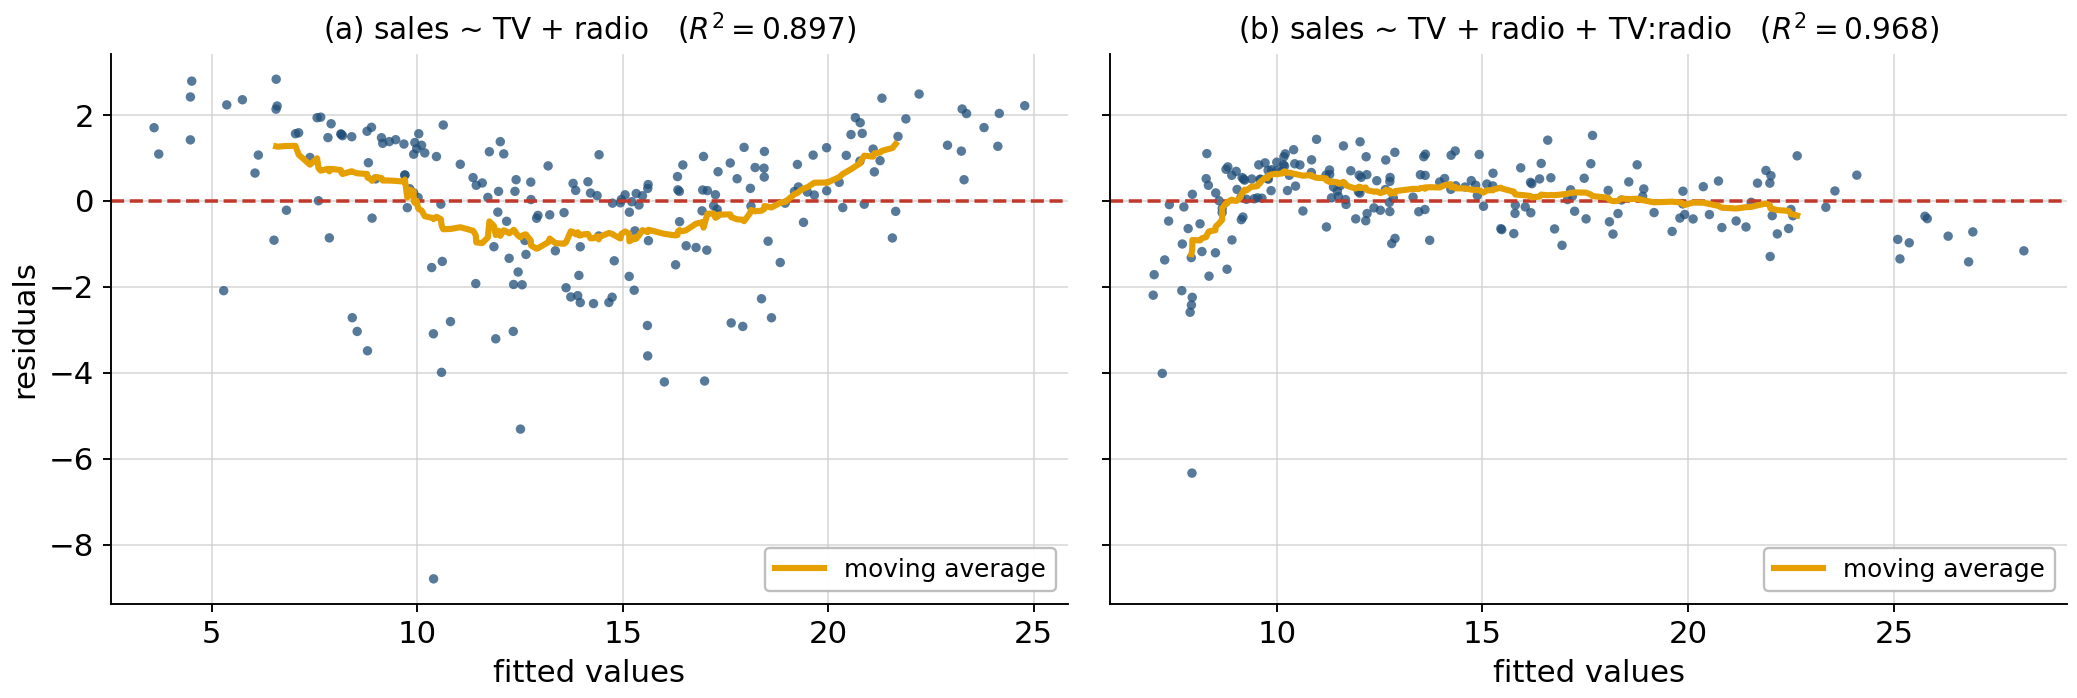
\includegraphics[width=0.95\textwidth,height=0.52\textheight,keepaspectratio]{images/reg_ad_residuals.png}
  \end{center}
  \begin{itemize}\setlength{\itemsep}{2pt}
    \item (a) The additive model leaves a \textbf{U-shaped} pattern: it
          over-predicts when one medium dominates and under-predicts when
          the budget is split.
    \item (b) With the interaction term the pattern largely disappears --
          the residuals \emph{told} us that a term was missing.
  \end{itemize}
\end{frame}

\begin{frame}{Outliers and leverage in multiple regression}
  \begin{columns}[T]
    \begin{column}{0.48\textwidth}
      \begin{block}{Outlier}
        A point with an unusually large residual $|\hat u_i|$ -- unusual
        in $y$.
      \end{block}
    \end{column}
    \begin{column}{0.48\textwidth}
      \begin{block}{High-leverage point}
        A point with unusual values of the explanatory variables -- unusual
        in $x$.
      \end{block}
    \end{column}
  \end{columns}
  \begin{block}{Rule of thumb for the leverage}
    The leverages $h_i$ average $(p+1)/n$; flag points with
    \[
      h_i>\frac{2(p+1)}{n}\qquad(\text{simple regression: }4/n).
    \]
  \end{block}
  \begin{alertblock}{Worst case}
    A point that is \emph{both} unusual in $x$ and badly fitted in $y$ can
    dominate the fit -- inspect it, compare the fit with and without it.
  \end{alertblock}
\end{frame}

\begin{frame}{Collinearity}
  \begin{block}{Definition}
    Two or more explanatory variables are (almost) linearly dependent --
    they carry nearly the same information.
  \end{block}
  \begin{center}
    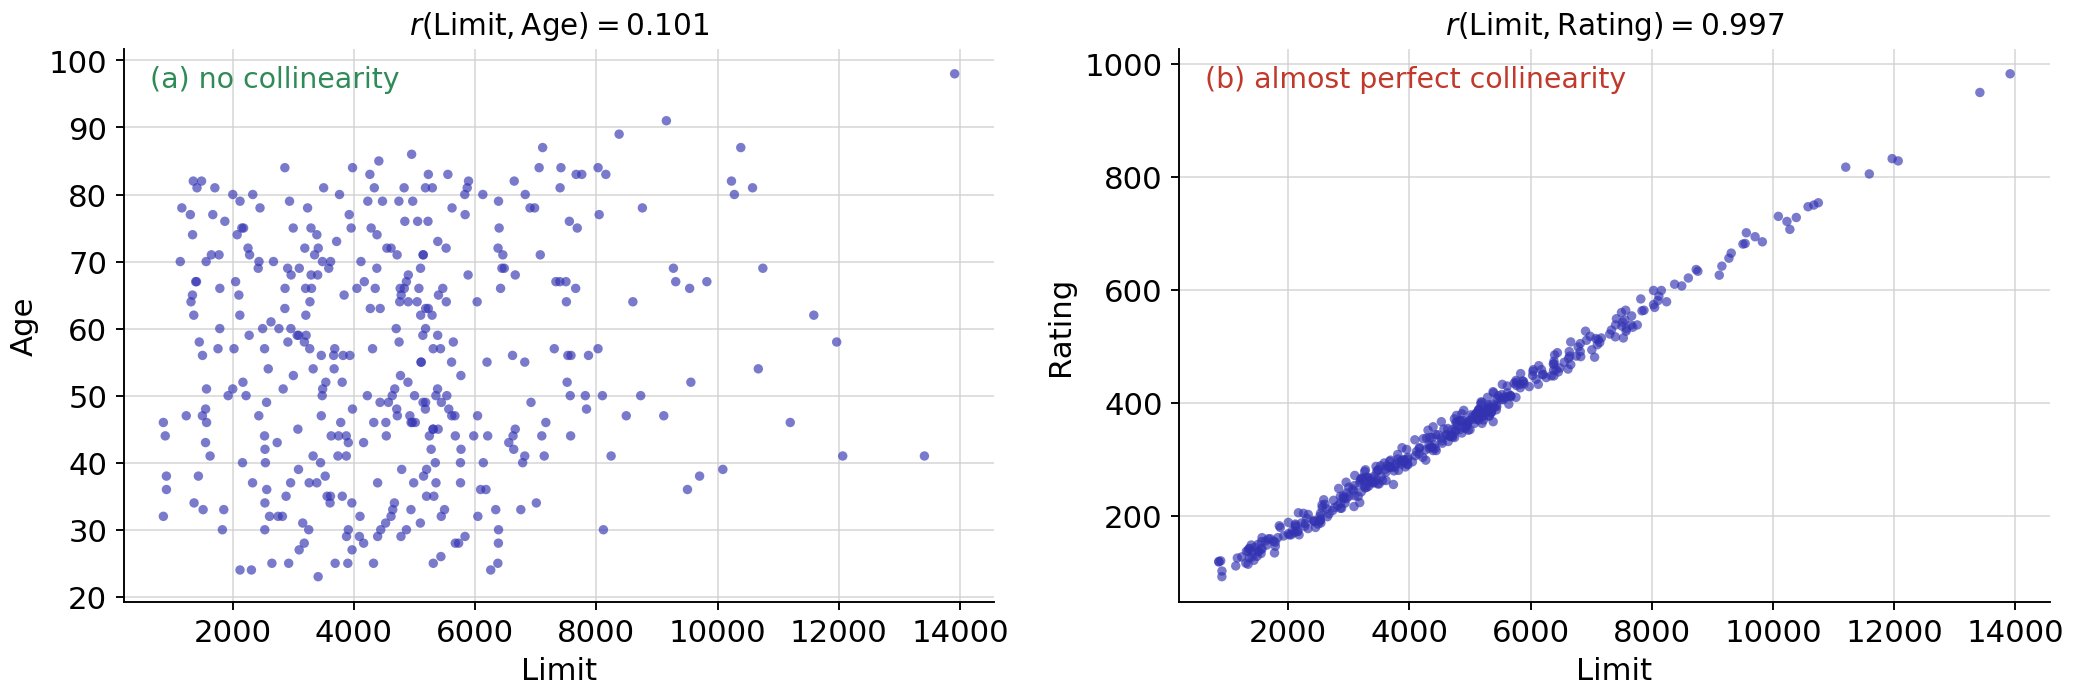
\includegraphics[width=0.9\textwidth,height=0.45\textheight,keepaspectratio]{images/reg_credit_collinearity.png}
  \end{center}
  \inworten{When two variables move in lockstep (right), the data cannot
  separate their individual effects -- holding one fixed while the other
  changes almost never happens.}
\end{frame}

\begin{frame}{Collinearity -- consequences in the credit data}
  \begin{center}
    \renewcommand{\arraystretch}{1.3}
    \begin{tabular}{lcccc}
      \toprule
      Model for \texttt{Balance} & $\hat\beta_{\text{Limit}}$ & $\mathrm{SE}(\hat\beta_{\text{Limit}})$ & $T$ & $p$\\
      \midrule
      \texttt{Age + Limit} & $0.1734$ & $0.0050$ & $34.5$ & $<0.0001$\\
      \texttt{Age + Limit + Rating} & $0.0190$ & $0.0630$ & $0.30$ & $0.76$\\
      \bottomrule
    \end{tabular}
  \end{center}
  \begin{alertblock}{Symptoms}
    Adding \texttt{Rating} (correlation $0.997$ with \texttt{Limit})
    multiplies the standard error of \texttt{Limit} by about $12.6$ -- the
    clearly relevant variable suddenly looks ``insignificant''.
  \end{alertblock}
  \inworten{Collinearity does not spoil the \emph{predictions} of the model;
  it spoils the \emph{attribution} of the effect to individual variables.}
\end{frame}

\begin{frame}{Variance inflation factor (VIF)}
  \begin{block}{Definition}
    \[
      \mathrm{VIF}_j=\frac{1}{1-R_j^2},
    \]
    where $R_j^2$ is the $R^2$ of a regression of $x_j$ on all
    \emph{other} explanatory variables.
  \end{block}
  \begin{itemize}\setlength{\itemsep}{3pt}
    \item $\mathrm{VIF}_j=1$: no collinearity; $\mathrm{VIF}_j>5$ (some
          authors: $10$): problematic.
    \item $\sqrt{\mathrm{VIF}_j}$ is the factor by which collinearity
          inflates $\mathrm{SE}(\hat\beta_j)$.
    \item Remedies: drop one of the redundant variables or combine them into
          one index.
  \end{itemize}
  \begin{exampleblock}{Credit data (\texttt{Age}, \texttt{Limit}, \texttt{Rating})}
    $\mathrm{VIF}_{\text{Age}}=1.01$, \quad
    $\mathrm{VIF}_{\text{Limit}}=160.6$, \quad
    $\mathrm{VIF}_{\text{Rating}}=160.7$ \quad
    ($\sqrt{160.6}=12.7$ -- matching the SE ratio $0.0630/0.0050$).
  \end{exampleblock}
\end{frame}

\begin{frame}{Exercise -- a diagnostics case study}
  \begin{block}{Problem statement}
    House prices are regressed on \texttt{size}, \texttt{bedrooms},
    \texttt{age} and \texttt{income} of the area ($n=400$, $p=4$). The
    diagnostics show:
    \begin{itemize}
      \item \textbf{Residual plot:} a clear U-shaped curve, and the spread
            of the residuals widens from left to right.
      \item \textbf{Leverage:} one point has $h_i=0.30$.
      \item \textbf{VIF:} size $8.9$, bedrooms $7.5$, age $1.3$, income $9.2$.
    \end{itemize}
    Name every problem and suggest a remedy for each.
  \end{block}
\end{frame}

\begin{frame}{Solution -- a diagnostics case study}
  \begin{enumerate}\setlength{\itemsep}{4pt}
    \item \textbf{U-shape -- non-linearity:} the linear model misses
          curvature. \emph{Remedy:} add e.g.\ $\texttt{size}^2$ or transform
          a variable ($\log\texttt{size}$).
    \item \textbf{Widening spread -- heteroscedasticity:} standard errors,
          $t$- and $F$-tests are unreliable. \emph{Remedy:} transform the
          response, e.g.\ $\log(\texttt{price})$.
    \item \textbf{Leverage:} threshold $2(p+1)/n=10/400=0.025$; $h_i=0.30$ is
          twelve times as large. \emph{Remedy:} inspect the point, compare the
          fit with and without it.
    \item \textbf{Collinearity:} VIFs of $7.5$--$9.2$ for size, bedrooms and
          income. \emph{Remedy:} drop or combine redundant variables (e.g.\
          keep size, drop bedrooms) and recompute the VIFs.
  \end{enumerate}
  \begin{alertblock}{Common mistake}
    Deleting flagged points automatically. Diagnostics call for
    \emph{inspection} and sensitivity checks -- not for blind removal.
  \end{alertblock}
\end{frame}

\begin{frame}[fragile]{Multiple regression with R -- overview}
  \begin{block}{Fitting, testing, comparing}
\begin{lstlisting}
m3 <- lm(sales ~ TV + radio + newspaper, data = ad)
summary(m3)            # t-tests, R^2, adjusted R^2, F-test
confint(m3)            # confidence intervals
m2 <- lm(sales ~ TV + radio, data = ad)
anova(m2, m3)          # F-test: does newspaper add anything? (p = 0.86)
\end{lstlisting}
  \end{block}
  \begin{block}{Dummies, interactions, diagnostics}
\begin{lstlisting}
lm(Balance ~ Income + Student, data = cr)   # factor -> dummy automatically
lm(sales ~ TV * radio, data = ad)           # TV + radio + TV:radio
plot(fitted(m2), resid(m2)); abline(h = 0)  # residual plot
hatvalues(m2)                               # leverages h_i
1 / (1 - summary(lm(Limit ~ Age + Rating, data = cr))$r.squared)  # VIF
\end{lstlisting}
  \end{block}
\end{frame}

% ============================================================================
% SECTION 8: SUMMARY
% ============================================================================
\section{Summary}

\begin{frame}{Summary 1 -- correlation and simple regression}
  \begin{center}
    \renewcommand{\arraystretch}{1.4}
    \begin{tabular}{l|l}
      \toprule
      \textbf{Quantity} & \textbf{Formula} \\
      \midrule
      Covariance & $s_{xy} = \frac{1}{n-1}\sum_{i=1}^{n}(x_i - \bar{x})(y_i - \bar{y})$ \\
      Correlation coefficient & $r_{xy} = \frac{s_{xy}}{s_x \, s_y}, \qquad -1 \leq r_{xy} \leq 1$ \\
      Model & $y_i = \beta_0 + \beta_1 x_i + u_i, \qquad \hat{y}_i = \hat{\beta}_0 + \hat{\beta}_1 x_i$\\
      Slope & $\hat{\beta}_1 = \frac{s_{xy}}{s_x^2}=\frac{S_{xy}}{S_{xx}}=r_{xy}\frac{s_y}{s_x}$ \\
      Intercept & $\hat{\beta}_0 = \bar{y} - \hat{\beta}_1 \bar{x}$ \\
      Coefficient of determination & $R^2 = \frac{\text{ESS}}{\text{TSS}} = 1 - \frac{\text{RSS}}{\text{TSS}} \;\bigl(= r_{xy}^2\text{ in simple regression}\bigr)$ \\
      \bottomrule
    \end{tabular}
  \end{center}
\end{frame}

\begin{frame}{Summary 2 -- model diagnostics}
  \begin{block}{Residuals $\hat{u}_i = y_i - \hat{y}_i$}
    \begin{itemize}
      \item \textbf{Residual plot} ($\hat y_i$ vs.\ $\hat u_i$): no pattern
            $\to$ model appropriate; curve $\to$ missing term; funnel $\to$
            heteroscedasticity.
      \item \textbf{QQ-plot}: points on the line $\to$ normality plausible.
    \end{itemize}
  \end{block}
  \begin{block}{Influential points and collinearity}
    \begin{itemize}
      \item Leverage $h_i>2(p+1)/n$ (simple regression $4/n$): inspect, do
            not delete blindly.
      \item $\mathrm{VIF}_j=1/(1-R_j^2)>5$: collinearity inflates
            $\mathrm{SE}(\hat\beta_j)$.
    \end{itemize}
  \end{block}
  \begin{exampleblock}{Coefficient of determination -- assessment}
    $R^2<0.6$: weak \quad $0.6\le R^2<0.8$: moderate \quad $R^2\ge0.8$:
    good \quad (context-dependent!)
  \end{exampleblock}
\end{frame}

\begin{frame}{Summary 3 -- inference for regression coefficients}
  \begin{block}{Standard error and residual standard error}
    \[
      \hat\sigma=\sqrt{\frac{\text{RSS}}{n-p-1}},\qquad
      \mathrm{SE}(\hat\beta_1)=\frac{\hat\sigma}{\sqrt{S_{xx}}}\ \ (\text{simple regression, }p=1)
    \]
  \end{block}
  \begin{block}{$t$-test, confidence interval, $p$-value}
    \[
      T=\frac{\hat\beta_j-\beta_{j,0}}{\mathrm{SE}(\hat\beta_j)}\sim t_{n-p-1},\qquad
      \hat\beta_j\pm t_{1-\alpha/2,\,n-p-1}\,\mathrm{SE}(\hat\beta_j),\qquad
      p=2\,F_{t,n-p-1}(-|T|)
    \]
  \end{block}
  \begin{block}{Prediction at $x_0$ (simple regression)}
    \[
      \hat y_0\pm t_{1-\alpha/2,\,n-2}\,\hat\sigma
      \sqrt{\underbrace{1}_{\text{PI only}}+\frac1n+\frac{(x_0-\bar x)^2}{S_{xx}}}
    \]
  \end{block}
\end{frame}

\begin{frame}{Summary 4 -- multiple regression}
  \begin{itemize}\setlength{\itemsep}{4pt}
    \item $\beta_j$: expected change in $Y$ per unit of $X_j$,
          \textbf{holding all other variables fixed}.
    \item \textbf{Confounding}: simple and multiple slopes can differ
          completely (newspaper: $0.055\to-0.001$).
    \item \textbf{$F$-test} for $H_0:\beta_1=\dots=\beta_p=0$:
          $F=\dfrac{(\text{TSS}-\text{RSS})/p}{\text{RSS}/(n-p-1)}$ -- first
          check, then the $t$-tests.
    \item \textbf{Adjusted} $\bar R^2=1-\dfrac{\text{RSS}/(n-p-1)}{\text{TSS}/(n-1)}$
          for comparing models of different size.
    \item \textbf{Dummies}: $K$ categories $\to$ $K-1$ dummies; coefficients
          are differences to the baseline.
    \item \textbf{Interactions} $x_1x_2$: the effect of $x_1$ depends on
          $x_2$; keep the main effects (hierarchy principle).
  \end{itemize}
\end{frame}

\begin{frame}[fragile]{Summary 5 -- important R commands}
  \begin{columns}[T]
    \begin{column}{0.5\textwidth}
      \begin{block}{Description and estimation}
\begin{lstlisting}
plot(x, y)              # scatter plot
cov(x, y); cor(x, y)    # covariance, corr.
reg <- lm(y ~ x)        # linear model
coef(reg)               # coefficients
abline(reg)             # regression line
summary(reg)            # SE, t, p, R^2, F
\end{lstlisting}
      \end{block}
    \end{column}
    \begin{column}{0.48\textwidth}
      \begin{block}{Inference and diagnostics}
\begin{lstlisting}
confint(reg)            # CIs
predict(reg, new, interval = "prediction")
plot(fitted(reg), resid(reg))
qqnorm(resid(reg)); qqline(resid(reg))
hatvalues(reg)          # leverages
lm(y ~ x1 + x2 + x3)    # multiple reg.
anova(small, large)     # F-test
\end{lstlisting}
      \end{block}
    \end{column}
  \end{columns}
\end{frame}

\begin{frame}{Five classic pitfalls -- final checklist}
  \small
  \begin{center}
    \renewcommand{\arraystretch}{1.45}
    \begin{tabular}{@{}>{\raggedright\arraybackslash}p{5.9cm}p{6.7cm}@{}}
      \toprule
      \textbf{Forbidden sentence \ \textcolor{hsbirot}{$\times$}} &
      \textbf{Correct version \ \textcolor{hsbigruen}{$\checkmark$}}\\
      \midrule
      ``$r_{xy}=0.97$, so price \emph{causes} the sales to fall.'' &
        Correlation and regression show association, not causation.\\
      ``$R^2$ is high, so the model is correct.'' &
        Check the residual plot; a curved relationship can have a high $R^2$.\\
      ``The slope is not significant, so $X$ has no effect.'' &
        No evidence found -- the CI shows which effects are still compatible.\\
      ``In the multiple regression, $\hat\beta_j$ is the total effect of $X_j$.'' &
        It is the effect \emph{holding the other variables fixed}.\\
      ``The model predicts $-1.17$ lamps at $125$ Euro.'' &
        No extrapolation far beyond the observed $x$-range.\\
      \bottomrule
    \end{tabular}
  \end{center}
\end{frame}

\begin{frame}{Outlook: Part 5 -- Classification}
  \begin{block}{What we have so far}
    Regression explains a \textbf{metric} variable $Y$ (sales, shoe size,
    balance) by one or several explanatory variables -- with full inference.
  \end{block}
  \begin{block}{Next part}
    What if $Y$ is \textbf{categorical} -- default yes/no, spam or not? A
    straight line would predict ``probabilities'' below $0$ or above $1$.
    \textbf{Logistic regression} keeps the linear model on the log-odds
    scale and reuses everything from this part: coefficients, standard
    errors, tests, confidence intervals and confounding.
  \end{block}
  \kernaussage{Classification = regression for categories -- plus the
  question of how to turn a probability into a decision.}
\end{frame}

\end{document}
